% Путівник гіпотезами проєкту «Моделювання потоку плазми в контурі токамаку»
% Компіляція: latexmk -xelatex main.tex
\documentclass[11pt,a4paper,oneside,notitlepage]{report}
% (преамбула винесена з main.tex; спільна для main і драйверів розділів)

% ---------- мова і шрифти ----------
\usepackage{fontspec}
\usepackage{polyglossia}
\setdefaultlanguage{ukrainian}
\setotherlanguage{english}
\gappto\captionsukrainian{\renewcommand{\bibname}{Бібліографія}\renewcommand{\refname}{Бібліографія}}
\setmainfont{cmunrm}[Extension=.otf,BoldFont=cmunbx,ItalicFont=cmunti,BoldItalicFont=cmunbi]
\setsansfont{cmunss}[Extension=.otf,BoldFont=cmunsx,ItalicFont=cmunsi,BoldItalicFont=cmunso]
\setmonofont{cmuntt}[Extension=.otf,BoldFont=cmuntb,ItalicFont=cmunit,BoldItalicFont=cmuntx]

% ---------- верстка ----------
\usepackage[a4paper,top=2cm,bottom=2.2cm,left=2.2cm,right=2cm]{geometry}
\usepackage{titlesec}
\titleformat{\chapter}[hang]{\Large\bfseries\sffamily}{\thechapter.}{0.6em}{}
\titlespacing*{\chapter}{0pt}{-10pt}{12pt}
\titleformat{\section}{\large\bfseries\sffamily}{\thesection}{0.6em}{}
\titleformat{\subsection}{\normalsize\bfseries\sffamily}{\thesubsection}{0.6em}{}
\usepackage{enumitem}
\usepackage{tocloft}
\usepackage{multicol}
\setlength{\cftbeforechapskip}{2pt}
\renewcommand{\cftsecfont}{\small}\renewcommand{\cftsecpagefont}{\small}
\setlength{\cftbeforetoctitleskip}{0pt}
\renewcommand{\cfttoctitlefont}{\large\bfseries\sffamily}
\setlength{\cftaftertoctitleskip}{4pt}
\setlength{\cftbeforesecskip}{0pt}

\setlist{itemsep=1pt,topsep=3pt,parsep=0pt}
\setlength{\emergencystretch}{3em}% довгі шляхи файлів у \texttt
\usepackage{booktabs,array,tabularx,longtable}
\renewcommand{\arraystretch}{1.12}
\usepackage{graphicx}
\graphicspath{{figures/}}
\usepackage[font=small,labelfont=bf,labelsep=period]{caption}
\usepackage{subcaption}
\usepackage[table]{xcolor}
\usepackage{tikz}
\usetikzlibrary{arrows.meta,calc,decorations.markings,positioning,shapes.geometric}

% ---------- математика і позначення ----------
\usepackage{notation}
\numberwithin{equation}{chapter}

% ---------- рамки ----------
\usepackage[most]{tcolorbox}
\tcbset{enhanced,breakable,boxrule=0.5pt,arc=1.5pt,left=5pt,right=5pt,top=3pt,bottom=3pt,
        fonttitle=\sffamily\bfseries\small\hypersetup{citecolor=white,linkcolor=white},before skip=6pt,after skip=6pt}
% стандартна теорія поза корпусом (рішення Q1)
\newtcolorbox{outofcorpus}[1][]{colback=gray!5,colframe=gray!60!black,
  title={Поза корпусом: стандартна теорія\ifx&#1&\else{} --- #1\fi}}
% приклад з корпусу: реальні установки й числа
\newtcolorbox{corpusexample}[1][]{colback=blue!3,colframe=blue!50!black,
  title={Приклад з корпусу\ifx&#1&\else{} --- #1\fi}}
% виведення з пропущеними рутинними кроками
\newtcolorbox{derivation}[1][]{colback=white,colframe=black!40,
  title={Виведення\ifx&#1&\else{} --- #1\fi}}
% практикум на коді проєкту
\newtcolorbox{practicum}[1][]{colback=green!4,colframe=green!40!black,
  title={Практикум\ifx&#1&\else{} --- #1\fi}}
% дослідницький трек: статуси з реєстрів Our try/00-decisions
\newtcolorbox{established}[1]{colback=teal!4,colframe=teal!60!black,
  title={Встановлено в проєкті [#1]}}
\newtcolorbox{conjecture}[1]{colback=orange!6,colframe=orange!70!black,
  title={Гіпотеза [#1] --- не перевірено}}
\newtcolorbox{refuted}[1]{colback=red!4,colframe=red!55!black,
  title={Спростовано [#1] --- повчальний приклад}}


% ---------- код (путівник) ----------
% minted (Pygments через latexminted); збірка: latexmk (див. latexmkrc: -shell-escape, PATH до Pygments).
% listings відмовились: під XeLaTeX він зсуває нумерацію, якщо над фрагментом є не-ASCII символи.
\usepackage{minted}
\usepackage{needspace}
\setminted{fontsize=\scriptsize,linenos,numbersep=6pt,breaklines,breakanywhere,frame=single,
  framesep=2mm,rulecolor=black!25,bgcolor=black!2,style=default}
% \code{шлях}{перший}{останній}{підпис} — фрагмент БЕЗПОСЕРЕДНЬО з файлу проєкту (через src/-посилання)
\newcommand{\code}[4]{\par\needspace{7\baselineskip}\noindent
  {\footnotesize\texttt{\detokenize{#1}}, рядки #2--#3\quad #4}\par\nopagebreak[4]\vspace{-2pt}
  \inputminted[firstline=#2,lastline=#3,firstnumber=#2]{python}{src/#1}}
% ---------- картки пунктів реєстру ----------
\newtcolorbox{itemcard}[2]{colback=black!2,colframe=black!55,title={#1\quad\normalfont\small #2}}

% ---------- посилання ----------
\usepackage[colorlinks=true,linkcolor=blue!50!black,citecolor=green!40!black,
            urlcolor=blue!60!black,bookmarksnumbered]{hyperref}
\usepackage{xurl}
\usepackage[ukrainian,nameinlink]{cleveref}

\title{\sffamily\bfseries Фізика плазми всередині токамака\\[4pt]
       \large Навчальний посібник (методичка)}
\author{На основі корпусу джерел проєкту «Моделювання потоку плазми в контурі токамаку»}
\date{2026}


\begin{document}
\thispagestyle{plain}
\begin{center}
{\LARGE\bfseries\sffamily Путівник гіпотезами проєкту}\\[3pt]
{\large\sffamily Що ми припускали, що перевірили, що спростували — і де це в коді}\\[2pt]
{\small Для студентів ФМФ КПІ \,·\, 2026}
\end{center}
\vspace{-1.5em}
{\footnotesize\renewcommand{\cftchapfont}{\bfseries\footnotesize}\renewcommand{\cftchappagefont}{\bfseries\footnotesize}
\renewcommand{\cftsecfont}{\footnotesize}\renewcommand{\cftsecpagefont}{\footnotesize}
\begin{multicols}{2}
\tableofcontents
\end{multicols}}
\chapter{Як читати путівник}\label{ch:g00}

Цей путівник --- не підручник і не звіт про успіх. Це історія проєкту, розказана через
його \emph{гіпотези}: що ми припускали, як перевіряли, що підтвердилося, що впало --- і що
виросло на місці спростованого. Фізику, на яку ми спираємося, викладено в методичці
\cite{Manual}; тут вона з'являється рівно настільки, наскільки потрібна, щоб зрозуміти
твердження й код, яким його перевіряли.

Кожен пункт розказано за однією схемою: (1)~що стверджується, простими словами і
формулою; (2)~звідки взялася ідея; (3)~що ми зробили (скрипт, параметри); (4)~що вийшло
(числа --- лише з \texttt{results.json}, реєстрів або повторного запуску); (5)~що з цього
випливло (статус і наступна ідея); (6)~де це в коді --- фрагмент, узятий \emph{безпосередньо}
з файлу проєкту, з поясненням по блоках; (7)~як відтворити й розвинути.

\section{Статуси і рамки}\label{sec:g00-status}

Усі статуси взято з реєстрів проєкту в тому вигляді, в якому їх узгоджено 2026-09-29
\cite{RegEst,RegConj,RegDec,RegQ,RegLog,RegViz}. Путівник статусів \emph{не присвоює}: якщо
реєстри між собою розходяться, ми про це кажемо, а не «виправляємо» мовчки.

\begin{center}\small
\begin{tabularx}{\textwidth}{@{}p{3.3cm}p{2.3cm}X@{}}
\toprule
Статус & Мітки & Що означає \\
\midrule
встановлено: виміряно & E (розд.~A), VE & виміряно \emph{власним кодом}; є скрипт і число \\
встановлено: прочитано & E (розд.~B) & прочитано у відкритому джерелі, з бібліографією \\
гіпотеза & C, VC & ще не перевірено; записано, \emph{що її спростує} і скільки коштує перевірка \\
спростовано & R, VR & власне твердження, яке перевірка збила; \emph{не видаляється} \\
відкрито & Q, VQ & питання, на яке ми не можемо відповісти самі (адресат указано) \\
відкладено & C9, C10 & гіпотеза, яку свідомо не перевіряємо (з причиною) \\
рішення & D & ухвалене рішення з \emph{умовою перегляду} \\
\bottomrule
\end{tabularx}
\end{center}

У тексті статуси позначено рамками:
\begin{established}{ID}
Рамка для встановленого (виміряного чи прочитаного). Число в ній --- з реєстру або з
повторного запуску.
\end{established}
\begin{conjecture}{ID}
Рамка для гіпотези. Завжди містить критерій спростування.
\end{conjecture}
\begin{refuted}{ID}
Рамка для спростованого. Показує, \emph{чим} спростовано і що з цього вийшло.
\end{refuted}
\noindent Для короткої довідки про пункт, який детально розібрано в іншому розділі,
вживаємо картку \texttt{itemcard} (ID і статус у заголовку).

\paragraph{Правила реєстрів.} Їх варто знати, бо вся структура путівника з них випливає
\cite{RegEst,RegConj}:
\begin{itemize}
\item \textbf{Правило входу} в реєстр встановленого: лише виміряне власним кодом або
  прочитане у відкритому джерелі --- «не здогадка, не правдоподібність, не „так роблять
  усі“».
\item \textbf{Правило входу} в реєстр гіпотез: усе неперевірене, з критерієм
  спростування і вартістю перевірки.
\item \textbf{Правило виходу:} перевірену гіпотезу переносять у встановлене --- або в
  розділ спростованого. \textbf{Нічого не зникає мовчки.} Кожна правка реєстрів має
  рядок у журналі змін \cite{RegLog} (дата, файл, «було~→~стало», причина, доказ).
\item \textbf{Правило цитування:} гіпотезу не можна вживати в концепті чи в матеріалах
  для учасників без позначки «гіпотеза».
\item Рішення (D) мають \emph{умову перегляду}; якщо вона настає, рішення переглядають,
  а не успадковують.
\end{itemize}
Станом на 2026-10-07 тринадцять власних тверджень перевірено й спростовано (R1--R13; R9~--- колишня C8,
зареєстрована 2026-09-29; R10 і R11~--- колишні C1 і C2, 2026-09-30; R12~--- половина C4 і
R13~--- колишня C5, обидві 2026-10-01) \cite{RegEst,RegConj}. Реєстр гіпотез наголошує: це не ознака
поганої роботи, а ознака того, що перевірка працює, а дві з них (R2, R7) після спростування дали
кращий результат, ніж містили до нього. Реєстр також стверджує, що спростоване не потрапляло в
концепт. Для R11 це не так: концепт подавав спектрально зважену втрату як «готове покращення»,
і це виправлено лише 2026-10-06 \cite{RegLog}. Знаменник «близько чотирнадцяти висунутих
гіпотез» у реєстрі з того часу не перераховувався.

\section{Простори імен}\label{sec:g00-ids}

Проєкт має кілька реєстрів із \emph{перетинними} мітками, тож завжди дивіться на префікс.
\begin{itemize}
\item \textbf{Батьківський реєстр} (\texttt{Our try/00-decisions/}): E1--E40 (виміряно:
  E1--E17, E30--E38, E40; прочитано: E18--E29, E39), R1--R13, C1--C10, Q1--Q13 (Q11, Q12 закриті),
  рішення D1--D9 \cite{RegEst,RegConj,RegQ,RegDec}.
\item \textbf{Глибокі розбори} --- теки \texttt{03-deep-dives/D1-\ldots, D2-\ldots, D3-\ldots}.
  Це \emph{не} рішення D1--D3! У путівнику пишемо «розбір~D1» проти «рішення~D1».
\item \textbf{Журнал верифікації}: V-A1--V-A4, V-D1--V-D4, V-B1--V-B5, V-C1--V-C4
  \cite{RegVerif}. До 2026-09-29 префікса \texttt{V-} не було, і «A2» чи «C3» зіткалися з
  іншими реєстрами; у старих текстах можна натрапити на старі мітки.
\item \textbf{Реєстр візуалізації} (\texttt{tokamak-3d-viz/\allowbreak findings.md}): VE1--VE33 (плюс
  VE11a), VR1--VR16, VC1--VC7, VQ1--VQ5 \cite{RegViz}. Тут «V» --- від
  \emph{visualization}: VC5 не має нічого спільного з C5.
\item \textbf{U1--U3} --- мітки путівника для трьох ненумерованих пунктів
  \texttt{tokamak-3d-viz/\allowbreak docs/\allowbreak COIL-BACKEND.md}: U1 (надлишок хаосу в
  бекенді котушок спричиняє гребінка бічних смуг --- спростовано), U2 (підлога хаосу в бекенді
  котушок: фізика чи числова похибка? --- відкрито), U3 (тримати векторний потенціал $\vect{A}$, а не поле $\Bvec$ на сітці;
  $\Bvec=\grad\times\vect{A}$ --- встановлено). Див.
  розділ~\ref{ch:g09}.
\item \textbf{N1--N7} --- знахідки координатора (\texttt{manual/\allowbreak tools/\allowbreak COORD\_NOTES.md}).
  Окремого реєстру вони не мають: 2026-09-29 їх зареєстровано в наявних \cite{RegLog}.
  N1 (ширина острова з $\psi$ як імпульсом, помилка в $\sqrt q$)~→ рецидив R4 і VR15 (а
  хибне пояснення, яке вона породила, --- VR16); N2 (функція Гріна отримувала $k$ замість
  $m=k^2$)~→ E33; N3 (C8 нездійсненна без джерела даних)~→ примітка до C8; N4 (поріг
  3\,\% у E10 пограничний)~→ уточнення E10, E11, E13; N5 (E14 без скрипта)~→ позначки в
  E14 і R6; N6 (GS-нев'язка ледь розрізняє моделі)~→ частковий результат C4; N7
  (GS-solver не запускався)~→ E34.
\item \textbf{H5} --- стара назва гіпотези «провал перенесення має топологічну складову»;
  окремого реєстру H-міток немає, H5 живе лише в R7 і в назві скрипта
  \texttt{04-novelty/\allowbreak h5\_transfer\_topology.py}.
\end{itemize}

\section{Як запускати код}\label{sec:g00-run}

Усі скрипти \texttt{Our try/}, код методички й більшість прикладів путівника
запускаються інтерпретатором із віртуального середовища стартового набору конкурсу
(Fusion Equilibrium Challenge \cite{FEC}); системний \texttt{python3} не має numpy.
У цьому середовищі є numpy~2.5, scipy~1.18, scikit-learn, matplotlib, pyarrow і
PyTorch~2.5 (перевірено 2026-09-29).
\begin{verbatim}
cd "fusion equilibrium challenge/starter"
.venv/bin/python "../../Our try/03-deep-dives/D1-psi-to-scalars/conditioning.py" \
    --frames 60 --seeds 3
\end{verbatim}
Де лежать дані:
\begin{itemize}
\item \texttt{fusion equilibrium challenge/starter/parquet\_data/} --- шість демо-розрядів
  (DIII-D 203702--203704, MAST 28348, 28350, 28351), формат Parquet, карти
  \texttt{efit\_psirz} $65\times65$;
\item \texttt{\ldots/starter/fusion\_scoring/} --- скорер (лише numpy) і маски
  (\texttt{masks/d3d\_envelope.npz}: сітка $R,Z$ і маска обвідної);
\item повний корпус (103,86~ГБ) --- на Hugging Face, \texttt{Sophelio/\allowbreak fusion-equilibrium-challenge},
  стрімінг без авторизації (розд.~\ref{ch:g01});
\item \texttt{tokamak-3d-viz} має власне середовище (див. README репозиторію: \texttt{python -m venv .venv}, потім \texttt{pip install -r requirements.txt}), дані й результати аналізу --- у
  \texttt{tokamak-3d-viz/data/};
\item \texttt{Tokamak-GS-solver} --- власне середовище (conda або pip, README; перевірено
  2026-09-29, Python~3.12).
\end{itemize}
Фрагменти коду в путівнику вставлено командою, що читає файл проєкту напряму через
посилання \texttt{guide/src/}: \texttt{ourtry/}~→ \texttt{Our try/}, \texttt{viz/}~→
\texttt{tokamak-3d-viz/}, \texttt{gs/}~→ \texttt{Tokamak-GS-solver/}, \texttt{fec/}~→
\texttt{fusion equilibrium challenge/}, \texttt{manualcode/}~→ \texttt{manual/code/}.
Номери рядків у лістингу --- справжні номери рядків файлу. Увага: деякі скрипти пишуть
результати у свою ж теку (наприклад, \texttt{branch\_mean.py} перезаписує
\texttt{results.json}); якщо хочете поекспериментувати, скопіюйте скрипт або скористайтеся
параметром \texttt{--out}, де він є.

\section{Карта: від спростування до нової ідеї}\label{sec:g00-map}

Рисунок~\ref{fig:g00-chains} показує головні ланцюжки путівника. Колір вузла --- статус
пункту \emph{зараз}; стрілка --- «з цього випливло». Більшість ланцюжків починається зі
спростування або з гіпотези, яку перевірка перетворила на щось інше. Праворуч --- розділ,
де ланцюжок розказано.

\begin{figure}[ht]
\centering
\begin{tikzpicture}[
  font=\sffamily\scriptsize,
  box/.style={draw,rounded corners=1.5pt,align=center,text width=2.12cm,
              minimum height=0.95cm,inner sep=2pt,line width=0.6pt},
  est/.style={box,fill=teal!10,draw=teal!60!black},
  con/.style={box,fill=orange!12,draw=orange!70!black},
  ref/.style={box,fill=red!8,draw=red!55!black},
  dec/.style={box,fill=blue!6,draw=blue!50!black},
  opn/.style={box,fill=gray!10,draw=gray!60!black},
  go/.style={-{Stealth[length=4pt]},line width=0.6pt},
  back/.style={go,dashed,red!55!black},
  node distance=0.34cm and 0.36cm,
  lab/.style={font=\sffamily\scriptsize\itshape,text=black!60}
]
% ряд 1: Бін
\node[ref] (r2) {\textbf{R2}\\Бін = плазма?};
\node[dec,right=of r2] (d8) {\textbf{D8}\\Бін як опуклий контроль};
\node[est,right=of d8] (e4) {\textbf{E4/E5}\\середнє гілок --- не розв'язок};
\node[con,right=of e4] (c7) {\textbf{C7}\\Deep Ritz: вибір гілки};
\draw[go] (r2)--(d8); \draw[go] (d8)--(e4); \draw[go] (e4)--(c7);
% ряд 2: перенесення
\node[con,below=of r2] (h5) {\textbf{H5}\\провал перенесення топологічний?};
\node[ref,right=of h5] (r7) {\textbf{R7}\\топологія вціліває};
\node[est,right=of r7] (e15) {\textbf{E15/E16}\\скелет 1O/0X на обох машинах};
\node[ref,right=of e15] (c8) {\textbf{C8$\to$R9}\\провали LCFS~--- артефакт знака};
\draw[go] (h5)--(r7); \draw[go] (r7)--(e15); \draw[go] (e15)--(c8);
% ряд 3: метрика
\node[est,below=of h5] (dd) {\textbf{розбори D1, D2}\\E1--E3; E4};
\node[est,right=of dd] (e6) {\textbf{E6--E8}\\GS-нев'язка лише з $\psi$};
\node[dec,right=of e6] (d6) {\textbf{D6}\\метрика $S'$};
\node[con,right=of d6] (c4) {\textbf{C4}\\GS-половина $\to$ R12};
\draw[go] (dd)--(e6); \draw[go] (e6)--(d6); \draw[go] (d6)--(c4);
% ряд 4: обернена задача
\node[ref,below=of dd] (c5) {\textbf{C5$\to$R13}\\Рівень~3 за 48~год? Фіт 0/40};
\node[est,right=of c5] (e30) {\textbf{E30--E32}\\пілот Tokamap};
\node[ref,right=of e30] (r8) {\textbf{R8}\\сума мод не симплектична};
\node[est,right=of r8] (ve21) {\textbf{VE21}\\$\Bvec=\grad\times(\psi\grad\tor)$};
\node[est,right=of ve21] (ve22) {\textbf{VE22--VE25}\\складність --- у фазах};
\node[est,right=of ve22] (ve30) {\textbf{VE30/VE31}\\слід; 2--6 мод};
\draw[go] (c5)--(e30); \draw[go] (e30)--(r8); \draw[go] (r8)--(ve21);
\draw[go] (ve21)--(ve22); \draw[go] (ve22)--(ve30);
% ряд 5: котушки
\node[con,below=of c5] (vc1) {\textbf{VC1}\\обвідна $\psiN^{m/2}$ = котушки?};
\node[ref,right=of vc1] (vr14) {\textbf{VR14}\\показник гуляє};
\node[est,right=of vr14] (u3) {\textbf{U3}\\тримати $\vect{A}$, а не $\Bvec$};
\draw[go] (vc1)--(vr14); \draw[go] (vr14)--(u3);
% ряд 6-7: острови і рецидив R4
\node[ref,below=of vc1] (vr12) {\textbf{VR12}\\дефіцит ширини --- засів?};
\node[est,right=of vr12] (ve18) {\textbf{VE18}\\маятникова формула (виправлена)};
\node[ref,right=of ve18] (vr15) {\textbf{VR15/VR16}\\помилка в $\sqrt q$};
\node[ref,below=of vr12] (r4) {\textbf{R4}\\$\psi$ як імпульс};
\node[est,right=of r4] (e19) {\textbf{E19}\\імпульс --- тороїдальний потік};
\draw[go] (vr12)--(ve18); \draw[go] (ve18)--(vr15);
\draw[go] (r4)--(e19);
\draw[back] (e19.east) -| node[pos=0.75,right,font=\sffamily\scriptsize,text=red!55!black]{рецидив у коді (N1)} (vr15.south);
% підписи розділів
\node[lab,anchor=west,xshift=1.5mm] at (c7.east) {розд.~\ref{ch:g03}};
\node[lab,anchor=west,xshift=1.5mm] at (c8.east) {розд.~\ref{ch:g06}};
\node[lab,anchor=west,xshift=1.5mm] at (c4.east) {розд.~\ref{ch:g02}, \ref{ch:g04}};
\node[lab,anchor=north,yshift=-0.5mm] at (ve30.south) {розд.~\ref{ch:g07}};
\node[lab,anchor=west,xshift=1.5mm] at (u3.east) {розд.~\ref{ch:g09}};
\node[lab,anchor=west,xshift=1.5mm] at (vr15.east) {розд.~\ref{ch:g08}};
% легенда
\node[est,text width=1.75cm,minimum height=0.5cm,below=0.55cm of r4] (l1) {встановлено};
\node[con,text width=1.75cm,minimum height=0.5cm,right=0.2cm of l1] (l2) {гіпотеза};
\node[ref,text width=1.75cm,minimum height=0.5cm,right=0.2cm of l2] (l3) {спростовано};
\node[dec,text width=1.75cm,minimum height=0.5cm,right=0.2cm of l3] (l4) {рішення};
\draw[back] ([xshift=3mm]l4.east) -- ++(8mm,0) node[right,text=black]{повернення старої помилки};
\end{tikzpicture}
\caption{Головні ланцюжки «спростування~/ гіпотеза~→ нова ідея». Колір --- поточний статус
за реєстрами на 2026-10-07 \cite{RegEst,RegConj,RegDec,RegViz}. VE18 після 2026-09-29
переформульовано: старе пояснення «дефіцит ширини = стохастичний шар» тепер VR16.
C5 закрито 2026-10-01: базовий нелінійний фіт не дійшов до рівня шуму (R13), бо ландшафт
нев'язки «скляний» (E40).}
\label{fig:g00-chains}
\end{figure}

Кілька ланцюжків варто прочитати вголос, бо вони задають тон решті путівника.
\begin{itemize}
\item \textbf{R2~→ D8~→ E4/E5~→ C7.} Гіпотеза «критичний стан Біна і вільна межа плазми ---
  одна математика» впала на опуклості. Врятована версія --- Бін як \emph{опуклий
  контроль} --- дала точний вимір: середнє двох гілок нелінійної задачі не є розв'язком
  (розд.~\ref{ch:g03}).
\item \textbf{H5~→ R7~→ E15/E16.} Ми чекали, що перенесення DIII-D~→ MAST ламає
  топологію $\psi$. Вийшло навпаки: значення ламаються, топологія --- ні. Інверсія виявилась
  кориснішою за гіпотезу (розд.~\ref{ch:g06}).
\item \textbf{C5~→ \ldots~→ VE30/VE31.} Пілот оберненої задачі наштовхнувся на власну
  помилку (R8: узагальнена мапа не зберігає потік); блокер зняв структурний прийом
  $\Bvec=\grad\times(\psi\grad\tor)$ (VE21), і тоді з'ясувалося, що в лінеаризованій постановці
  складність задачі задає вибір спостережуваного, а не фізика. Нелінійна перевірка закрила
  гіпотезу: інформація в даних є, але базовий фіт застрягає на «скляному» ландшафті (R13, E40;
  розд.~\ref{ch:g07}).
\item \textbf{R4~→ E19~→ VR15.} Помилку «$\psi$ як канонічний імпульс» спростували ще в
  рецензії літератури --- і вона однаково повернулася в коді візуалізації, завищивши ширину
  острова в $\sqrt q$ разів. Звідси правило «нічого не зникає мовчки»: спростоване
  лишається в реєстрі саме для того, щоб його впізнали при рецидиві (розд.~\ref{ch:g08}).
\end{itemize}

\chapter{Звідки все почалося: вибір задачі}\label{ch:g01}

Проєкт почався не з фізики, а з організаційного питання: \emph{яку задачу дати студентам
на хакатоні ФМФ}, щоб за 24--48 годин вони могли зробити щось справжнє, а журі --- чесно
це оцінити. Відповідь, до якої ми прийшли 2026-09-22, --- «реконструкція магнітного
потоку $\psi(R,Z)$ без магнітних датчиків, з метрикою, яка питає, чи це взагалі
рівновага». Цей розділ пояснює, чому саме так, які варіанти ми відкинули і які факти
(E25--E29) та відкриті питання (Q10--Q13) стоять за рішенням. Фізику рівноваги й
величини $\psi$, $\qnf$, $\betaN$, $\li$ див. у \cite{Manual}, розд.~3.

\section{Критерій вибору: де стеля, а де простір}\label{sec:g01-criterion}

Правило, яким ми відсіювали задачі, записано у файлі \texttt{saturated-vs-headroom.md} (тека
\texttt{Our try/01-landscape/}): \emph{задача придатна для хакатону, якщо найкращий
опублікований результат помітно нижчий за очевидну стелю}. Інакше студентська команда за
дві доби нічого не зрушить, а таблиця лідерів перетвориться на лотерею шуму.

\begin{established}{E25 (прочитано)}
Прогноз зриву (disruption) насичений \emph{і} має закриті дані: AUC~0,974 всередині машини;
DisruptionBench --- харнес без даних, архівований 2025-07-21 \cite{RegEst,Spangher2025}.
\end{established}
\noindent Число 0,974 (CCNN на Alcator C-Mod) у наших файлах позначено \texttt{[S]} --- взято зі
зведення пошуку, а не з відкритої статті; факт «архівовано без даних» --- \texttt{[V]}.
Залишковий розрив у прогнозі зриву --- операційний (частота хибних тривог за фіксованого часу
попередження), а не в AUC. Дані C-Mod, DIII-D, EAST не випущені, JET закрито юридично,
KSTAR публічного набору не має (\texttt{02-field-map/E-disruption-why-not.md}). Фізику
зривів див. \cite{Manual}, розд.~10.

Натомість простір знайшовся там, де наявні бенчмарки \emph{не міряють}: фізична
узгодженість (нев'язка рівняння Ґреда--Шафранова), калібрування невизначеності,
обумовленість відображення $\psi\mapsto$ скаляри (розд.~\ref{ch:g02}) і неєдиність
розв'язку (розд.~\ref{ch:g03}). Реконструкція $\psi$ всередині DIII-D \emph{за наявною
метрикою} теж близька до стелі: стартовий набір уже дає $S=0{,}8143$ на 20 відкладених
розрядах, а шлюз Challenge~2 поставлено на 0,85 (\texttt{saturated-vs-headroom.md}, \texttt{[V]}).
Тому ми змінюємо \emph{метрику}, а не задачу.

\section{Рішення D1--D9}\label{sec:g01-decisions}

Реєстр рішень \cite{RegDec} (версія~1, 2026-09-22) має незвичну колонку: «що б його
змінило». Рішення без умови перегляду мовчки успадковується, навіть коли обставини
змінилися.

\begin{center}\small
\begin{tabularx}{\textwidth}{@{}p{0.7cm}Xp{4.3cm}@{}}
\toprule
& Рішення & Що б його змінило \\
\midrule
D1 & ядро --- реконструкція $\psi(R,Z)$, а не прогноз зриву & відкритий датасет зривів із
  мітками $t_{\text{ТГ}}$ \\
D2 & конвеєр рівновага~→ стійкість~→ зрив --- лише в наративі; одна оцінювана задача +
  3--4 номінації на тому самому $\psi$ & горизонт 3+ місяці або 3+ інженери \\
D3 & два треки: базовий (starter kit + таблиця) і дослідницький (журі) & однорідна
  аудиторія \\
D4 & дані sim-to-real: навчання на синтетиці, тест на реальних розрядах & синтетика надто
  «легка» \\
D5 & синтетика з \texttt{FreeGS}/\texttt{FreeGSNKE}/\texttt{TokaLab}, свого генератора не
  пишемо & жоден не дає потрібної геометрії \\
D6 & метрика $S'$ = метрика Sophelio + GS-нев'язка + калібрування UQ & перевірка V-A4
  знайде, що хтось це вже робить \\
D7 & аналіз українською, підсумкові артефакти --- англійською & --- \\
D8 & \textbf{закрито 2026-09-22}: надпровідність не окрема тема; Бін --- опуклий контроль
  у розборі D2 & нічого: питання закрито доказово \\
D9 & розрахунок квенчу магніта --- не оцінювана задача & виміряні дані по котушках під час
  зривів \\
\bottomrule
\end{tabularx}
\end{center}

Два зауваження про історію цих рядків (журнал змін \cite{RegLog}, п.~23 і~26). До
2026-09-29 обґрунтування D1 посилалося на «див.~D9», хоча D9 --- про квенч магніта; тепер
там стоїть посилання на відкинутий варіант «хакатон із прогнозу зриву», E25 і
\texttt{E-disruption-why-not.md}. А англійський підсумок реєстру ще тиждень після
закриття D8 казав, що надпровідність «відкладено до огляду літератури». Обидві неточності
виправлено відкрито, зі старим текстом у журналі.

\paragraph{Відкинуті варіанти.} Реєстр зберігає шість варіантів, від яких ми відмовилися,
разом із причинами:
\begin{enumerate}
\item \emph{Хакатон із прогнозу зриву} (готовий внутрішній протокол) --- насичено, дані
  закриті, а симулятора \texttt{tok-sym-core}, на який спирався протокол, у проєкті немає.
\item \emph{Клон Fusion Equilibrium Challenge} --- змагання живе (Phase~1 до 2026-10-18,
  176~учасників, 684~подання), клонувати надлишково.
\item \emph{Участь у Sophelio командою факультету} --- відхилено: чужий дедлайн відволікає.
\item \emph{Генератор даних на \texttt{fusionsimulator.io}} --- коду локально немає,
  ліцензія суперечлива (Q10), 2,5--3 тижні роботи.
\item \emph{Надпровідність як оцінювана задача} --- немає ground truth; один член втрат
  домінує в $\approx490$ разів, тож «модель» зводиться до підстановки у формулу.
\item \emph{Гіпотеза «Бін~$\leftrightarrow$ вільна межа плазми --- одна математика»} ---
  спростовано власною перевіркою (R2); врятовано переформульовану версію D8
  (розд.~\ref{ch:g03}).
\end{enumerate}
Сюди ж реєстр відносить спростоване твердження «ніхто не нав'язує інтегральну крайову
умову жорстко» (R1, перевірка V-A2; спростовано роботою \cite{McClenaghan2024}). І три визнані ризики, на які план не розраховує:
горизонт менше місяця; формат 24--48~год погано сумісний із дослідницьким треком; команда
--- фактично одна людина плюс 2--4 помічники.

\section{Дані й ліцензії: E26--E29, Q10--Q13}\label{sec:g01-data}

Рішення D4 спирається на відкриті дані, тож першою роботою було \emph{переміряти} все, що
про ці дані пишуть офіційні джерела. Результат --- чотири прочитані факти і чотири зовнішні
питання.

\begin{established}{E26--E29 (прочитано/перевірено)}
\begin{itemize}
\item[E26] Корпус Sophelio --- \textbf{103,86~ГБ, 9\,121 розряд} (7\,041 \texttt{diii\_d\_train}
  + 874 \texttt{diii\_d\_public\_test} + 1\,206 \texttt{mast\_public\_test}), виміряно
  через HF API.
\item[E27] Член Consistency метрики усереднює \textbf{сім} скалярів, не вісім.
\item[E28] Ліцензії: HDB5 --- CC~BY~4.0; ConStellaration --- MIT; Sophelio --- CC~BY~4.0;
  FAIR-MAST --- CC~BY-SA~4.0 із поширенням на похідні бази через §4(b).
\item[E29] Код стартового набору справді MIT; статус \texttt{NOASSERTION} на GitHub
  спричинений дописаним розділом «NOTE ON SCOPE».
\end{itemize}
\end{established}

Чому це не дрібниці. Офіційні числа суперечать самі собі (V-B1, V-B2 \cite{RegVerif}):
на сайті 98~ГБ, у статті 133~ГБ; кількість розрядів в анотації статті й у її тексті
різна. Тому для статистики датасету статтю \cite{FEC} ми вважаємо ненадійною, а
перелічуємо файли самі. Так само з E27: єдине «вісім» --- у застарілій спливній підказці на
сайті, а код скорера (нижче) каже «сім»; для нас код надійніший за сайт.

\begin{center}\small
\begin{tabularx}{\textwidth}{@{}p{0.8cm}Xp{3.3cm}@{}}
\toprule
& Питання & Статус \\
\midrule
Q10 & умови поширення даних, згенерованих \texttt{fusionsimulator.io} (README водночас
  «MIT» і «All rights reserved») & відкрите; нічого похідного не публікуємо \\
Q11 & ліцензія ITPA HDB5 & закрите: CC~BY~4.0 (поле власників порожнє) \\
Q12 & атрибуція скорера й даних Sophelio & закрите: код MIT, дані CC~BY~4.0 \\
Q13 & правова підстава переходу 1\,206 розрядів MAST із CC~BY-SA~4.0 (FAIR-MAST) у випуск
  CC~BY~4.0 & відкрите; частину MAST трактуємо як обтяжену BY-SA \\
\bottomrule
\end{tabularx}
\end{center}

Q13 --- приклад того, як юридичне питання стає науковим обмеженням: переписана версія
гіпотези C8 про провали перенесення на MAST (розд.~\ref{ch:g06}) без MAST-рівноваг із
FAIR-MAST була нездійсненна, а FAIR-MAST несе share-alike. (Того ж дня, 2026-09-29, C8
закрито без нових даних: провали виявилися артефактом обробки знака --- R9.)

\section{Що саме оцінює скорер}\label{sec:g01-scorer}

Метрика конкурсу (версія скорера 3.2.0) --- зважена сума чотирьох членів:
\begin{equation}\label{eq:g01-S}
S = 0{,}55\max(0,R^2_\psi) + 0{,}15\max(0,R^2_{q\beta})
  + 0{,}10\bigl(1-\min(1,D_{\mathrm{LCFS}})\bigr) + 0{,}20\,\mathrm{Consistency},
\end{equation}
де $R^2_\psi$ --- об'єднаний по кадрах коефіцієнт детермінації карти потоку,
$R^2_{q\beta}$ --- середнє $R^2$ для $\qnf$ і $\betaN$, $D_{\mathrm{LCFS}}$ --- відстань
між останніми замкненими поверхнями, а Consistency --- середнє $\max(0,R^2_j)$ по семи
скалярах, \emph{обчислених скорером із поданого $\psi$} тим самим кодом, що й з істини.
Ключова думка дизайнерів: скаляр не можна «підкрутити» окремою головою мережі --- його
заробляє лише $\psi$, яке його справді містить.

\code{fec/starter/fusion_scoring/common.py}{40}{57}{(канал скалярів і ваги метрики)}

\begin{itemize}
\item \emph{Рядки 40--43:} лише два скаляри, $\qnf$ і $\betaN$, подаються окремо --- їх не
  можна відновити з самого $\psi(R,Z)$, бо вони залежать від профілів $F(\psi)$ і
  $p(\psi)$ (\cite{Manual}, розд.~3).
\item \emph{Рядки 45--49:} сім похідних скалярів Consistency --- положення магнітної осі
  $\Rax,\Zax$, витягнутість $\kappa$, верхня й нижня трикутність, об'єм і внутрішня
  індуктивність $\li$. Коментар фіксує, що восьмий, \texttt{dsep}, прибрано у v3: це і є
  E27, звірене з кодом.
\item \emph{Рядки 51--52:} сітка $65\times65$, рядки --- $Z$, стовпці --- $R$.
\item \emph{Рядки 54--57:} ваги \eqref{eq:g01-S}. $R^2_\psi$ домінує (0,55); межа і
  форма в Consistency свідомо перекриваються, тому вага $D_{\mathrm{LCFS}}$ скромна.
\end{itemize}

Саме тут народилася перша гіпотеза проєкту. Дизайнери стверджують, що ідеальна карта
потоку «заробляє все». Але $R^2_\psi$ міряє $\psi$ у нормі $L^2$, а скаляри --- це
положення критичних точок і ліній рівня, тобто \emph{диференціальні} функціонали.
Наскільки \emph{майже} ідеальне $\psi$ дає майже ідеальні скаляри? Це питання
розділу~\ref{ch:g02}.

\section{Концепт: «Магнітна рівновага, якої не видно»}\label{sec:g01-concept}

Концепт v1 (\texttt{Our try/05-concept/\allowbreak hackathon-concept-v1.md}, 2026-09-22) ---
документ для оргкомітету, не протокол для учасників. Коротко:
\begin{itemize}
\item \textbf{Задача.} Вхід: струми котушок полоїдального поля, профілі томсонівського
  розсіяння $T_e$, $n_e$, струм плазми, геометрія. Магнітної діагностики немає. Вихід:
  $\psi$ на сітці $65\times65$, $\qnf$, $\betaN$ і передбачувальні смуги 50/80/90/95\,\%.
  Мотивація --- реакторна: у машинах класу SPARC/ARC нейтрони деградують магнітні датчики
  (питання Q1 до консультантів --- чи це реалістичний сценарій --- відкрите).
\item \textbf{Метрика.}
  $S' = 0{,}40R^2_\psi + 0{,}10R^2_{q\beta} + 0{,}10(1-D_{\mathrm{LCFS}})
  + 0{,}15\,\mathrm{Consistency} + 0{,}15\,\mathrm{GS\_score} + 0{,}10\,\mathrm{Calibration}$.
  Два останні члени --- наш внесок (рішення D6, розд.~\ref{ch:g04}); що $S'$ справді
  змінить упорядкування моделей, для \texttt{GS\_score} перевірено 2026-10-01: стійко не змінює (R12); частина про Calibration --- поки гіпотеза C4.
\item \textbf{Два треки} (D3) і \textbf{номінації}, що споживають те саме $\psi$ (D2):
  фізична узгодженість, чесна невизначеність, робастність, compute-light.
\item \textbf{Дослідницькі підзадачі} взято з наших розборів: спектрально зважена втрата
  (C2; 2026-09-30 перевірено й спростовано~--- R11, розд.~\ref{ch:g02}), L$^2$-регресія на багатозначній цілі (розд.~\ref{ch:g03}),
  одночасні конформні смуги (C6), Deep Ritz проти PINN (C7).
\end{itemize}
Концепт чесно перелічує й ризики: \texttt{Calibration} можна загеймити нескінченно
широкими смугами (член мусить включати гостроту); частину MAST не перевипускаємо (Q13).

\begin{practicum}[перевірка харнесу і умов перегляду]
\begin{enumerate}
\item Переконайтеся, що скорер цілий (E17; потрібен інтернет --- розряди стрімляться з HF): у теці стартового набору виконайте
  \texttt{.venv/bin/python local\_score.py --mode perfect --n-shots 2}, потім те саме з
  \texttt{--mode zeros}. Має вийти рівно $S=1$ і $S=0$. Подивіться, які з семи скалярів
  у режимі \texttt{zeros} мають найгірше $R^2$ --- це підказка до розд.~\ref{ch:g02}.
\item Візьміть будь-яке рішення D1--D9 і сформулюйте \emph{вимірюваний} тест його умови
  перегляду. Наприклад, для D4: яким числом ви б визначили, що синтетика «надто легка»?
\item (Потрібен інтернет.) Відтворіть E26: перелічіть файли датасету через HF API
  (\texttt{HfApi().list\_repo\_tree} з \verb|repo_type="dataset"|, \texttt{recursive=True}, \texttt{expand=True}) і підсумуйте розміри.
  Чи вийде 103,86~ГБ десяткових (96,73~ГіБ)?
\end{enumerate}
\end{practicum}

\chapter{Чи «ідеальне \texorpdfstring{$\psi$}{ψ}» дає ідеальні скаляри?}\label{ch:g02}

Метрика конкурсу (розд.~\ref{ch:g01}, формула~\eqref{eq:g01-S}) спирається на тезу
дизайнерів: розрив між добрим $R^2_\psi$ і поганими похідними скалярами неможливий за
побудовою, бо «ідеальна карта потоку заробляє їх усі». Теза правильна --- у точці, де
похибка $\psi$ дорівнює нулю. Цей розділ про те, що відбувається \emph{поруч}. Відповідь
глибокого розбору~D1 (2026-09-22): відображення $\psi\mapsto$ скаляри не ліпшицеве в
$L^2$, і карта з $R^2_\psi=0{,}99993$ вже може давати положення магнітної осі не краще
за середнє по вибірці.

\section{Фізика: чому скаляри чутливі}\label{sec:g02-physics}

Сім скалярів Consistency --- це функціонали $\psi$ трьох різних типів (\cite{Manual},
розд.~3--4):
\begin{itemize}
\item $\Rax,\Zax$ --- положення \emph{критичної точки}, де $\grad\psi=0$ (O-точка, магнітна вісь);
\item $\kappa$, $\dup$, $\dlo$, об'єм --- форма \emph{лінії рівня, що проходить крізь
  сідло} (X-точку), тобто останньої замкненої поверхні (LCFS);
\item $\li$ --- об'ємне середнє $\Bpol^2\propto|\grad\psi|^2$ у межах LCFS.
\end{itemize}
Скорер міряє похибку $\psi$ у нормі $L^2$. Але положення лінії рівня $\psi=\psib$ при
збуренні $\delta\psi$ зсувається на $\delta n\approx\delta\psi/|\grad\psi|$, а біля X-точки
$|\grad\psi|\to0$: теорема про неявну функцію вироджується. Отже, мала $L^2$-похибка
\emph{не обмежує} зсув скаляра; обмеження з'являється лише в нормах, що контролюють
похідні $\psi$ (для положення критичної точки потрібна мала похибка $\grad\psi$ у $C^0$, тобто норма
типу $C^1$; у 2D її не гарантує навіть $H^2$, потрібне $H^s$ з $s>2$), а таких членів метрика не має. Кількісно це описує \emph{показник підсилення}
$\alpha$:
\begin{equation}\label{eq:g02-alpha}
\frac{|f(\psi+\delta\psi)-f(\psi)|}{\sigma_f}\;\approx\;C\,e^{\alpha},\qquad
e=\frac{\|\delta\psi\|}{\|\psi-\bar\psi\|},\qquad R^2_\psi=1-e^2 .
\end{equation}
Для ліпшицевого в $L^2$ відображення $\alpha=1$: похибка скаляра спадає разом із похибкою
$\psi$. Якщо $\alpha<1$, то при $e\to0$ відношення «похибка скаляра~/ похибка $\psi$»
росте як $e^{\alpha-1}\to\infty$ --- це і є \emph{підсилення}. У реєстрах показник
записано просто як «$\alpha$», а менше за одиницю значення --- як ознаку підсилення.

\begin{derivation}[звідки береться $\alpha\approx\tfrac12$ (оцінка путівника; перевірено 2026-09-30, E36)]
Біля максимуму $\psi\approx\psi_0-\tfrac12\lambda r^2$, $\lambda$ --- власне значення
гесіана. \emph{Гладке} збурення з градієнтом $g$ зсуває максимум на $\Delta r=g/\lambda$,
тобто лінійно за амплітудою: $\alpha=1$. \emph{Шорстке} збурення (незалежний шум у
кожному вузлі з амплітудою $\eta$) діє інакше: дискретний максимум може перескочити в
будь-який вузол, де детермінований спад $\tfrac12\lambda r^2$ менший за $\eta$, тож
$\Delta r\sim\sqrt{2\eta/\lambda}$ --- тобто $\alpha=\tfrac12$ і $\Delta r\propto1/\sqrt\lambda$.
Скорер шукає вісь саме так: локальний максимум по вузлах плюс параболічне уточнення
(\texttt{fusion\_scoring/o\_point.py}). Ця оцінка пояснює кластер 0,53--0,55 для осі й
закон $1/\sqrt\lambda$ з E14, але вона ж передбачає перехід до $\alpha\to1$, коли
$\sqrt{2\eta/\lambda}$ стає меншим за крок сітки. Саме така залежність від $\lambda$
спростувала «універсальне $\alpha=\tfrac12$» (R6, нижче). Перевіркою цієї картини мала
стати гіпотеза C1. Перевірка 2026-09-30 (п.~\ref{sec:g02-c1}) картину \emph{підтвердила} для
осі: перехід $1\to\tfrac12$ стоїть там, де $\eta\approx\eta^{*}=\tfrac12\lambda h^2$ (E36). А от
«три кластери» виявилися властивістю вибірки (R10).
\end{derivation}

\section{Експеримент без навчання}\label{sec:g02-method}

Ідея розбору D1 проста: мережа не потрібна. Беремо \emph{істинні} карти $\psi$ з
демо-розрядів DIII-D, додаємо збурення контрольованої $L^2$-норми, перераховуємо скаляри
\emph{тим самим кодом скорера} і міряємо, наскільки вони зсунулися. Нормування обрано так,
щоб збігатися зі скорером: $e$ з \eqref{eq:g02-alpha} рахується по всьому набору кадрів,
тож $R^2_\psi=1-e^2$ точно; похибку скаляра ділимо на його популяційне стандартне
відхилення $\sigma_f$. Оскільки $R^2_f=1-\mathrm{MSE}/\sigma_f^2$, типова похибка порядку
$1\,\sigma_f$ означає, що $R^2$ цього скаляра впав приблизно до нуля --- прогноз не кращий
за середнє.

Дані: 60 кадрів із трьох розрядів DIII-D (203702--203704), сітка $65\times65$, по три
зерна на кадр, тобто 180 вимірів на кожну точку. Збурення трьох сімейств.

\code{ourtry/03-deep-dives/D1-psi-to-scalars/conditioning.py}{105}{131}{(сімейства збурень)}

\begin{itemize}
\item \emph{Рядки 105--115, \texttt{pert\_band}:} шум, спектр якого обмежено кільцем
  хвильових чисел $k_{\mathrm{lo}}\le|k|<k_{\mathrm{hi}}$. Генеруємо білий шум, беремо
  двовимірне ШПФ, множимо на маску кільця, повертаємося назад і нормуємо до одиничної
  норми (\texttt{\_normalise}). Вісім кілець від $|k|=1$ до частоти Найквіста 32 дають
  спектральну криву $S(k)$.
\item \emph{Рядки 118--123, \texttt{build\_pca}:} головні компоненти всього набору кадрів
  через SVD центрованої матриці. Функція повертає середнє і \emph{хвіст} ---
  рядки $V^{\top}$ після перших \texttt{n\_keep} (за замовчуванням 20).
\item \emph{Рядки 126--131, \texttt{pert\_pca\_tail}:} випадковий напрям у відкинутому
  хвості. Це рівно та похибка, яку робить декодер, що зрізає розклад на 20 компонентах
  (як бейзлайн PCA+Ridge стартового набору). Білий шум --- \texttt{pert\_white}, рядки 101--102.
\end{itemize}

\code{ourtry/03-deep-dives/D1-psi-to-scalars/conditioning.py}{150}{171}{(нормування і еталонні скаляри)}

\begin{itemize}
\item \emph{Рядки 150--158:} сітка й маска з \texttt{d3d\_envelope.npz}; масштаб
  $\|\psi-\bar\psi\|$ рахується по всіх кадрах разом --- рівно знаменник $R^2_\psi$
  скорера. \texttt{per\_frame\_scale} перераховує його на один кадр, щоб збурення
  окремого кадру з відносною амплітудою $e$ давало ту саму $e$ в пулі.
\item \emph{Рядки 160--167:} скаляри істини (\texttt{scalars\_of}, рядки 134--137, викликає
  \texttt{extract\_lcfs} і \texttt{derive\_frame} скорера) і їхні $\sigma_f$. Кадри, де
  якийсь скаляр не обчислився, відкидаються (\texttt{ok}).
\item \emph{Рядки 169--171:} база PCA будується один раз на всіх кадрах.
\end{itemize}

\code{ourtry/03-deep-dives/D1-psi-to-scalars/conditioning.py}{173}{197}{(розгортка за амплітудою і спектром)}

\begin{itemize}
\item \emph{Рядки 173--181:} для кожної амплітуди, кадру й зерна будуємо збурення,
  масштабуємо до $e\cdot$\texttt{per\_frame\_scale}, перераховуємо скаляри й записуємо
  $|\Delta f|/\sigma_f$. Зерно генератора залежить від кадру, номера зерна й $e$ ---
  прогін відтворюваний до останньої цифри.
\item \emph{Рядки 182--189:} медіана по 180 вимірах (\texttt{nanmedian} --- кадри, де LCFS
  не знайшлася, випадають; їхню кількість пише поле \texttt{n}).
\item \emph{Рядки 191--197:} два амплітудні скани (білий шум і хвіст PCA) на
  $e={}$0,003; 0,01; 0,03; 0,1; 0,2; 0,3 і спектральний скан при
  $e=0{,}1$, тобто $R^2_\psi=0{,}99$.
\end{itemize}

\code{ourtry/03-deep-dives/D1-psi-to-scalars/conditioning.py}{199}{211}{(підгонка показника $\alpha$)}

\noindent \emph{Рядки 201--209:} для білого шуму підганяємо пряму в координатах
$\ln e$--$\ln(\text{похибка})$; нахил --- це $\alpha$, перетин $b$ --- логарифм сталої $C$
з~\eqref{eq:g02-alpha}. Звідси точка беззбитковості $e^{*}=\exp(-b/\alpha)$, де похибка
досягає $1\,\sigma$, і $R^2_\psi{}^{*}=1-e^{*2}$ (рахує \texttt{plots.py}, пише
\texttt{break\_even.md}).

\section{Що вийшло}\label{sec:g02-results}

Прогін 2026-09-22 (60 кадрів, 3 зерна). Ми перезапустили його 2026-09-29 з
\texttt{--out} у тимчасову теку: усі медіани й показники збіглися до останньої цифри; на
машині, де збирався путівник, прогін тривав близько 57~с (у \texttt{findings.md} --- «$\approx30$~с»).

\begin{center}\small
\begin{tabular}{@{}lcccc@{}}
\toprule
скаляр & $\alpha$ & $e^{*}$ ($1\,\sigma$) & $R^2_\psi{}^{*}$ & похибка при $R^2_\psi=0{,}99$ \\
\midrule
$\Rax$ & 0,535 & 0,0084 & 0,99993 & 3,76$\,\sigma$ = 3,4~см \\
$\Zax$ & 0,547 & 0,0100 & 0,99990 & 3,53$\,\sigma$ = 4,3~см \\
$\kappa$ & 0,417 & 0,1149 & 0,98681 & 0,94$\,\sigma$ \\
$\dup$ (\texttt{tri\_top}) & 0,347 & 0,0249 & 0,99938 & 1,62$\,\sigma$ \\
$\dlo$ (\texttt{tri\_bot}) & 0,420 & 0,0022 & $\approx1{,}00000$ & 4,95$\,\sigma$ \\
об'єм & 0,695 & 0,0408 & 0,99834 & 1,87$\,\sigma$ = 0,45~м$^3$ \\
$\li$ & 0,696 & 0,1545 & 0,97612 & 0,74$\,\sigma$ \\
\bottomrule
\end{tabular}
\end{center}
\noindent Джерело: \texttt{results.json} (показники) і \texttt{break\_even.md} (решта).

\begin{established}{E1}
Відображення $\psi\mapsto$ похідні скаляри не ліпшицеве в $L^2$: усі
$\alpha\in[0{,}35;\,0{,}70]$; $\Rax$ досягає похибки $1\,\sigma$ при $R^2_\psi=0{,}99993$;
при $R^2_\psi=0{,}99$ похибка осі 3,4~см \cite{RegEst}. \emph{Уточнення 2026-09-30:}
$\alpha<1$ виміряно для \emph{білого} (повузлового) шуму; для гладкого збурення
$\alpha\approx0{,}69\text{--}1{,}08$ (п.~\ref{sec:g02-c1}).
\end{established}
\begin{established}{E2}
Показники розпадаються на три кластери: 0,53--0,55 (положення екстремуму),
0,35--0,42 (контур крізь сідло), 0,70 (інтеграли) \cite{RegEst}. \emph{Обмеження
2026-09-30:} розбиття стабільне лише на цих трьох розрядах; на 28 розрядах DIII-D його немає
(п.~\ref{sec:g02-c1}, R10).
\end{established}
\begin{established}{E3}
Хвіст PCA шкідливіший за білий шум тієї ж енергії: $\Zax$ --- 64,4$\,\sigma$ проти
6,3$\,\sigma$ при $e=0{,}30$ \cite{RegEst}.
\end{established}

\begin{figure}[ht]
\centering
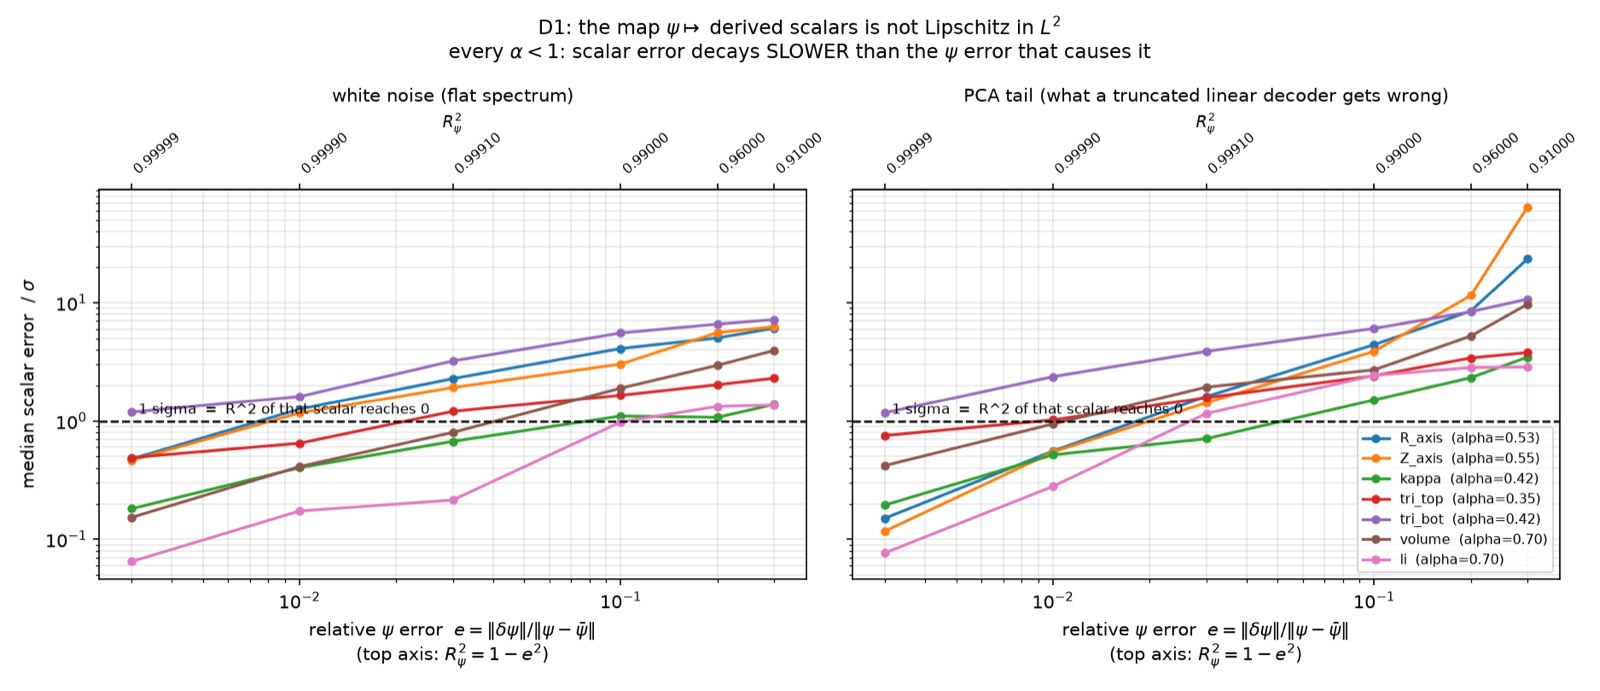
\includegraphics[width=\textwidth]{g02_amplification.jpg}
\caption{Медіанна похибка семи скалярів (у одиницях $\sigma_f$) проти відносної похибки
$\psi$; зліва --- білий шум, справа --- хвіст PCA. Пунктир --- $1\,\sigma$, де $R^2$ скаляра
падає приблизно до нуля; верхня вісь --- $R^2_\psi$. Власний розрахунок, код:
\texttt{Our try/03-deep-dives/D1-psi-to-scalars/\{conditioning,plots\}.py}.}
\label{fig:g02-amp}
\end{figure}

Для масштабу: Stokolesov та ін. \cite{Stokolesov2025} повідомляють середнє зміщення
0,04~м для LCFS DIII-D, відновленої лише зі струмів котушок. Наші 3,4--4,3~см при
$R^2_\psi=0{,}99$ --- той самий порядок, тобто числа фізично осмислені.

\paragraph{Що в цих числах варто читати обережно.} Реєстр подає їх чесно, але кілька
деталей видно лише у \texttt{results.json}:
\begin{itemize}
\item $\sigma_f$ пораховано лише по трьох розрядах. Для $\Rax$ це 8,9~мм --- третина
  ширини комірки сітки (26,6~мм), тож «$1\,\sigma$» тут --- субпіксельний зсув. Нормовані
  похибки через це виглядають більшими, ніж були б на повному корпусі. Але $\alpha$ --- нахил
  у логарифмічних координатах, і від $\sigma_f$ він не залежить: $\sigma_f$ зсуває лише
  перетин. Тому якісний висновок E1 стійкий, а абсолютні значення подано окремо.
\item Колонка «похибка при $R^2_\psi=0{,}99$» --- значення \emph{підгонки}, а не
  виміру: для $\Rax$ підгонка дає 3,76$\,\sigma$, а виміряна медіана при $e=0{,}1$ ---
  4,11$\,\sigma$. Для $\dlo$ точка $e^{*}=0{,}0022$ лежить \emph{нижче} найменшої виміряної
  амплітуди 0,003 (там медіана вже 1,19$\,\sigma$), тобто це екстраполяція.
\item E3 справджується при великих $e$, але не рівномірно: при $e=0{,}003$ хвіст PCA
  зсуває вісь \emph{менше} за білий шум ($\Rax$: 0,15 проти 0,48$\,\sigma$), при $e=0{,}1$ ---
  майже так само (4,4 проти 4,1$\,\sigma$), і лише далі різниця вибухає (при $e=0{,}3$:
  23,5 проти 6,1 для $\Rax$, 64,4 проти 6,3 для $\Zax$). Англійський підсумок реєстру
  «у 10 разів шкідливіший» --- це саме $e=0{,}3$. При $e=0{,}3$ хвіст PCA ще й ламає
  пошук LCFS у 7 зі 180 вимірів (\texttt{n}~= 173).
\end{itemize}
Чому хвіст PCA такий руйнівний при великих $e$, реєстр не пояснює. Правдоподібна
версія: компоненти хвоста --- це напрями, у яких кадри ансамблю \emph{справді} відрізняються
на дрібному масштабі, тобто вони зосереджені там, де $\psi$ змінюється від кадру до
кадру (біля осі й межі), а не розмазані по всій сітці, як білий шум. Це інтерпретація, не
вимір.

\paragraph{Спектральна крива і гіпотеза C2.} При фіксованій $\|\delta\psi\|$ ($e=0{,}1$)
різні скаляри бояться різних мод (рис.~\ref{fig:g02-spec}): об'єм і $\dup$ --- низьких
хвильових чисел $|k|=1\text{--}4$ (глобальна форма), $\Rax$ --- середніх ($|k|\approx6\text{--}9$),
$\Zax$ і $\li$ --- $|k|\approx9\text{--}13$ ($\li$ містить $|\grad\psi|^2$, тож підсилює
високі $k$); $\kappa$ майже нечутлива до $k$. Наслідок: пласка $L^2$-втрата на $\psi$ ---
не та цільова функція, і з кривої $S(k)$ можна вивести спектрально зважену. Це й було
гіпотезою C2; перевірка 2026-09-30 її \emph{спростувала} (п.~\ref{sec:g02-c2}).

\begin{figure}[ht]
\centering
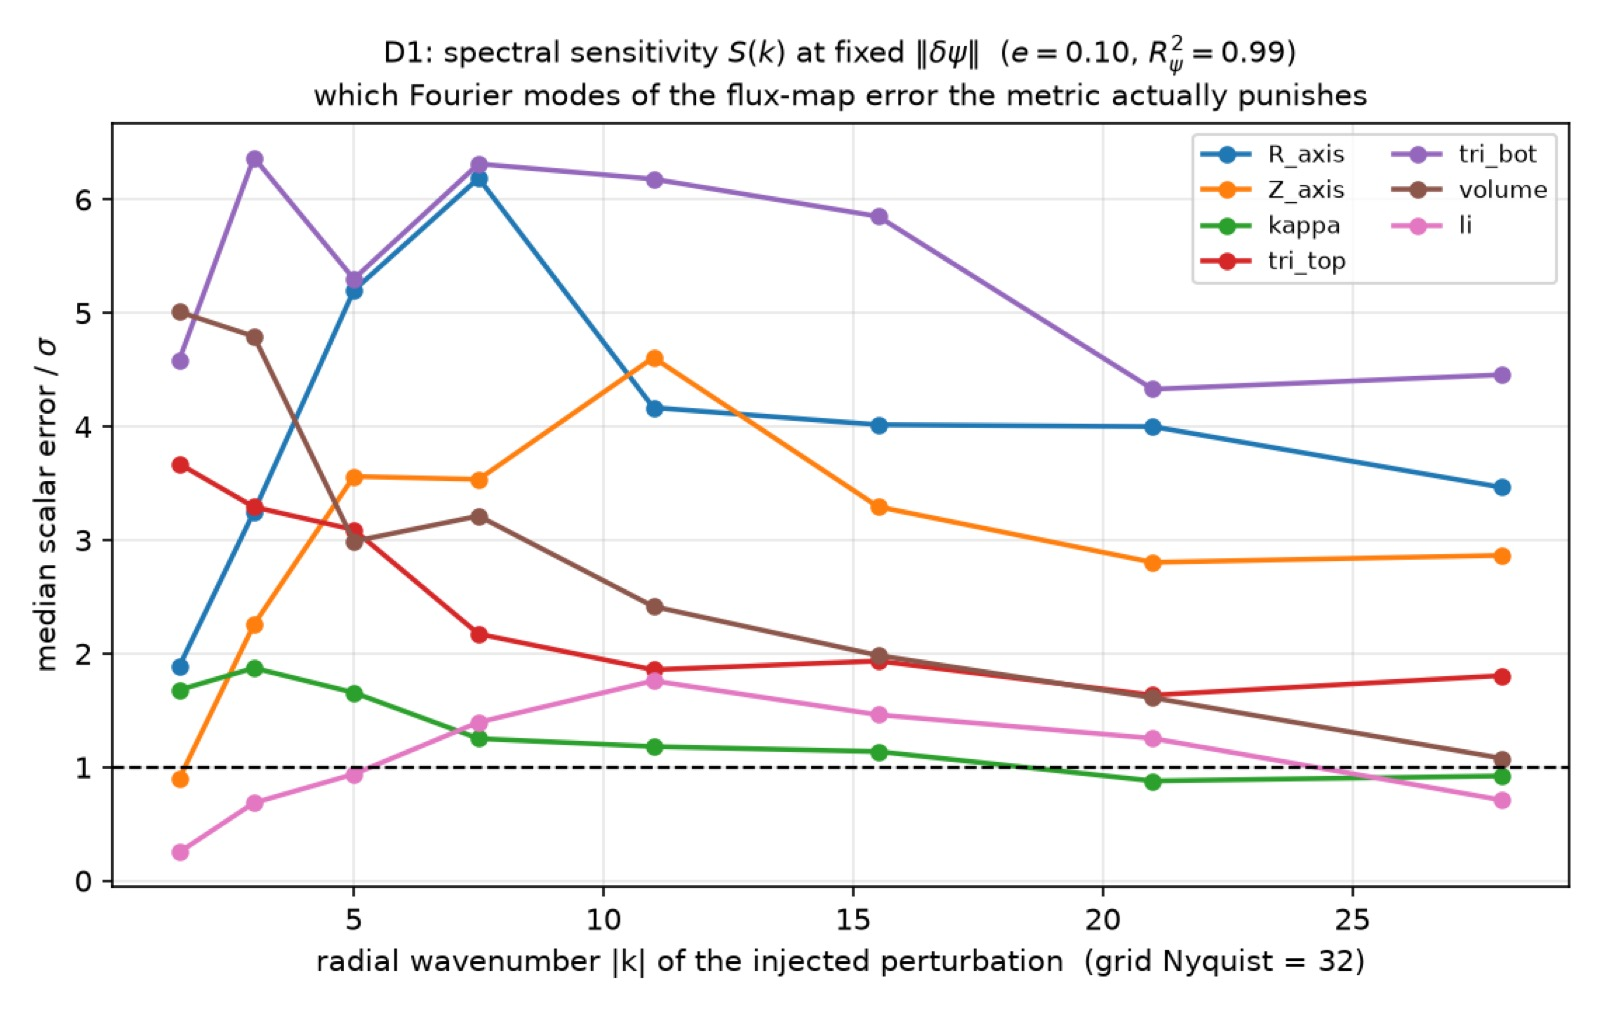
\includegraphics[width=0.72\textwidth]{g02_spectral_sensitivity.jpg}
\caption{Спектральна чутливість $S(k)$: медіанна похибка скалярів при збуренні в кільці
хвильових чисел, $e=0{,}10$ ($R^2_\psi=0{,}99$). Власний розрахунок, код:
\texttt{Our try/03-deep-dives/D1-psi-to-scalars/\{conditioning,plots\}.py}.}
\label{fig:g02-spec}
\end{figure}

Що з цього випливло для проєкту: якщо $R^2_\psi$ і Consistency розчіплюються так рано,
ще один $L^2$-член метрики нічого не лікує. Потрібна \emph{диференціальна} величина ---
нев'язка рівняння Ґреда--Шафранова, норма другого порядку, яка бачить саме ті моди, що
їх пропускає $L^2$. Це обґрунтування осі новизни №1 і рішення D6 (розд.~\ref{ch:g04}).
Декомпозиція похибки DeepONet \cite{Lanthaler2022} (кодування + апроксимація +
реконструкція) тут отримує уточнення: член реконструкції б'є не рівномірно, а по
найчутливіших напрямках --- принаймні при великих $e$.

\section{E14, R6 і C3: тест відновлено}\label{sec:g02-noscript}

До 2026-09-30 цей підрозділ називався «Пункти без відтворюваного коду»: синтетичний тест
2026-09-23 не зберегли (знахідка N5). Під час перевірки C1 його відновлено
(\texttt{c1/e14\_curvature.py}, \cite{RegEst,RegLog}).

\begin{itemcard}{E14}{встановлено (виміряно); \textbf{відтворено 2026-09-30}}
Зміщення осі під шумом $\propto1/\sqrt\lambda$ від кривизни: $|\Delta x|\sqrt\lambda$
стала в межах $\pm7\,\%$ на 16-кратному діапазоні $\lambda$. Відновлений тест дає для
$R$ при $\eta=10^{-2}$ і $\lambda=1\ldots16$ значення 0,0424--0,0474, тобто $\pm5{,}6\,\%$.
Умова --- режим стрибків, $\eta\gg\eta^{*}$. Для $Z$ за того самого $\eta$ закон не
виконується ($\pm19\,\%$): крок сітки по $Z$ --- 5~см, і для великих $\lambda$ режим стрибків
ще не настав.
\end{itemcard}
\begin{itemcard}{R6}{спростовано; \textbf{механізм відтворено 2026-09-30}}
«$\alpha=\tfrac12$ --- універсальний закон для положення критичної точки». Синтетика
2026-09-23 дала 0,687 при $\lambda=1$ і 0,841 при $\lambda=4$. Відновлений тест у
фіксованому вікні $\eta\in[10^{-5};10^{-2}]$ дає 0,746 / 0,819 / 0,884 / 0,938 / 0,976
для $\lambda=1,2,4,8,16$: $\alpha$ росте з $\lambda$, бо вікно захоплює дедалі більше
лінійного режиму. Точні числа 2026-09-23 не відтворюються --- вікно того тесту невідоме.
\end{itemcard}
\begin{conjecture}{C3}
Число обумовленості з E14 ($1/\sqrt\lambda$ в O-точці) корисне для стратифікації тесту.
\emph{Спростує:} розподіл $\lambda$ по корпусу виявиться вузьким --- стратифікувати нема за
чим. \emph{Стан 2026-09-30:} на 28 розрядах DIII-D $\lambda\in[0{,}13;\,3{,}6]$ (міжквартильний
розмах 0,73--1,58) --- розподіл широкий, тож головний спростовувач не спрацював. Але $\alpha$
осі між терцилями $\lambda$ змінюється слабко й непослідовно (0,47 / 0,54 / 0,54). Вердикту
ще немає \cite{RegConj}.
\end{conjecture}
\noindent Внутрішня напруга, про яку тут писало попереднє видання путівника («E14 каже
$1/\sqrt\lambda$ стала, а R6 --- що показник залежить від $\lambda$»), розв'язалася: обидва
твердження --- наслідки одного механізму E36, і тепер це перевіряється кодом.

\section{Перевірка C1 (2026-09-30): кластери --- властивість вибірки}\label{sec:g02-c1}

\paragraph{Навіщо.} Реєстр називав C1 найбазовішою гіпотезою розбору: якщо три кластери E2
справді відповідають трьом механізмам (екстремум, контур крізь сідло, інтеграл), D1 ---
теорія; якщо ні --- каталог чисел. \emph{Спростує:} синтетика з контрольованою геометрією дає
інші кластери, або кластери зникають при зміні вибірки розрядів \cite{RegConj}.

\paragraph{Як.} Спершу --- \emph{попередня реєстрація}: до будь-яких нових обчислень ми
записали в \texttt{c1/THEORY.md}, що саме рахує скорер для кожного скаляра, яке $\alpha$
очікуємо, що таке «кластер» (одновимірна k-means, силует $>0{,}5$) і за яких чисел C1
вважається підтвердженою чи спростованою. Туди ж записано конкурентну гіпотезу H-alt:
«положення екстремуму ($\Rax,\Zax$, а також $\dup,\dlo$ --- це $R$ у найвищій і найнижчій
точках контуру) дає $\approx\tfrac12$, а значення й інтеграли --- $\gtrsim0{,}8$». Далі чотири
кроки: відтворення D1; локальні моделі (параболоїд, «крапля» з X-точкою); 12 однонульових
рівноваг Серфона--Фрайдберга \cite{Cerfon2010} через увесь скорер; реальні дані --- 3 демо-розряди,
25 розрядів DIII-D з корпусу \cite{FEC} і 3 розряди MAST, з бутстрепом по \emph{розрядах}.

\code{ourtry/03-deep-dives/D1-psi-to-scalars/c1/alpha_tools.py}{149}{169}{(бутстреп по розрядах)}

\begin{itemize}
\item \emph{Рядки 152--153:} одиниця перевибірки --- розряд, а не кадр. Кадри одного розряду
  сильно корельовані, тож перевибірка кадрів дала б оманливо вузькі інтервали.
\item \emph{Рядки 158--161:} розряди витягаємо з поверненням, збираємо всі їхні кадри й
  перераховуємо медіанні криві та $\alpha$ тим самим \texttt{analyse}.
\item \emph{Рядки 162--169:} для кожної перевибірки записуємо $\alpha$ і розбиття семи
  скалярів на групи (найкраще за силуетом і примусово на три). Частка перевибірок, у
  яких розбиття збігається з C1, --- головне число вердикту.
\end{itemize}

\paragraph{Що вийшло.} Білий шум, $\alpha$ --- пряма через $e=0{,}003\ldots0{,}3$, як у D1;
частка 1000 перевибірок із розбиттям C1:
\begin{center}\small
\begin{tabular}{@{}lcc@{}}
\toprule
вибірка & відмінність від E2 & розбиття C1 \\
\midrule
DIII-D, 3 демо-розряди (як у D1) & --- & 96,7\,\% \\
DIII-D, 28 розрядів & $\li$: 0,70 $\to$ 0,47 (в інтервалі осі) & \textbf{0\,\%} \\
MAST, 3 розряди & $\Zax$: 0,55 $\to$ 0,71 & 3,3\,\% \\
Серфон--Фрайдберг, 12 форм & $\li$ 0,92, $\kappa$ 0,57 & 0,3\,\% \\
\bottomrule
\end{tabular}
\end{center}
Для гладкого збурення ($|k|<4$) усі $\alpha\approx0{,}69\text{--}1{,}08$, і кластерів немає ніде.
H-alt теж не пройшла (0--1,2\,\%).

\begin{figure}[ht]
\centering
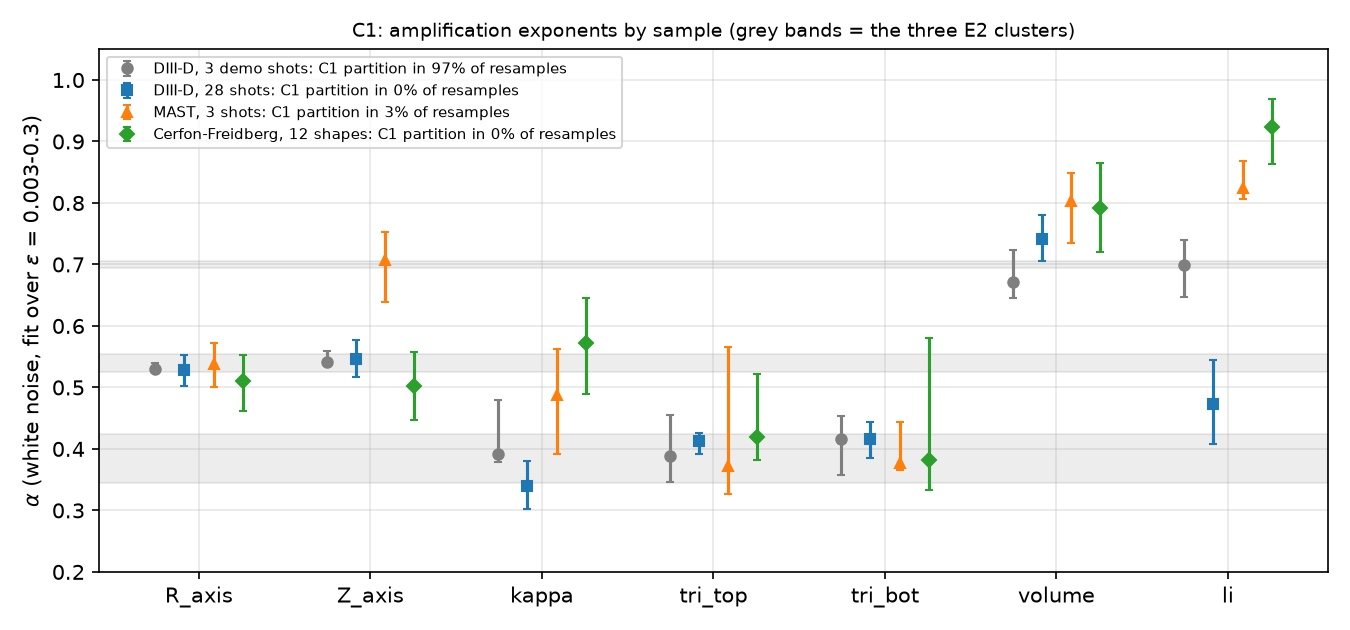
\includegraphics[width=\textwidth]{g02_c1_alpha_samples.jpg}
\caption{Показники $\alpha$ (білий шум, оцінювач D1) для чотирьох вибірок із 95\,\% бутстреп-інтервалами;
сірі смуги --- три кластери E2. Власний розрахунок, код:
\texttt{Our try/03-deep-dives/D1-psi-to-scalars/c1/\{real\_sweep,cf\_xpoint,summarise\}.py}.}
\label{fig:g02-c1-samples}
\end{figure}

\begin{refuted}{R10 (була гіпотеза C1)}
«Три кластери $\alpha$ відповідають трьом механізмам». Розбиття стабільне лише на трьох
демо-розрядах, на яких його й побачили; на 28 розрядах DIII-D, на MAST і на синтетиці його
немає (0--3,3\,\%). Спростовано за критеріями, записаними до запуску \cite{RegEst}.
\end{refuted}

\paragraph{Що встановлено натомість.} Механізм для осі з рамки «Виведення» (п.~\ref{sec:g02-physics})
перевірено на параболоїді з кривиною $\lambda=1\ldots16$ на сітці DIII-D. Вісь шукає сама функція
скорера \texttt{find\_o\_point}.

\code{ourtry/03-deep-dives/D1-psi-to-scalars/c1/local_models.py}{50}{68}{(тест P1 / E14)}

\begin{itemize}
\item \emph{Рядки 57--61:} центр параболоїда випадково зсунуто в межах півкроку сітки --- інакше
  максимум завжди сидів би точно у вузлі, і параболічне уточнення нічого б не показало.
\item \emph{Рядки 62--64:} той самий генератор дає або білий шум (незалежний у кожному
  вузлі), або гладкий ($|k|<4$, нормований на ту саму амплітуду у вузлі); вісь
  шукає функція скорера до і після збурення.
\item \emph{Рядки 65--68:} медіана зсуву по 300 спробах для кожного $\eta$. Наступний
  рядок (поза фрагментом) рахує з цих медіан локальні нахили між сусідніми $\eta$.
\end{itemize}

\begin{figure}[ht]
\centering
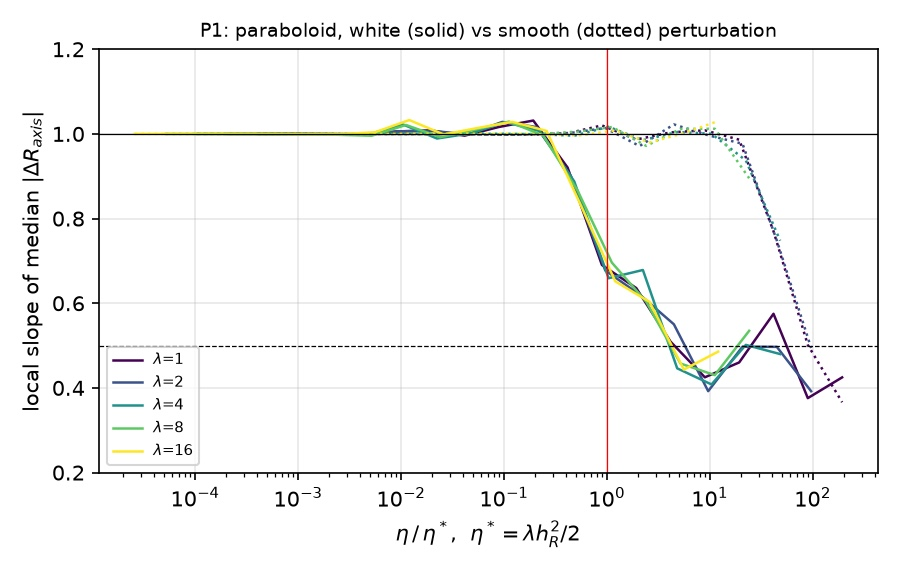
\includegraphics[width=0.72\textwidth]{g02_c1_m1_crossover.jpg}
\caption{Локальний нахил медіанного $|\Delta\Rax|$ проти $\eta/\eta^{*}$, $\eta^{*}=\lambda h_R^2/2$:
суцільні --- білий шум, пунктир --- гладке збурення; кольори --- $\lambda=1\ldots16$. Власний
розрахунок, код: \texttt{c1/local\_models.py}, \texttt{c1/summarise.py}.}
\label{fig:g02-c1-m1}
\end{figure}

\begin{established}{E36}
Для білого шуму нахил похибки осі дорівнює 1, поки $\eta<\eta^{*}=\lambda h^2/2$ (параболічне
уточнення лінійне), і $\approx0{,}4\text{--}0{,}5$, коли $\eta\gtrsim\eta^{*}$ (дискретний
максимум стрибає). Криві для різних $\lambda$ лягають на одну в координатах $\eta/\eta^{*}$.
Для гладкого збурення нахил 1. Звідси $\alpha\approx\tfrac12$ осі в D1 --- режим стрибків на
сітці, а R6 --- наслідок фіксованого вікна $\eta$ \cite{RegEst}.
\end{established}

\paragraph{Що лишилося відкритим.} (1)~$\li$ на 28 реальних розрядах має $\alpha=0{,}47$, а на
синтетиці $\approx0{,}92\text{--}0{,}97$: на реальних кадрах $\li$ чутливе до чогось, чого немає в
рівновагах Соловйова. (2)~$\dup,\dlo$ дають $0{,}34\text{--}0{,}42$, нижче передбаченої $\tfrac12$;
імовірна причина --- $R$ береться в \texttt{argmax}~$Z$ серед 512 точок контуру, тобто змінюється
стрибками. (3)~Хвіст PCA на 28 розрядах дає розбиття C1 у 100\,\% перевибірок, але на MAST і
синтетиці --- ні; базис PCA сам залежить від вибірки, тож це спостереження, а не підтримка C1.

\section{Перевірка C2 (2026-09-30): вага не лікує розчеплення}\label{sec:g02-c2}

\paragraph{Що стверджувалось.} C2: спектрально зважена втрата, виведена з кривої $S(k)$, покращує
реальні моделі. \emph{Спростує:} бейзлайн, навчений із нею і без неї, має однаковий $S'$
\cite{RegConj}. $S'$ ще не реалізовано (член Calibration потребує невизначеності), тож до запуску
мірою записали \textbf{Consistency} (головна) і композитний \textbf{S} офіційного скорера.

\paragraph{Як.} Як і для C1, спершу --- попередня реєстрація (\texttt{c2/THEORY.md}): правило
виведення ваги, три контролі й критерії. Потім:
\begin{itemize}
\item $S(k)$ переміряно на 28 розрядах. У робочій точці моделей крива майже монотонно спадає
  з~$k$: найшкідливіші \emph{низькі} хвильові числа, а не середні, як у D1 при $e=0{,}1$.
\item Робоча точка: пласка PCA+Ridge на валідаційних розрядах має $R^2_\psi=0{,}940$, тобто
  $e_{\mathrm{op}}=0{,}245$; береться $S(k)$ при $e=0{,}3$. Ваги кілець спадають від 0,91 до 0,49.
\item Чотири «руки»: пласка MSE; вага $S(k)$; вага $H^1$ ($1+(k/k_c)^2$ з тим самим діапазоном,
  але зростаюча); ті самі числа $S(k)$, переставлені випадково.
\item Моделі: PCA+Ridge (вага діє через зважену PCA) і UNet\_Lite зі стартового набору (вага
  прямо у втраті, 3 зерна). Розбиття --- як у \texttt{SCORE.md}: навчання на потокових розрядах
  0--35, валідація 36--39, тест 60--67.
\end{itemize}

\code{ourtry/03-deep-dives/D1-psi-to-scalars/c2/train.py}{116}{127}{(зважена втрата у просторі Фур'є)}

\begin{itemize}
\item \emph{Рядки 121--123:} \texttt{rfft2} зберігає лише половину спектра дійсного поля, тож
  стовпці 1--32 входять удвічі (їхні спряжені пари не записано). Ділення на $(N^2)^2$ за
  рівністю Парсеваля робить пласку вагу $w\equiv1$ точно рівною звичайній MSE.
\item \emph{Рядки 125--127:} втрата --- зважена сума $|\widehat{\delta\psi}(k)|^2$. Та сама
  функція працює для всіх чотирьох рук, змінюється лише масив \texttt{w}: різниця між руками
  --- тільки у вазі, а не в коді.
\end{itemize}

\paragraph{Що вийшло.} Вісім тестових розрядів, UNet\_Lite --- середнє трьох зерен, 95\,\%
інтервали --- бутстреп по розрядах:
\begin{center}\small
\begin{tabular}{@{}llccc@{}}
\toprule
модель & вага & Consistency & $\Delta$ до flat [95\,\% ДІ] & $R^2_\psi$ \\
\midrule
PCA+Ridge & усі чотири & 0,2698 & $|\Delta|<10^{-4}$ & 0,090 \\
UNet\_Lite & flat & 0,179 & --- & 0,976 \\
UNet\_Lite & $S(k)$ & 0,168 & $-0{,}011$ [$-0{,}044$; $+0{,}012$] & 0,976 \\
UNet\_Lite & $H^1$ & 0,162 & $-0{,}017$ [$-0{,}070$; $+0{,}012$] & 0,975 \\
UNet\_Lite & shuffled & 0,177 & $-0{,}002$ [$-0{,}049$; $+0{,}019$] & 0,975 \\
\bottomrule
\end{tabular}
\end{center}

\begin{figure}[ht]
\centering
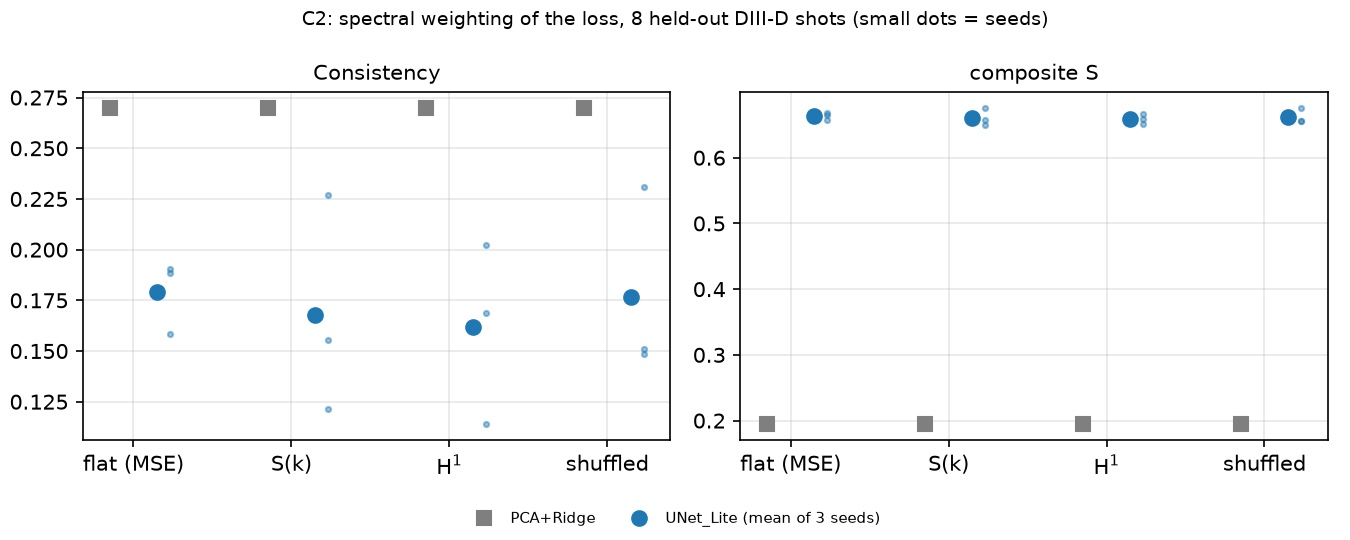
\includegraphics[width=\textwidth]{g02_c2_arms.jpg}
\caption{Consistency і композитний S для двох моделей і чотирьох вагових схем; дрібні точки ---
окремі зерна UNet\_Lite. Власний розрахунок, код:
\texttt{Our try/03-deep-dives/D1-psi-to-scalars/c2/\{train,evaluate,summarise\}.py}.}
\label{fig:g02-c2}
\end{figure}

PCA+Ridge на вагу не реагує: вага змінює лише базис PCA, а 50 компонент зважених і незважених
даних охоплюють майже той самий простір. У UNet\_Lite жодна вага не допомогла, а розкид між
зернами (Consistency від 0,114 до 0,231) більший за будь-яку різницю між руками
(рис.~\ref{fig:g02-c2}).

\begin{refuted}{R11 (була гіпотеза C2)}
«Спектрально зважена втрата, виведена з $S(k)$, покращує реальні моделі». Для обох моделей
інтервал $\Delta$Consistency містить нуль; $S(k)$ не краща ні за $H^1$, ні за перемішану вагу.
Спростовано за критеріями, записаними до навчання \cite{RegEst}.
\end{refuted}

\begin{established}{E37}
Розчеплення $R^2_\psi$ і Consistency видно й на навченій моделі. На тих самих восьми розрядах
UNet\_Lite має $R^2_\psi=0{,}976$, але Consistency лише 0,179 ($R^2$ для $\Zax$ дорівнює $-1{,}92$,
для $\kappa$ --- $-1{,}39$). У PCA+Ridge карта потоку майже марна ($R^2_\psi=0{,}090$), а
Consistency вища --- 0,270. Це теза E1, перевірена вже не штучними збуреннями \cite{RegEst}.
\end{established}

\paragraph{Що з цього випливає.} Перерозподіл $L^2$-похибки за хвильовими числами розчеплення не
лікує. Логічний наступний крок --- пряма мета на скаляри або диференціальний член (нев'язка ГШ),
тобто гіпотеза C4 (розд.~\ref{ch:g04}). \emph{Застереження:} одна архітектура, три зерна, вісім
тестових розрядів; діапазон ваг лише $1{,}85\times$ --- сильніша вага не перевірялась.

\section{Гіпотези і завдання}\label{sec:g02-tasks}

\begin{practicum}[R10, R11, C3 своїми руками]
\begin{enumerate}
\item \textbf{Відтворення.} У теці стартового набору:
  \texttt{.venv/bin/python "../../Our try/03-deep-dives/D1-psi-to-scalars/conditioning.py"
  --frames 60 --seeds 3 --out /tmp/d1} і порівняйте \texttt{/tmp/d1/results.json} з
  оригіналом (\texttt{--out} не дасть перезаписати файл проєкту).
\item \textbf{R10: відтворення.} Команди --- у \texttt{c1/README.md} (близько 6~хв на
  8 ядрах). Звірте частки розбиття C1 з таблицею п.~\ref{sec:g02-c1}.
\item \textbf{Загадка $\li$.} Чому на реальних кадрах $\alpha(\li)=0{,}47$, а на синтетиці
  $\approx0{,}95$? Порівняйте, де в кадрі лежить LCFS (сідло чи дотик до маски) і як часто
  вона перескакує під шумом. Сирі похибки є в \texttt{c1/real\_sweep\_DIII-D.npz}.
\item \textbf{Дискретність $\dup,\dlo$.} Замініть у копії \texttt{derive.\_shape\_from\_contour}
  \texttt{argmax} на параболічне уточнення вершини контуру. Чи підніметься $\alpha$ до $\tfrac12$?
\item \textbf{C3.} Кривизну $\lambda$ в O-точці для кожного кадру вже рахує
  \texttt{c1/real\_sweep.py} (\texttt{axis\_curvature}); розподіл широкий. Наступний крок ---
  стратифікувати за $\lambda$ не синтетичний шум, а залишки справжнього бейзлайну PCA+Ridge.
\item \textbf{R11: сильніша вага.} У \texttt{c2/train.py} візьміть $S(k)$ при $e=1{,}0$
  (діапазон ваг більший) або піднесіть ваги до степеня 3. Чи з'явиться ефект, більший за розкид
  між зернами? Скільки зерен потрібно, щоб його побачити?
\item \textbf{E37: пряма мета на скаляри.} Додайте до UNet\_Lite другу голову, що прогнозує сім
  скалярів Consistency (їхні еталонні значення рахує \texttt{local\_score.build\_reference}).
  Чи зросте Consistency, і чим доведеться заплатити в $R^2_\psi$?
\end{enumerate}
\end{practicum}

\chapter{Бін \texorpdfstring{$\neq$}{≠} плазма, але корисний контроль}\label{ch:g03}

Це розділ про найповчальніше спростування проєкту. Ми висунули красиву гіпотезу про
спільну математику надпровідників і плазми, перевірили її --- і вона впала. Але те, що
лишилося після падіння, дало точний числовий результат, якого в літературі, наскільки
нам відомо, немає: середнє двох розв'язків нелінійної задачі не є розв'язком, і метрика
$L^2$ цього не бачить. Ланцюжок: R2~→ D8~→ E4/E5~→ C7 (рис.~\ref{fig:g00-chains}).

\section{Гіпотеза, яка впала: R2}\label{sec:g03-r2}

Пропозиція (2026-09-22, \texttt{Our try/02-field-map/D-superconductivity.md}) звучала так:
критичний стан Біна в надпровіднику II роду і задача Ґреда--Шафранова з вільною межею
мають спільну структуру «вільна межа~/ варіаційна нерівність», тож той самий чисельний
апарат (Deep Ritz, PINN, варіаційні розв'язувачі) застосовний до обох.

\begin{outofcorpus}[критичний стан Біна (плита, стале $J_c$)]
У моделі Біна густина струму в надпровіднику або дорівнює критичній, $|J|=J_c$, або
нульова. Для плити в паралельному полі $H_a$ профіль поля всередині
\[
H(x)=\max\bigl(H_a-J_c x,\;0\bigr),
\]
фронт проникнення $x_p=H_a/J_c$. Задача --- варіаційна нерівність з \emph{опуклою}
множиною обмежень $K=\{\,|{\pa H}/{\pa x}|\le J_c\,\}$; вільна межа --- це межа
\emph{активної множини}, де обмеження насичене.
\end{outofcorpus}

Перевірка літератури дала три факти, які вирішують справу \cite{RegEst,RegDec}:
\begin{enumerate}
\item \textbf{Опуклість.} Для сталого $J_c$ Прігожин \cite{Prigozhin1996} (Теорема~2)
  переписує задачу Біна як $\dd h/\dd t+\pa I_K(h)\ni f$, де $\pa I_K$ --- субдиференціал
  індикатора опуклої множини, максимально монотонний оператор. Звідси існування й
  \emph{єдиність}. Задача плазми --- напівлінійна нелінійна задача на власні значення з
  \emph{неопуклим} функціоналом; розв'язок у загальному випадку неєдиний \cite{Schaeffer1977,Bartolucci2021}.
\item \textbf{Перешкода проти лінії рівня.} У Біна вільна межа --- межа активної множини
  обмеження-нерівності з множником Лагранжа $\rho\ge0$. У плазми вона --- лінія рівня
  розв'язку $\pa\{v>0\}$: жодної перешкоди, жодного множника при нерівності.
\item \textbf{Нульове перехресне цитування за 50 років:} дві зрілі спільноти одна одну не
  цитують.
\end{enumerate}

\begin{established}{E24 (прочитано)}
Критичний стан Біна опуклий і однозначно розв'язний; задача плазми неопукла й
багатозначна (Prigozhin 1996, Тм.~2; Bartolucci та ін. 2021; Schaeffer 1977) \cite{RegEst}.
\end{established}
\begin{refuted}{R2}
«Критичний стан Біна і вільна межа плазми --- одна математика». Спростовано: опукла
проти неопуклої; активна множина проти лінії рівня; нульове перехресне цитування
\cite{RegEst}. Важливе застереження з огляду: PINN застосовні до обох задач --- але вони
застосовні майже до будь-якого PDE, і спільна застосовність універсального методу не є
доказом спільної структури.
\end{refuted}

\paragraph{Що врятували: D8.} Питання «чи це одна задача» замінили іншим: \emph{чи
відрізняється режим відмови методу між опуклою задачею з вільною межею і неопуклою?}
Бін стає \textbf{опуклим контролем}, проти якого видно наслідки неопуклості. Рішення D8
закрило надпровідність як окрему тему (2026-09-22) і злило її з глибоким розбором D2
\cite{RegDec}. Реєстр гіпотез прямо називає R2 одним із двох спростувань, які дали
\emph{кращий} результат, ніж містили.

\section{Навіщо неєдиність: аргумент проти \texorpdfstring{$L^2$}{L2}}\label{sec:g03-why}

\begin{established}{E21 (прочитано)}
Розв'язок рівняння Ґреда--Шафранова може бути неєдиним на реальній геометрії: Ham і
Farrell 2024 \cite{HamFarrell2024}; Pentland та ін. 2025 \cite{Pentland2025} (MAST-U,
дефляційна континуація) \cite{RegEst}.
\end{established}
\noindent Робота по MAST-U не містить машинного навчання взагалі, але містить потрібний
нам факт: коли підгонку обмежують лише магнітні виміри, дві дуже різні форми профілю
можуть давати однаковий потік на осі. Тобто відображення «діагностики~→ $\psi$», яке
вчить кожна ML-модель реконструкції, може бути не функцією, а \emph{багатозначним
відношенням}.

Регресор, що мінімізує $\mathbb{E}\|f(x)-y\|^2$, збігається до умовного середнього
$\mathbb{E}[y\,|\,x]$. Якщо за тих самих $x$ існують дві гілки $y_1,y_2$, модель
повертає щось на кшталт $\tfrac12(y_1+y_2)$. Для лінійного рівняння це теж розв'язок.
Для нелінійного --- ні, і ось чому.

\begin{derivation}[нев'язка середнього двох гілок]
Нехай $u_1,u_2$ розв'язують $u''+\lambda\ee^{u}=0$. Для
$\bar u=\tfrac12(u_1+u_2)$ маємо $\bar u''=-\tfrac{\lambda}{2}(\ee^{u_1}+\ee^{u_2})$, тож
\begin{equation}\label{eq:g03-jensen}
r[\bar u]\equiv\bar u''+\lambda\ee^{\bar u}
=\lambda\Bigl(\ee^{\bar u}-\tfrac12\bigl(\ee^{u_1}+\ee^{u_2}\bigr)\Bigr)\le0 .
\end{equation}
Нерівність --- це нерівність Єнсена для опуклої $\ee^{u}$; рівність лише при $u_1=u_2$.
Отже, середнє порушує рівняння \emph{всюди}, де гілки різні, і тим сильніше, чим далі
вони одна від одної. А в $L^2$ середнє --- найкраща можлива відповідь \emph{за
означенням}: жодне збільшення ваги $L^2$-члена цього не виявить. Для рівняння
Ґреда--Шафранова $\GSop\psi=-\mu_0R^2p'(\psi)-FF'(\psi)$ механізм той самий: права
частина нелінійна за $\psi$ (\cite{Manual}, розд.~3).
\end{derivation}

\section{Сурогат механізму: Братý проти Біна}\label{sec:g03-bratu}

Для точного експерименту потрібна неопукла задача, чиї гілки відомі в замкненій формі.
Такою є одновимірна задача Братý (Гельфанда)
\begin{equation}\label{eq:g03-bratu}
-u''=\lambda\ee^{u},\qquad u(0)=u(1)=0 .
\end{equation}
Bartolucci та ін. \cite{Bartolucci2021} відносять задачу плазми з вільною межею саме до
сімейства Гельфанда~/ середньопольових вихорів~/ напівлінійних біфуркацій, тож це
правильний родич, хоча й не сама GS.

\begin{outofcorpus}[гілки Братý і точка складки]
Розв'язок \eqref{eq:g03-bratu} має вигляд
$u(x)=-2\ln\bigl[\cosh(s\theta/2)/\cosh(\theta/4)\bigr]$, $s=x-\tfrac12$, де $\theta$
задовольняє $\theta=\sqrt{2\lambda}\cosh(\theta/4)$. Функція $\theta/\cosh(\theta/4)$ спершу
зростає, потім спадає, тож при $\lambda<\lambda^{*}$ рівняння має рівно два корені (дві
гілки), при $\lambda=\lambda^{*}$ --- один, далі жодного. Це \emph{складка} (fold). У точці
складки похідна $\theta/\cosh(\theta/4)$ нульова: $\cosh(\theta_c/4)=(\theta_c/4)\sinh(\theta_c/4)$,
$\lambda^{*}=\theta_c^2/\bigl(2\cosh^2(\theta_c/4)\bigr)$. Енергія
$J[u]=\int_0^1\bigl(\tfrac12u'^2-\lambda\ee^{u}\bigr)\dd x$ знаконевизначена й необмежена
знизу (візьміть $u=t\varphi$, $t\to\infty$); нижня гілка --- її локальний мінімум,
верхня --- сідлова точка («гірський перевал»).
\end{outofcorpus}

Контроль --- плита Біна зі сталим $J_c$: один розв'язок на кожне $H_a$, тож «умовне
середнє по множині розв'язків» просто збігається з розв'язком.

\subsection{Код: точні гілки}

\code{ourtry/03-deep-dives/D2-gs-nonuniqueness/branch_mean.py}{61}{83}{(корені $\theta$, гілки, точка складки)}

\begin{itemize}
\item \emph{Рядки 61--70, \texttt{theta\_roots}:} шукаємо обидва корені
  $g(\theta)=\theta-\sqrt{2\lambda}\cosh(\theta/4)$. Замість «вгадування» дужок --- густа
  сітка з 200\,000 точок на $[0,60]$, зміни знака $g$ і уточнення кожного кореня методом
  Брента (\texttt{brentq}) до $10^{-14}$. При $\lambda>\lambda^{*}$ змін знака немає ---
  список порожній.
\item \emph{Рядки 73--75, \texttt{bratu\_u}:} точна формула гілки для даного $\theta$.
\item \emph{Рядки 78--83, \texttt{lam\_star}:} точка складки з умови
  $\cosh(\theta/4)=(\theta/4)\sinh(\theta/4)$ --- знову \texttt{brentq}, потім
  $\lambda^{*}=\theta_c^2/(2\cosh^2(\theta_c/4))$. Це і є валідація реалізації (E5).
\end{itemize}

\subsection{Код: нев'язки}

\code{ourtry/03-deep-dives/D2-gs-nonuniqueness/branch_mean.py}{86}{104}{(профіль Біна, друга похідна, нев'язка Братý)}

\begin{itemize}
\item \emph{Рядки 87--89, \texttt{bean\_H}:} точний профіль Біна $\max(H_a-J_cx,0)$.
\item \emph{Рядки 93--97, \texttt{d2}:} друга похідна четвертого порядку точності
  (п'ятиточковий шаблон) на сітці з $N=20\,001$ вузла; крайні два вузли --- \texttt{NaN}.
\item \emph{Рядки 100--104, \texttt{rel\_residual\_bratu}:} відносна нев'язка
  $\|u''+\lambda\ee^{u}\|/\|\lambda\ee^{u}\|$ --- у частках норми джерела, з відступом
  200 вузлів від країв. Значення 1 означає, що нев'язка такого самого розміру, як сам
  член рівняння.
\end{itemize}

\code{ourtry/03-deep-dives/D2-gs-nonuniqueness/branch_mean.py}{107}{117}{(нев'язка Біна)}

\noindent \emph{Рядки 107--117:} для Біна перевіряємо $\dd H/\dd x+J_c=0$ лише в
проникненій області ($H>10^{-6}$), відступивши по 5 вузлів від країв і від злому на фронті;
сама вільна межа виключена. Нормування інше, ніж у Братý (на $J_c\sqrt n$), тож числа двох
задач порівнюємо за порядком, а не буквально.

\subsection{Код: експеримент}

\code{ourtry/03-deep-dives/D2-gs-nonuniqueness/branch_mean.py}{121}{145}{(неопуклий тест)}

\begin{itemize}
\item \emph{Рядки 122--124:} друкуємо $\lambda^{*}$ поруч із літературним 3,513830719.
\item \emph{Рядки 130--139:} для $\lambda\in\{0{,}5;\,1;\,2;\,3;\,3{,}4;\,3{,}5\}$ беремо обидві
  гілки, їхнє середнє \texttt{u\_mean} (те, що поверне $L^2$-регресор за рівноймовірних
  гілок) і три нев'язки.
\item \emph{Рядки 140--145:} \texttt{L2 sep} --- середньоквадратична відстань між гілками;
  усе пишеться в \texttt{rows}.
\end{itemize}

\code{ourtry/03-deep-dives/D2-gs-nonuniqueness/branch_mean.py}{147}{171}{(опуклий контроль і підсумок)}

\begin{itemize}
\item \emph{Рядки 149--158:} для п'яти значень $H_a$ «середнє по множині розв'язків» ---
  копія єдиного розв'язку (рядок 152).
\item \emph{Рядки 164--171:} головне порівняння: середня нев'язка справжньої гілки,
  середня нев'язка $L^2$-середнього (усереднено по шести $\lambda$) і те саме для Біна.
\end{itemize}

\section{Що вийшло}\label{sec:g03-results}

Прогін 2026-09-22 (\texttt{results.json}); функції \texttt{lam\_star}, \texttt{theta\_roots}
і нев'язки при $\lambda=0{,}5$ і $3{,}5$ ми 2026-09-29 перерахували імпортом модуля (без
запуску \texttt{main}, щоб не перезаписати файл) --- збіг до останньої цифри.

\begin{center}\small
\begin{tabular}{@{}ccccccc@{}}
\toprule
$\lambda$ & $\theta_{\mathrm{lo}}$ & $\theta_{\mathrm{hi}}$ & нев'язка (нижня) & нев'язка (верхня)
  & нев'язка середнього & відстань гілок \\
\midrule
0,5 & 1,0336 & 13,0382 & $3{,}40\cdot10^{-7}$ & $1{,}10\cdot10^{-8}$ & 4,2609 & 3,3624 \\
1,0 & 1,5172 & 10,9387 & $1{,}64\cdot10^{-7}$ & $1{,}26\cdot10^{-8}$ & 2,1018 & 2,6545 \\
2,0 & 2,3576 & 8,5072 & $7{,}22\cdot10^{-8}$ & $1{,}41\cdot10^{-8}$ & 0,7249 & 1,7514 \\
3,0 & 3,3735 & 6,5766 & $3{,}95\cdot10^{-8}$ & $1{,}63\cdot10^{-8}$ & 0,1745 & 0,9207 \\
3,4 & 4,1084 & 5,5623 & $2{,}94\cdot10^{-8}$ & $1{,}88\cdot10^{-8}$ & 0,0347 & 0,4193 \\
3,5 & 4,5519 & 5,0543 & $2{,}52\cdot10^{-8}$ & $2{,}37\cdot10^{-8}$ & 0,0041 & 0,1450 \\
\bottomrule
\end{tabular}
\end{center}

\begin{established}{E4}
$L^2$-середнє двох гілок не є розв'язком, і $L^2$ цього не бачить: відносна нев'язка
середнього \textbf{1,22} (середнє по шести $\lambda$) проти \textbf{$6{,}4\cdot10^{-8}$} у
справжньої гілки, тобто в $1{,}9\cdot10^{7}$ разів гірше; опуклий контроль Біна ---
\textbf{$2{,}5\cdot10^{-13}$} \cite{RegEst}.
\end{established}
\begin{established}{E5}
Реалізація валідна: точка складки Братý $\lambda^{*}=3{,}513830719$ збігається з
літературним значенням до останньої цифри ($\theta_c=4{,}7987$) \cite{RegEst}.
\end{established}

\begin{figure}[ht]
\centering
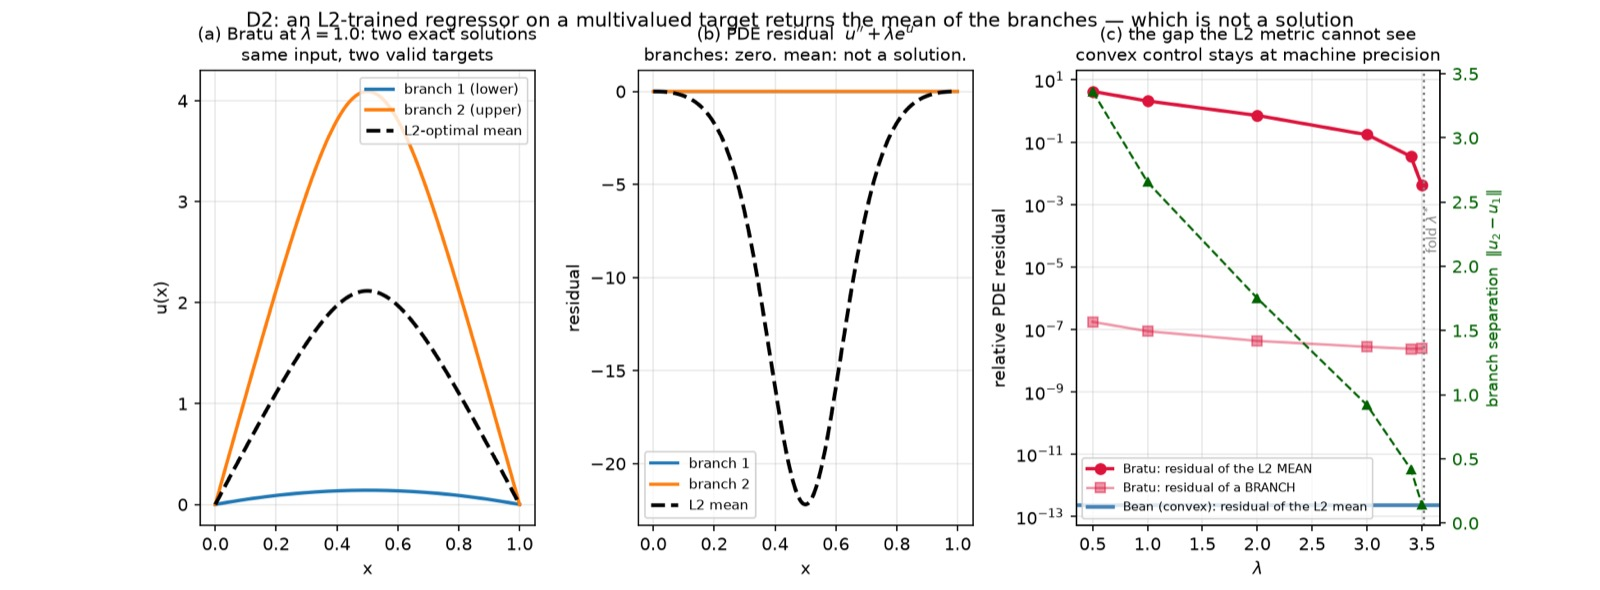
\includegraphics[width=\textwidth]{g03_branch_mean.jpg}
\caption{(a)~Дві точні гілки Братý при $\lambda=1$ і їхнє $L^2$-середнє; (b)~нев'язка
$u''+\lambda\ee^{u}$: у гілок нуль, у середнього --- від'ємна всюди, як
у~\eqref{eq:g03-jensen}; (c)~відносна нев'язка середнього і гілки проти $\lambda$, опуклий
контроль Біна і відстань між гілками (права вісь). Власний розрахунок, код:
\texttt{Our try/03-deep-dives/D2-gs-nonuniqueness/\{branch\_mean,plots\}.py}.}
\label{fig:g03-branch}
\end{figure}

Як це читати. Нев'язка 1,22 означає, що «розв'язок» порушує рівняння на величину порядку
самого джерела; при $\lambda=0{,}5$ --- учетверо більше. Структура залежності правильна:
при $\lambda\to\lambda^{*}$ гілки зливаються (відстань $3{,}36\to0{,}145$), і нев'язка
середнього падає до 0,0041, як і вимагає~\eqref{eq:g03-jensen}. Інформацію знищують не дані
і не потужність мережі: кожна окрема гілка має нев'язку на рівні числового шуму. Її знищує
\emph{цільова функція}. Правильні інструменти для багатозначних цілей відомі --- суміші
розподілів (MDN), умовні генеративні моделі, оборотні мережі.

\paragraph{Межі результату --- читати обов'язково.}
\begin{itemize}
\item Це \emph{не} Ґред--Шафранов. Перенесення висновку на GS спирається на цитати
  \cite{HamFarrell2024,Pentland2025,Bartolucci2021}, а не на цей розрахунок. Названий
  наступний крок --- дефляційна континуація поверх \texttt{FreeGSNKE} на геометрії MAST-U
  за рецептом Pentland та ін. --- не зроблено.
\item Контроль Біна в коді --- тавтологія: множина розв'язків одноелементна \emph{за
  побудовою} (рядок 152), тож рівність нев'язок розв'язку й «середнього» гарантована, а
  $2{,}5\cdot10^{-13}$ --- лише точність чисельної похідної кусково-лінійної функції. Уся
  змістовна частина контролю --- теорема Прігожина (E24); код її ілюструє, а не перевіряє.
\item Модель Біна--Кіма ($J_c$ залежить від поля) квазіваріаційна; для неї жодного
  аналогічного виміру немає.
\end{itemize}

\begin{itemcard}{Q3}{відкрите питання}
Чи неєдиність розв'язку GS (Ham--Farrell 2024, Pentland 2025) зустрічається в робочих
режимах, чи лише в екзотичних? Від цього залежить, чи розбір D2 --- реальна задача, чи
математичний курйоз. Адресат --- фізики плазми; статус --- відкрите \cite{RegQ}.
\end{itemcard}

\section{Наступний крок: C7 і Deep Ritz}\label{sec:g03-c7}

\begin{conjecture}{C7}
Deep Ritz на задачі плазми буде seed-нестабільним (обиратиме різні гілки), а на Біні ---
стабільним. \emph{Спростує:} обидва стабільні --- неопуклість не проявляється на доступних
масштабах. \emph{Вартість:} $\approx$ день, потрібні обидва розв'язувачі \cite{RegConj}.
\end{conjecture}

Метод Deep Ritz \cite{EYu2018} подає розв'язок нейромережею $u_\theta$ і мінімізує
енергію варіаційної задачі, оцінену Монте-Карло, плюс штраф за крайову умову. Приклад у
\texttt{Tokamak-GS-solver} --- загальний (десятивимірне рівняння Лапласа з точним
розв'язком $x_1x_2+x_3x_4+\ldots$), не GS і не Братý, але вся механіка на місці.

\code{gs/src/examples/deep_ritznet.py}{238}{259}{(цикл навчання Deep Ritz)}

\begin{itemize}
\item \emph{Рядки 241--243:} точки колокації всередині кулі (\texttt{data1}, з
  \texttt{requires\_grad}, бо знадобиться $\grad u$) і на межі (\texttt{data2}).
\item \emph{Рядки 246--250:} прямий прохід і $\grad u_\theta$ через
  \texttt{torch.autograd.grad} з \texttt{create\_graph=True} --- похідна має бути
  диференційовною за вагами.
\item \emph{Рядки 252--253:} енергія Рітца $\mathbb{E}\bigl[\tfrac12|\grad u|^2-fu\bigr]$ для
  $-\Delta u=f$ (тут $f=0$, функція \texttt{ffun}).
\item \emph{Рядки 256--259:} штраф $\beta\cdot$\,площа$\cdot\mathbb{E}(u-g)^2$ на межі
  ($\beta=500$) і повна втрата.
\end{itemize}
Зерно задано в рядку 327 (\texttt{torch.manual\_seed(21)}); саме його треба змінювати, щоб
міряти «дисперсію гілки по зернах».

\paragraph{Зауваження путівника до постановки C7.} Для Братý заміна \texttt{fTerm*output1}
на $\lambda\ee^{u}$ дає енергію $J[u]$, яка необмежена знизу (див. рамку вище). Чиста
мінімізація може знайти лише \emph{нижню} гілку (локальний мінімум) або «втекти» на
нескінченність; верхня гілка --- сідло, і градієнтний спуск її не обирає. Тому на Братý
C7 швидше проявиться як «збіжність до нижньої гілки або розбіжність залежно від зерна»,
ніж як вибір між двома гілками. Для справжньої задачі плазми Bartolucci та ін. мінімізують
на неопуклому многовиді зі сталою повного струму, і картина може бути іншою. Це
міркування, а не вимір; реєстр його не містить.

\begin{practicum}[C7: seed-стабільність Deep Ritz]
\begin{enumerate}
\item \textbf{Відтворення D2} (безпечно, у копії):
  скопіюйте \texttt{branch\_mean.py} і \texttt{plots.py} у власну теку й запустіть
  інтерпретатором стартового набору (розд.~\ref{sec:g00-run}); \texttt{results.json} має
  збігтися з наведеною таблицею.
\item \textbf{Контроль.} Одновимірна плита Біна з регуляризацією степеневим законом
  $E\propto(J/J_c)^n$ (опукла енергія). Deep Ritz на 10 зернах; міряйте положення фронту
  $x_p$ проти точного $H_a/J_c$. Очікування за E24: розкид мізерний.
\item \textbf{Тест.} Братý при $\lambda=1$: Deep Ritz на енергії $J[u]$ з 10 зернами. Для
  кожного зерна класифікуйте результат: нижня гілка ($u(\tfrac12)\approx0{,}141$),
  верхня ($u(\tfrac12)\approx4{,}091$; обидва значення --- з \texttt{bratu\_u}), розбіжність. Потім спробуйте варіант, що може знайти
  верхню гілку (наприклад, PINN на сильній нев'язці, де обидві гілки --- нулі втрати).
\item \textbf{Звіт у стилі реєстру:} що виміряно, чи спростовано C7 і в який бік; якщо
  результат --- «на Братý Deep Ritz бачить лише нижню гілку», це теж відповідь, і її треба
  записати, а не відкинути.
\end{enumerate}
\end{practicum}

\chapter{Нев'язка Ґреда--Шафранова як метрика}\label{ch:g04}

Чи можна оцінити передбачене поле $\psi(R,Z)$ не лише за тим, наскільки воно близьке до EFIT, а й за тим, чи є воно \emph{рівновагою} взагалі? У цьому розділі йдеться про пункти E6--E8, E22, E23, рішення D6 (метрика $S'$), гіпотези C4 і C6 та побічну знахідку E33. Фізику рівняння Ґреда--Шафранова (GS) див. у~\cite{Manual}, розд.~3, а реконструкцію рівноваги й машинне навчання~--- там само, розд.~12.

\section{Що не так з \texorpdfstring{$L^2$}{L2}: мотивація}\label{sec:g04-motivation}

Метрика Fusion Equilibrium Challenge (FEC)~\cite{FEC} зважує чотири члени: $R^2_\psi$, похідні скаляри $\qnf$ і $\betaN$, відстань між LCFS і Consistency (пулований $R^2$ семи похідних скалярів). Жоден із них не перевіряє, чи задовольняє поле фізичне рівняння. Три незалежні свідчення, що це не косметика, зібрано в \texttt{04-novelty/our-contribution.md}:

\begin{established}{E22 (прочитано)}
Мала $L^2$-похибка не гарантує малої фізичної нев'язки. У~\cite{Ding2025} суто керовані (supervised) моделі мали відносну $L^2$-похибку 0,25\,\% за великих нев'язок GS~\cite{RegEst}. Навчене відображення не є проєкцією Гальоркіна, тож стійкості на кшталт леми Сеа тут немає.
\end{established}

\begin{established}{E23 (прочитано)}
Жоден фузійний бенчмарк не оцінює нев'язку рівняння в частинних похідних (PDE). Поіменно перевірено FEC~\cite{FEC}, TokaMark~\cite{TokaMark2026}, PDEBench і The Well (журнал верифікації, V-A4~\cite{RegVerif}). Найближчий контрприклад~--- VEQDB (arXiv:2609.23296). Проте її «проєктований резидуал» (projected residual) міряє збіжність \emph{розв'язувача}, а не передбачення моделі. Окремі статті нев'язку звітують, тому твердження звужено до \emph{бенчмарків}: «бенчмарки оцінюють виходи, статті оцінюють фізику»~\cite{RegVerif}.
\end{established}

Третє свідчення наше: $L^2$-середнє двох гілок розв'язку GS має нев'язку 1,22 проти $6{,}4\cdot10^{-8}$ у справжньої гілки, і $L^2$-метрика цього не бачить за побудовою (E4, розд.~\ref{ch:g03}). З цього виросло рішення D6~\cite{RegDec}: метрика $S'$ дорівнює метриці FEC плюс GS-член плюс член калібрування невизначеності (UQ). Умова, за якої D6 переглядається: перевірка V-A4 покаже, що хтось уже оцінює нев'язку. Поки що не показала.

\section{Перешкода: у поданні немає \texorpdfstring{$p'$ і $FF'$}{p′ і FF′}}\label{sec:g04-obstacle}

Рівняння GS (\cite{Manual}, розд.~3) має вигляд
\begin{equation}\label{eq:g04-gs}
  \GSop\psi\equiv R\frac{\pa}{\pa R}\Big(\frac1R\frac{\pa\psi}{\pa R}\Big)+\frac{\pa^2\psi}{\pa Z^2}
  =-\mu_0R^2p'(\psi)-FF'(\psi).
\end{equation}
Команда подає лише $\psi$ на сітці $65\times65$. Профілів $p'$ і $FF'$ у поданні немає, тож наївну нев'язку обчислити не можна.

Вихід підказує сам EFIT~\cite{Lao1985}. Коли $\psi$ зафіксовано, праву частину \eqref{eq:g04-gs} можна розкласти за базисом поліномів від $\psiN$, і вона \emph{лінійна} за коефіцієнтами. Тому питання «чи є $\psi$ рівновагою?» зводиться до лінійних найменших квадратів (МНК): чи існує хоч якась пара функцій потоку, з якою \eqref{eq:g04-gs} виконується? Відносну нев'язку після найкращого підбору визначено в \texttt{04-novelty/metric-design.md}:
\begin{equation}\label{eq:g04-g}
  g(\psi)=\min_{\{a_i\},\{b_j\}}
  \frac{\big\|\GSop\psi+\sum_{i=0}^{n_p-1}a_iR^2\psiN^{\,i}+\sum_{j=0}^{n_f-1}b_j\psiN^{\,j}\big\|_{\Omega}}
       {\|\GSop\psi\|_{\Omega}},\qquad n_p=n_f=4 .
\end{equation}
Тут $\Omega$~--- пікселі всередині LCFS, крім двох крайових рядів і стовпців сітки. Коефіцієнти $a_i$ поглинають $\mu_0p'$, а $b_j$~--- $FF'$. Значення $g=0$ означає, що $\psi$ є рівновагою для деяких поліноміальних профілів.

\paragraph{Чому гладкістю це не обійти.} Умова \eqref{eq:g04-g} вимагає, щоб $\GSop\psi$ на кожній магнітній поверхні була афінною функцією $R^2$ з коефіцієнтами, що залежать лише від $\psi$. Це і є умова поверхні потоку. Гладке, але хибне поле її не виконує автоматично.

\section{Де це в коді}\label{sec:g04-code}

\code{ourtry/04-novelty/gs_residual_probe.py}{38}{61}{(оператор $\GSop$ і область плазми)}

\begin{itemize}
\item \textbf{Рядки 38--44} (\texttt{delta\_star}): $\GSop\psi=\pa_R^2\psi-R^{-1}\pa_R\psi+\pa_Z^2\psi$, центральні різниці другого порядку через \texttt{np.gradient}. Це розкритий вираз з \eqref{eq:g04-gs}: $R\,\pa_R(R^{-1}\pa_R\psi)=\pa_R^2\psi-R^{-1}\pa_R\psi$. Похідна береться двічі, тому похибка сітки підсилюється як $1/h^2$ (див.~\S\ref{sec:g04-physics}).
\item \textbf{Рядки 47--58} (\texttt{plasma\_mask}): LCFS видобувається \emph{тією самою} процедурою скорера (\texttt{extract\_lcfs}), що й для решти метрики. Точки всередині контуру знаходить \texttt{matplotlib.path}. Два крайові ряди й стовпці сітки відкидаються, щоб шаблон різниць не виходив за край. Зауважимо: до 2026-09-29 docstring обіцяв «ерозію на одну комірку», хоча код ерозії не робить, а лише обрізає край сітки; docstring виправлено 2026-09-29~\cite{RegLog}. Точки біля самої LCFS входять в $\Omega$.
\item \textbf{Рядки 59--61}: $\psiax$ береться в O-точці, $\psib$~--- як середнє по кожній восьмій точці контуру (білінійна інтерполяція \texttt{\_bilin}). З них отримуємо $\psiN$.
\end{itemize}

\code{ourtry/04-novelty/gs_residual_probe.py}{72}{86}{(найкращий МНК-підбір профілів)}

\begin{itemize}
\item \textbf{Рядки 74--76}: якщо LCFS не знайдено або в області менше 50 пікселів, повертається \texttt{nan}. Це чесне «не можу оцінити», а не нуль.
\item \textbf{Рядки 77--82}: стовпці матриці МНК~--- $R^2\psiN^{\,i}$ (відповідають $p'$) і $\psiN^{\,j}$ (відповідають $FF'$), по чотири кожного типу. $\psiN$ обрізано до $[0,1]$.
\item \textbf{Рядки 83--86}: \texttt{lstsq} розв'язує $A\,c\approx-y$, де $y=\GSop\psi$. Результат~--- відносна норма залишку $r=y+Ac$, тобто формула \eqref{eq:g04-g}.
\end{itemize}

\code{ourtry/04-novelty/gs_residual_probe.py}{106}{122}{(драбина збурень у \texttt{main})}

Рядки 106--115: для 12 рівномірно взятих кадрів розряду DIII-D 203702 обчислюємо $g$ на істині (EFIT) і на полях з білим шумом 1\,\% і 3\,\% від $\mathrm{std}(\psi)$. Зерно генератора дорівнює номеру кадру, тож прогін відтворюваний. Рядки 117--119 додають два контрольні варіанти: гаусове згладжування ($\sigma=1{,}5$ комірки) як «правдоподібне, але хибне» поле і масштаб $\psi\times1{,}05$ як вбудовану перевірку інваріантності.

\section{Що вийшло: E6--E8}\label{sec:g04-results}

\begin{established}{E6, E7, E8}
\textbf{E6.} GS-резидуал обчислюється лише з поданого $\psi$: на істині $g=0{,}009$, з 1\,\% шуму~--- 0,650 (у~70 разів більше), з 3\,\%~--- 0,921.
\textbf{E7.} Член інваріантний до масштабу: $\psi\times1{,}05$ значення не змінює.
\textbf{E8.} Член сліпий до гладкої похибки й до низькорангового усічення: гаусове згладжування дає 0,010, PCA-5~--- 0,0093 проти 0,009 на істині (було 0,016 без скрипта; уточнено в реєстрі 2026-09-29)~\cite{RegEst}.
\end{established}

Повторний запуск 2026-09-29 (\texttt{gs\_residual\_probe.py}, venv starter kit) дав такі медіани: істина 0,0092, шум 1\,\%~--- 0,6500, шум 3\,\%~--- 0,9207, згладжування 0,0095, масштаб 0,0092 (збігається з істиною до останнього знака). Числа E6, E7 і згладжування з E8 відтворились.

\emph{Розбіжність.} Рядка PCA-5 у цьому скрипті немає. Число 0,016 записано в \texttt{metric-\allowbreak design.md} і в E8, але скрипта, що його дає, у репозиторії не знайдено (ситуація та сама, що з E14, розд.~\ref{ch:g02}). Для путівника ми відновили перевірку тими самими функціями (\texttt{guide/\allowbreak figures/\allowbreak g04\_pca5\_check.py}): PCA-базис 166 скінченних кадрів розряду 203702, усічення до 5 компонент, ті самі 12 кадрів. Медіана вийшла $g=0{,}0093$, тобто ще ближче до істини. Висновок E8 («сліпий») тільки посилюється, але саме число 0,016 не відтворюється. Зареєстровано 2026-09-29 як уточнення E8: у реєстрі тепер 0,0093 (було 0,016 без скрипта), скрипт~--- \texttt{Our try/04-novelty/pca5\_check.py} (копія цього)~\cite{RegEst,RegLog}.

\section{Фізика: чому оператор другого порядку бачить те, чого не бачить \texorpdfstring{$L^2$}{L2}}\label{sec:g04-physics}

\begin{derivation}[спектральна вага нев'язки]
Нехай похибка передбачення~--- одна фур'є-гармоніка $\delta\psi=\varepsilon\,\ee^{\mathrm{i}\vect{k}\cdot\vect{x}}$ з $kR\gg1$. Тоді $\|\delta\psi\|_2\propto\varepsilon$, тоді як $\GSop\delta\psi\approx-k^2\delta\psi$ і $\|\GSop\delta\psi\|_2\propto k^2\varepsilon$. Отже, у нев'язці спектр похибки зважено множником $k^2$ (в енергії~--- $k^4$). Для білого шуму на сітці з кроком $h$ домінує $k\sim\pi/h$, тож шум 1\,\% у $\psi$ стає нев'язкою порядку одиниці (E6). Гладка похибка з $k\sim1/a$ (де $a$~--- малий радіус) має вагу в $(a/h)^2$ разів меншу. Крім того, вісім вільних коефіцієнтів МНК поглинають ту частину гладкого $\GSop\delta\psi$, яка лежить у їхній лінійній оболонці. Звідси сліпота до згладжування й усічення (E8).
\end{derivation}

\begin{derivation}[інваріантність до масштабу і знака]
Якщо $\psi$ розв'язує \eqref{eq:g04-gs} з профілями $p(\psi)$, $F(\psi)$, то $c\psi$ розв'язує його з $\tilde p(s)=c^2p(s/c)$, $\tilde F(s)=cF(s/c)$ (вправа 3 розд.~3 у~\cite{Manual}). Для самої нев'язки: $\GSop(c\psi)=c\,\GSop\psi$, $\psiN$ не змінюється, оптимальні коефіцієнти множаться на $c$, і відношення в \eqref{eq:g04-g} лишається тим самим. Отже, $g(c\psi)=g(\psi)$ за умови, що вісь і LCFS знайдено ті самі. Для $c>0$ це виконується автоматично (E7). Для $c=-1$ пошук осі й LCFS у скорері залежить від знакової конвенції машини і має запасний (fallback) шлях (розд.~\ref{ch:g06}), тож рівність треба перевірити. Інваріантність до знака важлива, бо DIII-D і MAST зберігають $\psi$ з протилежними знаками. У \texttt{metric-design.md} (перевірка 4) її виведено аналітично, але чисельно ще не перевірено.
\end{derivation}

Разом це дає чесний висновок \texttt{metric-design.md}. GS-член \emph{доповнює} $R^2_\psi$, а не замінює його: він ловить зернисті поля і середні гілок, тобто виходи, які взагалі не є рівновагами, але пропускає гладку похибку форми. У~\texttt{README.md} челенджу прямо записано, що нейронні бейзлайни дають карти потоку «глобально правильні, локально шорсткі». Саме таку відмову GS-член бачить безпосередньо.

\section{Метрика \texorpdfstring{$S'$}{S′} (D6)}\label{sec:g04-metric}

Пропозицію з \texttt{04-novelty/metric-design.md} наводимо без змін. Базова метрика FEC має вигляд
\[
  S=0{,}55\,R^2_\psi+0{,}15\,R^2_{\qnf,\betaN}+0{,}10\,(1-D_{\mathrm{LCFS}})+0{,}20\,\mathrm{Consistency},
\]
а запропонована~---
\begin{equation}\label{eq:g04-Sprime}
  S'=w_\psi R^2_\psi+w_{qb}R^2_{\qnf,\betaN}+w_L(1-D_{\mathrm{LCFS}})+w_c\,\mathrm{Consistency}
     +w_r\,\mathrm{GS}_{\mathrm{score}}+w_u\,\mathrm{Calibration},
\end{equation}
\begin{equation}\label{eq:g04-GSscore}
  \mathrm{GS}_{\mathrm{score}}=\mathrm{clip}\big(1-g/g_{\mathrm{ref}},\,0,\,1\big),\qquad g_{\mathrm{ref}}\approx0{,}10,
\end{equation}
\begin{equation}\label{eq:g04-calib}
  \mathrm{Calibration}=1-\frac{1}{|A|}\sum_{a\in A}\frac{|\mathrm{emp}(a)-a|}{\max(a,1-a)},\qquad A=\{0{,}5;\,0{,}8;\,0{,}9;\,0{,}95\}.
\end{equation}
Стартові ваги: $w_\psi=0{,}40$, $w_{qb}=0{,}10$, $w_L=0{,}10$, $w_c=0{,}15$, $w_r=0{,}15$, $w_u=0{,}10$. Ваги «потребують емпіричної перевірки, а не голосування». Значення $g_{\mathrm{ref}}$ підібрано так, щоб істина давала $\approx0{,}91$, а шум 1\,\%~--- нуль. Для надійного калібрування 12 кадрів одного розряду замало. З восьми обов'язкових самоперевірок у \texttt{metric-design.md} виконано лише одну (інваріантність до масштабу). Решта, зокрема \texttt{perfect}$\,\to1$, \texttt{zeros}$\,\to0$, геймабельність широкими смугами і поведінка на MAST, ще відкриті.

\section{C4: чи змінить \texorpdfstring{$S'$}{S′} упорядкування? Частковий результат}\label{sec:g04-c4}

\begin{conjecture}{C4}
Додавання $\mathrm{GS}_{\mathrm{score}}$ і Calibration змінить упорядкування семи наявних бейзлайнів. \emph{Спростує:} упорядкування за $S'$ збігається з упорядкуванням за $S$, тобто нові члени нічого не додають. \emph{Вартість:} близько півдня: реалізувати $S'$ і прогнати \texttt{experiments.py}~\cite{RegConj}. \emph{Стан 2026-10-01:} половину з $\mathrm{GS}_{\mathrm{score}}$ спростовано (R12, \S\ref{sec:g04-c4test}); частина про Calibration відкрита.
\end{conjecture}

Повної перевірки ще немає. Є частковий результат (N6, 2026-09), записаний у C4 з позначкою «не вердикт». Скрипт практикуму розд.~12 методички порівнює три поля: EFIT, прогноз бейзлайну PCA+Ridge і EFIT, стиснуте до 50 головних компонент тієї ж PCA.

\code{manualcode/ch11_gs_residual_baseline.py}{44}{59}{(три варіанти $\psi$ на 36 кадрах)}

Рядки 44--48 читають кожен демо-розряд DIII-D повністю і беруть прогноз бейзлайну (\texttt{bl.predict\_row}). Рядки 49--51 лишають кадри, скінченні в обох полях, і рівномірно вибирають 12 з них. Рядок 55 будує $L^2$-проєкцію на 50 компонент PCA самої моделі, тобто майже точне поле. Рядки 56--59 записують $R^2$ і $g$ для всіх трьох варіантів тією самою функцією \texttt{gs\_inconsistency}.

\begin{figure}[htbp]\centering
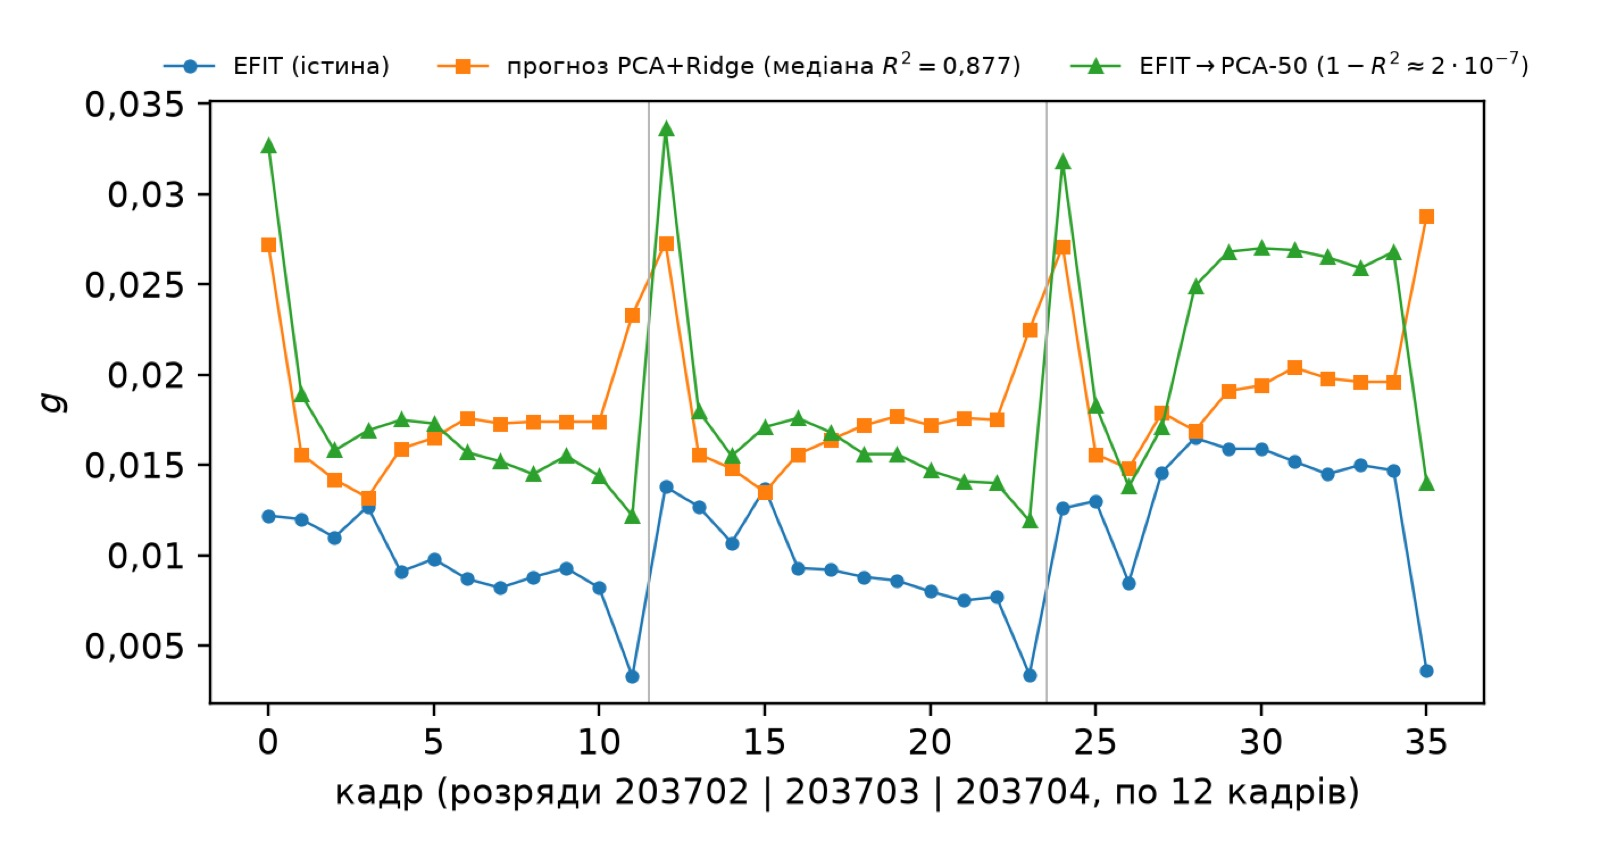
\includegraphics[width=0.92\textwidth]{g04_gs_residual.jpg}
\caption[GS-нев'язка на 36 кадрах DIII-D]{GS-нев'язка $g$ на 36 кадрах трьох демо-розрядів DIII-D для EFIT, прогнозу PCA+Ridge і PCA-50-проєкції EFIT. Власний розрахунок, код: \texttt{manual/code/ch11\_gs\_residual\_baseline.py} (прогін 2026-09-29), рисунок~--- \texttt{guide/figures/g04\_fig.py}. Дані: Fusion Equilibrium Challenge (Sophelio / General Atomics), CC BY 4.0.}\label{fig:g04-residual}
\end{figure}

Прогін 2026-09-29 відтворив медіани C4 до останнього знака: $g(\mathrm{EFIT})=0{,}0103$, $g(\text{прогноз})=0{,}0174$, $g(\text{PCA-50})=0{,}0170$. Медіана $R^2$ прогнозу 0,877, $1-R^2(\text{PCA-50})=2{,}26\cdot10^{-7}$; LCFS знайдено на всіх 36 кадрах. Звідси два спостереження (рис.~\ref{fig:g04-residual}):
\begin{enumerate}
\item GS-нев'язка відрізняє обидва варіанти від EFIT, але ледь розрізняє слабкий прогноз і майже точну $L^2$-проєкцію. Це узгоджується з E8 і є ризиком для C4.
\item Висновок має фізичне пояснення (\S\ref{sec:g04-physics}). PCA-50 відкидає хвіст спектра, тобто дрібномасштабні компоненти, і $\GSop$ підсилює цю мізерну $L^2$-різницю в $k^2$ разів. Похибка прогнозу велика, але здебільшого гладка, і її $g$ майже не бачить. Отже, $g$ міряє «шорсткість», а не «хибність».
\end{enumerate}
Застереження з C4: демо-розряди, можливо, входять до 40 навчальних, тож цифри~--- ілюстрація. Упорядкування бейзлайнів прогнано 2026-10-01 (\S\ref{sec:g04-c4test}). На перших кадрах кожного розряду $R^2$ прогнозу від'ємний ($\approx-2{,}5$): це фаза наростання струму, де бейзлайн гірший за сталу.

\subsection{Перевірка C4 (2026-10-01): половина з \texorpdfstring{$\mathrm{GS}_{\mathrm{score}}$}{GS\_score}}\label{sec:g04-c4test}

Calibration потребує смуг невизначеності, яких жоден бейзлайн не видає, тож за згодою з
користувачем перевірили лише $\mathrm{GS}_{\mathrm{score}}$; Calibration піде разом із C6. Критерії
записали до запуску (\texttt{c4/THEORY.md}): \emph{стійка перестановка} --- пара моделей міняється
місцями за $S$ і за $S'_{\mathrm{GS}}$ щонайменше в 95\,\% бутстреп-повторень по тестових розрядах.
\begin{itemize}
\item $g_{\mathrm{ref}}$ відкалібровано на 28 розрядах: $g(\text{істина}+1\,\%\ \text{шуму})=0{,}634$,
  $g(\text{істина})=0{,}011$.
\item Член кадру --- \emph{відносно істини}, щоб ідеальний прогноз давав 1:
  $\mathrm{GS}_{\mathrm{score}}=\mathrm{clip}\bigl(1-(g_{\mathrm{pred}}-g_{\mathrm{true}})/(g_{\mathrm{ref}}-g_{\mathrm{true}}),0,1\bigr)$.
\item Сім бейзлайнів \texttt{experiments.py} і PCA+Ridge на розбитті C2 (навчання 0--35, тест 60--67);
  мережі --- 3 зерна. Головна вага $w_r=0{,}15/0{,}90$, скан від 0 до 0,30.
\end{itemize}

\code{ourtry/04-novelty/c4/evaluate.py}{86}{96}{(член $\mathrm{GS}_{\mathrm{score}}$ для кожного кадру)}

\noindent\emph{Рядки 91--92:} офіційні члени $S$ (через функції скорера) і $g$ кожного кадру
прогнозу. \emph{Рядки 93--94:} член відносно $g$ істини того самого кадру; де LCFS прогнозу не
знайдено, $g$ не визначено і член дорівнює нулю.

\begin{center}\small
\begin{tabular}{@{}lccccc@{}}
\toprule
модель & $S$ & $R^2_\psi$ & Consistency & медіана $g$ & $\mathrm{GS}_{\mathrm{score}}$ \\
\midrule
Linear / Ridge / PCA+Ridge & 0,19 & 0,09 & 0,27 & 0,034 & 0,95 \\
Random Forest & 0,17 & 0,11 & 0,11 & 0,017 & 0,98 \\
MLP (sklearn) & 0,64 & 0,96 & 0,12 & 0,54 & 0,20 \\
Simple MLP & 0,63 & 0,96 & 0,08 & 0,96 & 0 \\
Conv Decoder & 0,65 & 0,97 & 0,15 & 0,81 & 0 \\
UNet\_Lite & 0,66 & 0,98 & 0,18 & 0,86 & 0 \\
\bottomrule
\end{tabular}
\end{center}

\begin{figure}[htbp]\centering
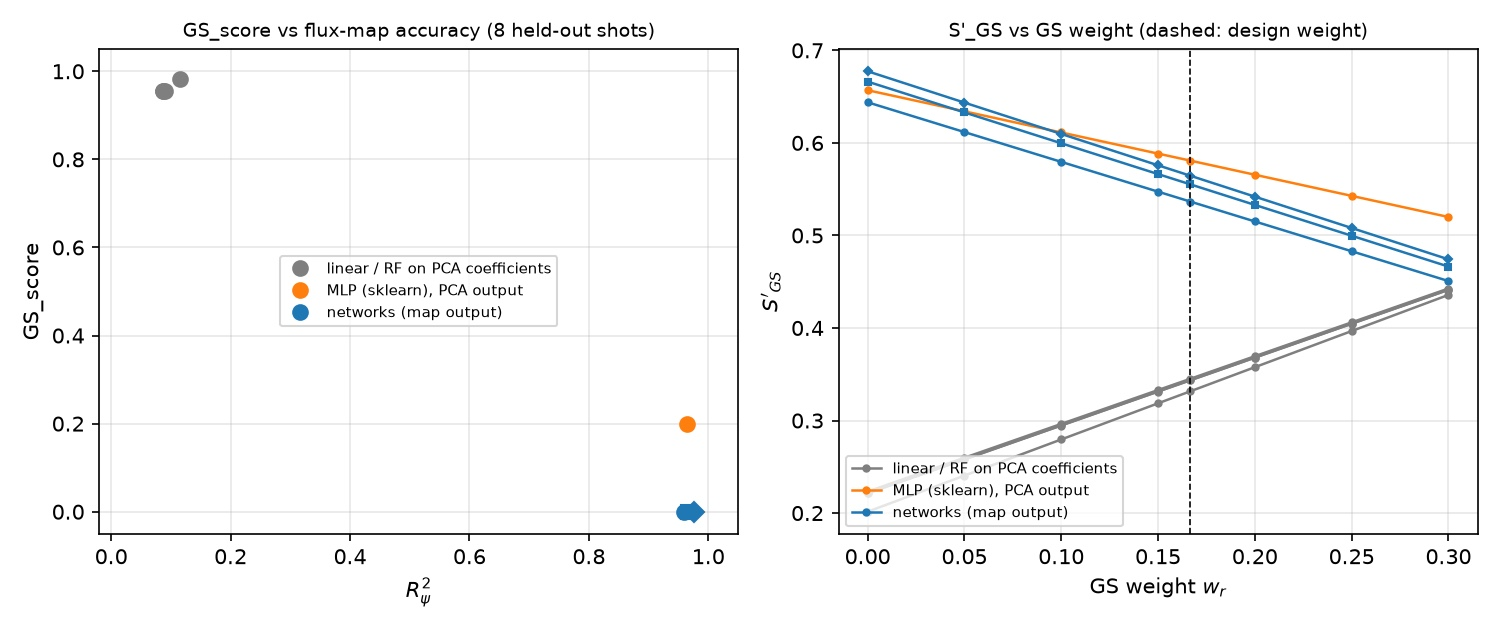
\includegraphics[width=\textwidth]{g04_c4_gs.jpg}
\caption{Ліворуч: $\mathrm{GS}_{\mathrm{score}}$ проти $R^2_\psi$ для восьми моделей. Праворуч: $S'_{\mathrm{GS}}$ залежно
від ваги $w_r$ (пунктир --- головна вага). Власний розрахунок, код: \texttt{Our try/04-novelty/c4/\{evaluate,summarise\}.py}.}
\label{fig:g04-c4}
\end{figure}

За $S'_{\mathrm{GS}}$ MLP (sklearn) піднімається на перше місце ($\tau$ Кендалла $=0{,}857$), але
лише в 74--75\,\% повторень; навіть при $w_r=0{,}30$ --- 94\,\% і 84\,\%. Групи «лінійні» ($S\approx0{,}19$)
і «мережі» ($S\approx0{,}65$) розділені надто сильно, щоб член вагою до 0,30 їх переставив
(рис.~\ref{fig:g04-c4}, праворуч).

\begin{refuted}{R12 (половина гіпотези C4)}
«$\mathrm{GS}_{\mathrm{score}}$ змінить упорядкування бейзлайнів». Точковий порядок змінюється, але
жодна перестановка не тримається в 95\,\% повторень. Частина C4 про Calibration лишається відкритою
\cite{RegEst}.
\end{refuted}

\begin{established}{E38}
Карти потоку мереж із виходом-картою мають $R^2_\psi=0{,}96\text{--}0{,}98$, але $g=0{,}81\text{--}0{,}96$ ---
більше, ніж в істини з 1\,\% шуму: за рівнянням ГШ це взагалі не рівноваги. Моделі на коефіцієнтах
PCA мають $g=0{,}02\text{--}0{,}03$ завдяки гладкості, а не фізиці ($R^2_\psi\approx0{,}09$). Член
антикорелює з $R^2_\psi$ (Спірмен $-0{,}60$) \cite{RegEst}.
\end{established}

\paragraph{Що з цього випливає.} У теперішньому вигляді $\mathrm{GS}_{\mathrm{score}}$ --- не оцінка якості,
а \emph{шлюз}: він надійно відділяє «не рівновагу» від рівноваги, але нагороджує гладкість. Природніше
множити ($S\times$допуск) або ставити поріг на $g$, ніж додавати. Ризик, про який попереджала E8,
справдився.

\section{C6: калібрування невизначеності поля}\label{sec:g04-c6}

\begin{conjecture}{C6}
Одночасні конформні смуги на полі $65\times65$~--- правильна форма UQ-члена. \emph{Спростує:} емпіричне покриття виявиться недосяжним без абсурдної ширини смуг. \emph{Вартість:} близько дня~\cite{RegConj}.
\end{conjecture}

\begin{outofcorpus}[конформні передбачення]
Роздільне (split) конформне передбачення: на калібрувальній вибірці з $n$ кадрів рахуємо оцінки $s_i$. Для поля зручна max-статистика $s_i=\max_{x}|\hat\psi_i(x)-\psi_i(x)|/\hat\sigma(x)$. Беремо $\lceil(n+1)(1-\alpha)\rceil$-ту в порядку зростання оцінку $\hat s$. Смуга $\hat\psi(x)\pm\hat s\,\hat\sigma(x)$ покриває \emph{все поле одночасно} з імовірністю не менше $1-\alpha$, якщо дані обмінювані (exchangeability), причому без жодних припущень про розподіл і незалежно від якості базової моделі. Поточкові інтервали дали б 4\,225 окремих маргінальних гарантій замість однієї спільної.
\end{outofcorpus}

Отже, питання C6 справді математичне: який спосіб обрати~--- max-статистику, проєкцію на базис PCA чи конформізацію похідних скалярів замість пікселів (\texttt{metric-design.md}). Захист від геймінгу обов'язковий: нескінченно широка смуга має ідеальне покриття. Тому \eqref{eq:g04-calib} треба доповнити штрафом за ширину (нормування ширини, CRPS або логарифмічна передбачувальна щільність) \emph{до} публікації правил. Стан ніші за \texttt{our-contribution.md}: «підтверджено тонкою». GP-томографія дає UQ у замкненій формі, але відкидає баланс сил, а EFIT-Prime не доводить частотного калібрування.

\section{Побічна знахідка: функція Гріна з неправильним аргументом (E33)}\label{sec:g04-e33}

\begin{established}{E33 --- виправлено 2026-09-29}
У \texttt{Tokamak-GS-solver} функції \texttt{ellipk}/\texttt{ellipe} отримували модуль $k$ замість параметра $m=k^2$. Похибка старої $G$ сягала $+9\,\%$ біля нитки, $+42\,\%$ при $k^2=0{,}95$ ($3{,}355\cdot10^{-7}$ проти $2{,}355\cdot10^{-7}$ Вб/рад/А) і $\times8$ при $k^2=0{,}5$. Після виправлення відхилення від квадратури Біо--Савара становить $\sim10^{-15}$~\cite{RegEst,g04GSsolverChanges}.
\end{established}

\code{gs/src/numerical/compute.py}{12}{31}{(функція Гріна кругової нитки, після виправлення)}

Рядки 26--29: параметр $k^2$ обчислюється явно і передається в \texttt{special.ellipk}/\texttt{ellipe}, бо SciPy очікує саме $m=k^2$. Рядок 30 містить формулу $G=\frac{\mu_0}{2\pi}\frac{\sqrt{RR_0}}{k}\big[(2-k^2)K(k^2)-2E(k^2)\big]$. Чому помилка така велика далеко від нитки? За $k\to0$ дужка $(2-k^2)K-2E\propto k^4$ є результатом тонкого взаємного скорочення великих доданків. Якщо обчислити $K$ і $E$ у точці $k$ замість $k^2$, скорочення руйнується, і потік від далеких котушок помиляється на порядки (див.~\cite{g04GSsolverChanges}, §2). Це той самий урок, що й у \S\ref{sec:g04-physics}. Величини, отримані з \emph{різниць} великих чисел (скорочення в $G$, друга похідна в $\GSop$), підсилюють малі похибки входу. Тому для них потрібні незалежні перевірки: квадратура для $G$ (\texttt{tests/test\_green.py}) і нев'язка $g$ для $\psi$. Усі \texttt{result/PINN\_*.png}, зроблені до 29.09, використовували хибну $G$.

\begin{practicum}[C4 і C6: студентські задачі]
\textbf{Відтворити} (з теки \texttt{fusion equilibrium challenge/starter}, $\approx$20~с і $\approx$4~с):
\texttt{.venv/bin/python "../../Our try/04-novelty/gs\_residual\_probe.py"}; \texttt{.venv/bin/python ../../manual/code/ch11\_gs\_residual\_baseline.py}.

\textbf{Задача~1 (R12 $\to$ шлюз, пів дня).} Половину C4 спростовано (\S\ref{sec:g04-c4test}). Спробуйте $\mathrm{GS}_{\mathrm{score}}$ як шлюз: $S\cdot\mathbb 1[g<g_{\mathrm{ref}}]$ або м'якшу шкалу $\log g$. Чи з'являться стійкі перестановки, і чи вони розумні (лінійні моделі не мають вигравати лише завдяки гладкості)? Код і прогнози --- \texttt{Our try/04-novelty/c4/}.

\textbf{Задача~2 (самоперевірки).} Перевірте чисельно $g(-\psi)=g(\psi)$ (перевірка 4) і стійкість до порядку базису: $n_p,n_f=2\ldots8$ (перевірка 6). Як змінюється відношення $g(\text{шум }1\,\%)/g(\text{істина})$?

\textbf{Задача~3 (C6, день).} Розбийте кадри на навчальні й калібрувальні \emph{за розрядами}, а не за кадрами, інакше обмінюваність порушено. Побудуйте max-статистичну смугу для $\alpha=0{,}1$ і виміряйте емпіричне покриття та середню ширину на відкладених розрядах. Якщо покриття 90\,\% досягається лише зі смугою, ширшою за $\mathrm{std}(\psi)$, це аргумент на користь спростування C6.
\end{practicum}

\chapter{Топологія \texorpdfstring{$\psi$}{ψ}: O- і X-точки}\label{ch:g05}

GS-нев'язка з розд.~\ref{ch:g04} спрацьовує вже на 1\,\% шуму, але вона кількісна. Цей розділ про якісний, бінарний критерій: чи має подане поле взагалі \emph{топологію} рівноваги токамака? Тут розглянуто пункти E9--E13 (з уточненням N4, внесеним у реєстр 2026-09-29), спростування R5 і перевірку V-D4. Геометрію O- і X-точок див. у~\cite{Manual}, розд.~4.

\section{Фізика: критичні точки, індекс, Пуанкаре--Хопф, Морс}\label{sec:g05-physics}

Критична точка $\psi(R,Z)$~--- це точка, де $\grad\psi=0$, тобто полоїдальне поле $\Bpol=|\grad\psi|/R$ дорівнює нулю. Тип точки визначає гесіан $\mathsf H_\psi$. Якщо $\det\mathsf H_\psi>0$, маємо екстремум: це \emph{O-точка} (еліптична). Навколо неї лежать вкладені магнітні поверхні. Магнітна вісь~--- саме така точка, і зайва O-точка означає магнітний острів. Якщо $\det\mathsf H_\psi<0$, маємо сідло: це \emph{X-точка} (гіперболічна), через яку проходить сепаратриса.

\paragraph{Індекс (winding number).} Обійдемо малий контур навколо ізольованої критичної точки і порахуємо, скільки обертів робить вектор $\grad\psi$. Для екстремуму індекс дорівнює $+1$, причому \emph{однаково} для максимуму й мінімуму (при $\psi\to-\psi$ вектор просто повертається на $\pi$). Для сідла індекс $-1$. Саме тому критерій не залежить від знакової конвенції машини, що знадобиться в розд.~\ref{ch:g06}.

\begin{outofcorpus}[теорема Пуанкаре--Хопфа і теорія Морса]
\emph{Пуанкаре--Хопф.} Нехай поле $\grad\psi$ на межі області $D$ всюди напрямлене назовні (або всюди всередину) і має скінченну кількість нулів. Тоді сума індексів нулів у $D$ дорівнює ейлеровій характеристиці $\chi_{\mathrm E}(D)$. Для диска $\chi_{\mathrm E}=1$, тож усередині замкненої магнітної поверхні $N_O-N_X=1$.

\emph{Морс.} Для функції Морса ейлерова характеристика підрівневої множини $\{\psi\le t\}$ змінюється лише тоді, коли $t$ проходить критичне значення: на $+1$ при мінімумі чи максимумі (індекс Морса 0 чи 2) і на $-1$ при сідлі (індекс Морса 1). Отже,
\begin{equation}\label{eq:g05-morse}
  \chi_{\mathrm E}\big(\{\psi\le t\}\cap D\big)=\sum_{c:\ \psi(c)\le t}(-1)^{\lambda_c}.
\end{equation}
Тобто $\chi_{\mathrm E}$-крива~--- це \emph{інтеграл} (кумулятивна сума) лічильника критичних точок зі знаком.
\end{outofcorpus}

Звідси три наслідки, які нижче перевірено числами.
\begin{enumerate}
\item У справжній рівновазі всередині LCFS маємо рівно одну O-точку і жодного сідла, сума індексів $+1$ (E9).
\item Шум народжує критичні точки \emph{парами}: у складці (saddle-node) з'являються екстремум і сідло разом. Кількість зростає, а сума індексів $+1-1=0$ не змінюється. Отже, сума як метрика марна, інформацію несе лише кількість (E11).
\item Пара O--X, що народилася поруч, дає в \eqref{eq:g05-morse} внески $+1$ і $-1$, які майже одразу скорочуються. Тому $\chi_{\mathrm E}$-крива менш чутлива за лічильник (E13, R5).
\end{enumerate}

\section{Звідки ідея}\label{sec:g05-origin}

Ідея прийшла з аналізу перерізу Пуанкаре (розд.~\ref{ch:g07}). В осесиметрії система силових ліній інтегровна, і переріз дає рівно контури $\psi$ (E18). Тому динамічний зміст, що лишається у 2D,~--- це не сам переріз, а \emph{скелет критичних точок} $\psi$. Так мотивовано docstring \texttt{topology\_probe.py}.

\emph{Увага:} до 2026-09-29 у рядках 6--7 цього docstring стояло «psi as canonical momentum»~--- та сама помилка, що R4 (правильно: імпульс~--- $\psit$, гамільтоніан~--- $\psi$, розд.~\ref{ch:g07}). На код вона не впливала; docstring виправлено 2026-09-29 без зміни кількості рядків~\cite{RegLog}.

Новизну перевірено в журналі (V-D2~\cite{RegVerif}): метод опубліковано в сегментації (Clough та ін., топологічна втрата без міток, лише з апріорної топології) і в стисненні даних (cpSZ). Нове лише \emph{застосування}: ніхто не робить кількість зайвих критичних точок метрикою фузійних сурогатів, і жоден фузійний бенчмарк не має топологічного члена.

\section{Де це в коді}\label{sec:g05-code}

\code{ourtry/04-novelty/topology_probe.py}{39}{48}{(індекс як число обертів $\grad\psi$)}

Рядки 41--44 обходять периметр прямокутника $[i_{z0},i_{z1}]\times[i_{r0},i_{r1}]$ проти годинникової стрілки. Рядок 45 бере кут $\arg\grad\psi$ у кожній точці периметра. Рядки 46--47 рахують прирости кута, зведені до $(-\pi,\pi]$, і це ключовий крок: без зведення стрибок $2\pi$ на розрізі $\arctan$ зіпсував би суму. Рядок 48 дає повне число обертів~--- індекс.

\code{ourtry/04-novelty/topology_probe.py}{51}{79}{(\texttt{critical\_points}: попіксельне детектування)}
\code{ourtry/04-novelty/topology_probe.py}{80}{90}{(продовження: зв'язні компоненти)}

\begin{itemize}
\item \textbf{Рядки 64--66}: $\grad\psi$ через \texttt{np.gradient} і кут \texttt{arctan2}.
\item \textbf{Рядки 69--78}: для кожного пікселя всередині області~--- число обертів по кільцю з восьми сусідів (\texttt{LOOP}, рядок 36). Ненульове значення означає, що в комірці сидить критична точка.
\item \textbf{Рядки 80--89}~--- \emph{виправлення V-D4}. Перша версія детектора рахувала попіксельні детекції як окремі точки і на істині давала \textbf{4 точки замість 1}. Діагностика показала кластер $2\times2$ навколо \emph{тієї самої} магнітної осі: вісь ($R=1{,}678$, $Z=+0{,}030$) лежить між пікселями, тож кільця чотирьох сусідніх пікселів усі її охоплюють~\cite{RegVerif}. Виправлення: детекції об'єднуються у зв'язні компоненти (\texttt{scipy.ndimage.label} зі зв'язністю 8), і для кожної компоненти рахується число обертів по периметру її обмежувального прямокутника, розширеного на одну комірку. Це математично коректний індекс усього, що лежить усередині.
\end{itemize}

\code{ourtry/04-novelty/topology_probe.py}{93}{102}{(область аналізу)}

Область~--- внутрішність LCFS, видобутої процедурою скорера, з ерозією на дві комірки (рядок 102). Ерозія тут не косметика. Вона виключає X-точку, що лежить \emph{на} сепаратрисі, і відсуває межу області всередину, де $\grad\psi\neq0$ і (для гладкого $\psi$) трансверсальний до межі~--- саме цього вимагає Пуанкаре--Хопф. Строго для піксельної області й зашумленого поля це не доведено, лише правдоподібно (коментар путівника). Журнал V-D4 окремо наголошує: сума $+1$ виходить \emph{тому}, що X-точки виключено. На прямокутнику, що містить $k$ X-точок, сума дорівнює $1-k$, і в конфігурації double-null критерій без явно зафіксованої області ламається.

\section{Що вийшло: E9--E11}\label{sec:g05-results}

\begin{established}{E9, E10, E11}
\textbf{E9.} Скелет істини точно канонічний: рівно 1 еліптична точка, 0 сідел, сума індексів $+1$.
\textbf{E10.} Скелет стійкий до 3\,\% шуму і руйнується на 10\,\%: при $R^2_\psi=0{,}993$ маємо 20,5 зайвих нерухомих точок.
\textbf{E11.} Сума індексів зберігається навіть у хаосі. Пуанкаре--Хопф змушує точки народжуватися парами O--X, тож як метрика сума марна, працює лише кількість~\cite{RegEst}.
\end{established}

Повторний запуск 2026-09-29 (\texttt{topology\_probe.py}, 8 кадрів розряду 203702, зерна $1000+k$) відтворив E9--E11. До рівня шуму 3\,\% включно медіани дорівнюють 1~O, 0~X, сума $1{,}0$ і 0 зайвих. На 10\,\% ($R^2_\psi=0{,}99278$) маємо 10,5~O, 11,0~X, медіану суми 1,5 і 20,5 зайвих. Рис.~\ref{fig:g05-cp} показує один кадр.

\begin{figure}[htbp]\centering
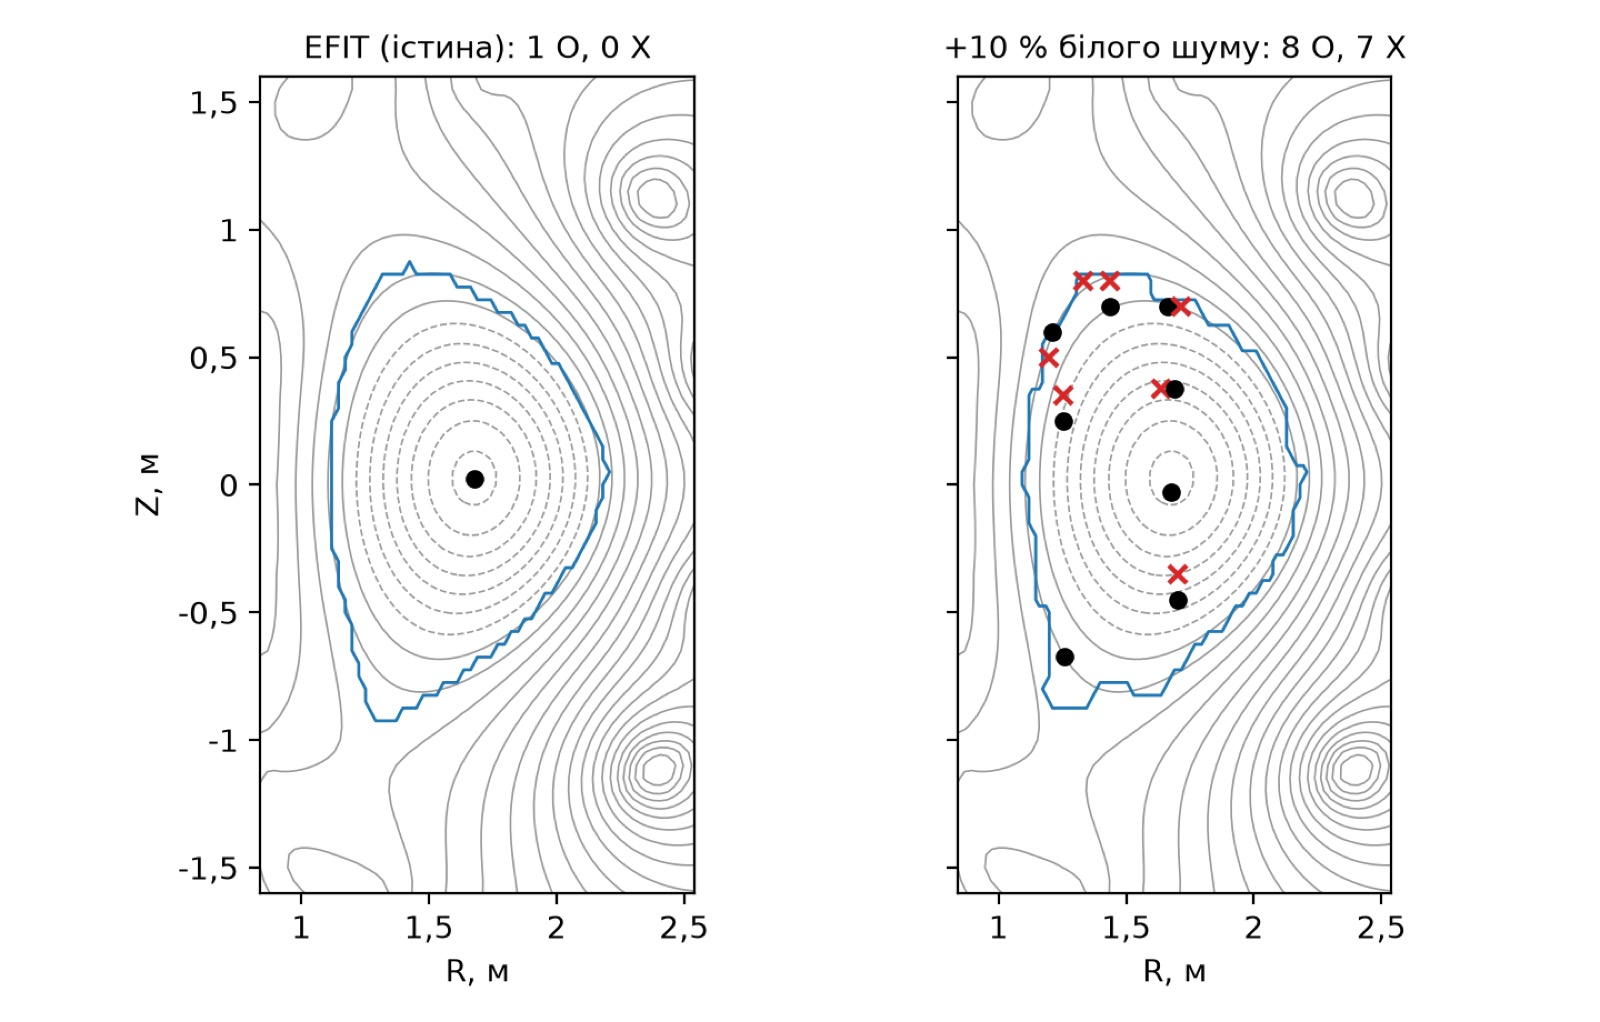
\includegraphics[width=0.8\textwidth]{g05_critical_points.jpg}
\caption[Критичні точки psi: істина і 10 \% шуму]{Критичні точки $\psi$ усередині LCFS (синій контур~--- область після ерозії) для кадру 75 розряду DIII-D 203702. Ліворуч: EFIT, рівно одна O-точка (магнітна вісь). Праворуч: +10\,\% білого шуму, 8~O ($\bullet$) і 7~X ($\times$), сума індексів $+1$. Сірим показано контури істинного $\psi$. Власний розрахунок функціями \texttt{inside\_lcfs}, \texttt{critical\_points} з \texttt{topology\_probe.py}; рисунок~--- \texttt{guide/figures/g05\_fig.py}. Дані: Fusion Equilibrium Challenge (Sophelio / General Atomics), CC BY 4.0.}\label{fig:g05-cp}
\end{figure}

\paragraph{Уточнення N4 (внесено в реєстр 2026-09-29).} Поріг 3\,\% \emph{пограничний}. \texttt{topology\_probe.py} на 3\,\% дає медіану 1~O/0~X, тобто лічильник мовчить. Натомість \texttt{topology\_ec\_curve.py} на іншій реалізації шуму (зерна $7000+k$, 6 кадрів) дає медіану лічильника 1,5, тобто лічильник спрацьовує. Обидва скрипти перезапущено, числа відтворились. Тому «стійкий до 3\,\%» слід читати як «на межі стійкості». Для E11 медіана суми при 10\,\% дорівнює 1,5, тобто «близька до $+1$», а не рівна $+1$. Висновок «сума марна, працює кількість» від цього не змінюється~\cite{RegEst}. Одне спостереження з нашого прогону: на 10\,\% другий скрипт дає медіану 17,0 критичних точок, тобто 16 зайвих, проти 20,5 у першого. Масштаб той самий, але точне число залежить від реалізації шуму й набору кадрів.

\section{Ейлерова характеристика: еталон без налаштування (E12) і спростування R5}\label{sec:g05-ec}

\code{ourtry/04-novelty/topology_ec_curve.py}{25}{32}{($\chi_{\mathrm E}$-крива підрівневих множин)}

Для кожного з 40 порогів $t$ маска $\{\psi\le t\}\cap D$ передається в \texttt{skimage.measure.euler\_number} зі зв'язністю 1. Складність $\order{N}$ на рівень. На DIII-D вісь є \emph{мінімумом} $\psi$ (\texttt{AXIS\_SIGN}$=-1$, розд.~\ref{ch:g06}), тож $\{\psi\le t\}$ поблизу осі~--- диск.

\code{ourtry/04-novelty/topology_ec_curve.py}{59}{85}{(порівняння на одній драбині шуму)}

Рядки 66--69: $\chi_{\mathrm E}$-криву збуреного поля рахують на \emph{еталонній} масці й еталонних порогах, щоб метрику не збивало зміщення передбаченої LCFS. Рядки 70--74 обчислюють середнє і максимальне $|\Delta\chi_{\mathrm E}|$ та кількість критичних точок тим самим детектором. Рядки 77--84 формулюють вердикт: «EC fires», якщо середнє $|\Delta\chi_{\mathrm E}|>1$; «count fires, EC quiet», якщо критичних точок більше однієї.

\begin{established}{E12, E13}
\textbf{E12.} На істині $\chi_{\mathrm E}(\psi\le t)\equiv1$ на всіх рівнях: кожна підрівнева множина є диском. Це еталон без налаштування, для якого не треба знати кількість O-точок і не потрібен поріг персистентності.
\textbf{E13.} $\chi_{\mathrm E}$-крива менш чутлива за лічильник: вона мовчить на 3\,\%, де лічильник спрацьовує. За Морсом вона є його інтегралом~\cite{RegEst}.
\end{established}

Прогін 2026-09-29: на 3\,\% ($R^2_\psi=0{,}99956$) середнє $|\Delta\chi_{\mathrm E}|$ дорівнює 0,138 при медіані лічильника 1,5 (вердикт «count fires, EC quiet»). На 10\,\% маємо 4,075, тобто спрацьовують обидва. На істині $\chi_{\mathrm E}=1$ у всіх надрукованих рівнях.

\begin{refuted}{R5}
«$\chi_{\mathrm E}$-крива краща за лічильник критичних точок». Це була наша власна рекомендація; журнал V-D4 фіксує, що вона хибна. Вимір показав протилежне: крива \emph{менш} чутлива, бо за \eqref{eq:g05-morse} вона є інтегральною версією лічильника, а не незалежним виміром~\cite{RegEst,RegVerif}. Вона не марна: $\chi_{\mathrm E}\equiv1$ зручно подавати як \emph{шлюз} (див. \texttt{metric-design.md}, розділ «Шлюз»). Діагностику ж, тобто скільки зайвих островів і де саме, дає лічильник.
\end{refuted}

Чутливість топологічного критерію нижча за GS-нев'язку: 3\,\% проти 1\,\% шуму. Звідси його роль у \texttt{metric-design.md}: не градуйований член, а \emph{критерій допустимості}, пізніший, але якісно інший сигнал. Він ловить острови, яких не існує.

\begin{practicum}[топологічний шлюз]
\textbf{Відтворити} (з \texttt{fusion equilibrium challenge/starter}, $\approx$40~с і $\approx$60~с): \texttt{.venv/bin/python "../../Our try/04-novelty/topology\_probe.py"} і \texttt{... topology\_ec\_curve.py}.

\textbf{Задача~1 (N4 кількісно).} Замініть одне зерно на кадр (рядок 126, \texttt{1000 + k}) циклом по 20 зернах і оцініть \emph{імовірність} того, що лічильник спрацює на 1, 2, 3 і 5\,\% шуму. Поріг стане кривою ймовірності замість «так/ні».

\textbf{Задача~2 (персистентність).} \texttt{metric-design.md} вимагає персистентного порогу замість склеювання компонент, інакше детектор галюцинує точки в SOL. Відкидайте пари O--X, для яких $|\psi_O-\psi_X|$ менший за поріг $\tau$. За якого $\tau$ істина лишається $1/0$, а 10\,\% шуму ще ловиться?

\textbf{Задача~3 (double-null).} Візьміть прямокутник, що містить X-точку, без ерозії LCFS і переконайтеся, що сума індексів дорівнює $1-k$. Запропонуйте явне означення області для конфігурації з двома X-точками.
\end{practicum}

\chapter{Перенесення між машинами}\label{ch:g06}

Цей розділ~--- історія гіпотези, яку спростували з користю. Гіпотеза H5 припускала, що провал перенесення DIII-D$\to$MAST має топологічну складову. Вимір показав протилежне (R7), а звідси вийшли два встановлені факти: критерій машинно-незалежний (E15), і топологія переживає перенесення там, де значення не переживають (E16). Нижче також розглянуто колишню гіпотезу C8 (2026-09-29 спростовано як артефакт знака~--- R9), відкладені C9 і C10, ліцензійне питання Q13 і ліцензії E28.

\section{Звідки H5}\label{sec:g06-h5}

Наївне перенесення між машинами в пілоті челенджу падає з SSIM 0,83 до 0,10 (\texttt{01-landscape/\allowbreak saturated-vs-\allowbreak headroom.md}, позначка [V]~\cite{g06Headroom}). Зазвичай це читають так: «значення не переносяться». H5 ставила гостріше питання (docstring \texttt{h5\_transfer\_topology.py}):

\begin{quote}\itshape
чи гірша топологія міжмашинного передбачення за топологію внутрішньомашинного передбачення тієї самої $L^2$-точності?
\end{quote}

Якби так, модель переносила б \emph{значення}, але не \emph{скелет}, і топологічний член розд.~\ref{ch:g05} побачив би відмову, яку $R^2$ сам по собі недооцінює.

\paragraph{Модель замість моделі.} Лінійний декодер, навчений на DIII-D, може видати лише поле з лінійної оболонки PCA-базису DIII-D. Тож проєкція \emph{істинного} MAST на цей базис дає \emph{верхню межу} того, що будь-який такий декодер міг би вивести для MAST, причому за ідеального знання цілі. Якщо навіть ця проєкція втрачає топологію, жодна така модель її не збереже. Контроль~--- проєкція DIII-D на власний базис того самого розміру.

\section{Конвенції знака: \texttt{AXIS\_SIGN}}\label{sec:g06-sign}

\code{fec/starter/fusion_scoring/common.py}{74}{89}{(знакові конвенції скорера FEC)}

Рядки 74--80: на DIII-D магнітна вісь лежить у \emph{мінімумі} збереженого $\psi$ (99,98\,\% з 1\,559\,340 кадрів), а в EFIT++/FAIR-MAST~--- у \emph{максимумі} (100\,\% кадрів MAST). Тому \texttt{AXIS\_SIGN}$=\{-1,+1\}$, і скорер скрізь працює з добутком $\texttt{AXIS\_SIGN}\cdot\psi$, у якому вісь завжди є максимумом. Коментар підкреслює, що машини мають \emph{однаковий} напрям струму: різниця походить від двох реалізацій EFIT, а не від фізики. Рядки 82--89: геометрично ідеальне передбачення для MAST у конвенції DIII-D давало б $R^2_\psi=-5{,}71$, гірше за сталу. Тому з версії v3.1 скорер інваріантний до знака. Він обирає \emph{один біт на машину на весь фолд}, тож знаком не можна «фармити» шум.

У топології знак нічого не змінює: і максимум, і мінімум мають індекс $+1$ (розд.~\ref{ch:g05}). Тому критерій повинен працювати на обох машинах без жодної поправки. Саме це перевіряє перший блок скрипта.

\section{Де це в коді}\label{sec:g06-code}

\code{ourtry/04-novelty/h5_transfer_topology.py}{61}{84}{(\texttt{skeleton}: область і попіксельні індекси)}
\code{ourtry/04-novelty/h5_transfer_topology.py}{85}{97}{(продовження: компоненти, O/X, сума)}

Це самодостатня копія детектора з \texttt{topology\_probe.py} (розд.~\ref{ch:g05}), параметризована машиною. Рядок 64 викликає \texttt{extract\_lcfs} з назвою машини, тобто з її \texttt{AXIS\_SIGN}. Якщо LCFS не знайдено, функція повертає \texttt{None} (рядки 65--66): це «провал вилучення», який з'явиться в C8. Рядки 69--72 будують область з ерозією на дві комірки і відкидають області менші за 40 пікселів. Рядки 73--84 рахують попіксельне число обертів, рядки 85--97~--- зв'язні компоненти (виправлення V-D4) і лічильники $N_O$, $N_X$ та суму індексів.

\code{ourtry/04-novelty/h5_transfer_topology.py}{128}{138}{(\texttt{project}: найкращий вихід DIII-D-декодера)}

Рядок 134: $\mathrm{rec}=\mu+(Y_s-\mu)V_k^{\mathsf T}V_k$~--- ортогональна проєкція на перші $k$ головних компонент DIII-D навколо середнього поля DIII-D $\mu$. Рядки 132--137 для MAST пробують обидва глобальні знаки $s=\pm1$ і лишають той, що дає меншу $L^2$-похибку, як і скорер. Для DIII-D (контроль) знак не шукається.

\code{ourtry/04-novelty/h5_transfer_topology.py}{147}{167}{(головний цикл по розміру базису; лічильник \texttt{nfail})}

Для $k=5,10,20,50$ рядки 148--155 обчислюють $R^2_\psi$ і медіанний скелет контролю на 8 кадрах. Рядки 157--162 роблять те саме для MAST, де $R^2$ рахується відносно \emph{знакоскоригованої} цілі $s_M\psi_M$. Рядок 160 рахує \texttt{nfail}~--- кількість кадрів, на яких \texttt{skeleton} повернув \texttt{None}. Рядки 164--166 друкують рядок таблиці з приміткою «[$n$/8 LCFS extraction failed]».

\section{Що вийшло: E15, E16, R7}\label{sec:g06-results}

Повторний запуск 2026-09-29 (3 демо-розряди на машину, 500 кадрів DIII-D і 115 кадрів MAST) відтворив таблицю:

\begin{center}\small
\begin{tabular}{r|cc|ccc}
\toprule
$k$ & $R^2_\psi$ D3D$\to$D3D & скелет & $R^2_\psi$ MAST$\to$D3D & скелет & знак $s_M$\\
\midrule
5  & 0,99987 & 1O/0X & 0,66248 & 1O/0X [3/8 провалів LCFS] & $-1$\\
10 & 1,00000 & 1O/0X & 0,87883 & 1O/0X & $+1$\\
20 & 1,00000 & 1O/0X & 0,92690 & 1O/0X [2/8 провалів LCFS] & $-1$\\
50 & 1,00000 & 1O/0X & 0,96298 & 1O/0X & $+1$\\
\bottomrule
\end{tabular}
\end{center}

\noindent На істині обидві машини мають 1 еліптичну точку, 0 гіперболічних і суму $+1$ на 8/8 кадрах.

\begin{established}{E15, E16}
\textbf{E15.} Топологічний критерій машинно-незалежний: DIII-D і MAST дають 1O/0X і суму $+1$, попри протилежні конвенції знака, різні сітки й різну геометрію.
\textbf{E16.} Топологія переживає перенесення там, де значення не переживають: у проєкції MAST на базис DIII-D $R^2_\psi$ падає до 0,66, а скелет лишається 1O/0X~\cite{RegEst}. (Примітку про рядок $k=50$ зареєстровано 2026-09-29, див. нижче.)
\end{established}

\begin{refuted}{R7 (H5)}
«Провал перенесення має топологічну складову». Топологія вціліла: при $R^2_\psi=0{,}66$ скелет 1O/0X. Інверсія виявилася кориснішою за саму гіпотезу, бо дала E15 і E16~\cite{RegEst}. У підсумку реєстру гіпотез R7 названо одним із двох спростувань, що дали «кращі результати після спростування», ніж містили до нього~\cite{RegConj}.
\end{refuted}

\begin{derivation}[чому гладка похибка не народжує критичних точок (оцінка путівника)]
Нова критична точка з'являється там, де похибка компенсує градієнт: $\grad\delta\psi=-\grad\psi$. Проєкція на кілька головних компонент дає \emph{гладку} похибку з малими $|\grad\delta\psi|$. Скрізь, крім малого околу осі, $|\grad\psi|$ більший, тож нових нулів немає. Поблизу осі невироджений екстремум (функція Морса) структурно стійкий щодо $C^1$-малих збурень: він лише зсувається, але не розщеплюється. Отже, топологію захищає мала похибка \emph{в $C^1$}, а не в $L^2$. Білий шум на сітці з кроком $h$ має $|\grad\delta\psi|\sim\varepsilon/h$ і тому народжує пари O--X (розд.~\ref{ch:g05}). Проєкція ж міжмашинна, велика в $L^2$, але гладка. Саме тому E16 не суперечить E10.
\end{derivation}

\paragraph{Застереження, знайдене при підготовці путівника.} Скрипт друкує \emph{медіани} по 8 кадрах з форматом \texttt{.0f}, а Python округлює 0,5 до парного, тобто до 0. Покадровий прогін (\texttt{guide/figures/g06\_h5\_frames.py}) для $k=50$ (MAST$\to$D3D) дав такі скелети: $(1,0,{+1})$ на чотирьох кадрах, $(1,1,0)$ на трьох і $(2,1,{+1})$ на одному. Отже, медіана $N_X=0{,}5$, а на половині кадрів в області є X-точка, хоча в таблиці стоїть «1O/0X». Для $k=10$ і для всіх контрольних рядків DIII-D усі кадри мають $(1,0,{+1})$; для $k=5$ усі 5 вилучених кадрів мають $(1,0,{+1})$, а для $k=20$ (6/8 вилучено) один кадр має $(1,1,0)$, медіана 0 (покадровий прогін \texttt{Our try/04-novelty/h5\_frames\_check.py}, 2026-09-29). E16 (твердження про $k=5$) це не зачіпає. Проте рядок $k=50$ показує, що топологічні дефекти при перенесенні \emph{можливі}, і H5 варто перевірити ще раз при \emph{порівнянному} $R^2_\psi$ (див. практикум). Зареєстровано 2026-09-29 як примітку до E16 (і посилання в R7); скрипт~--- \texttt{Our try/04-novelty/h5\_frames\_check.py}~\cite{RegEst,RegLog}.

\section{C8: провали вилучення LCFS}\label{sec:g06-c8}

\begin{conjecture}{C8 --- \emph{закрито 2026-09-29: спростовано як артефакт, тепер R9}}
\emph{Нижче~--- формулювання, яке діяло до 2026-09-29.} Провали вилучення LCFS на 3/8 і 2/8 кадрах MAST при перенесенні (E16)~--- \emph{систематичний сигнал}, а не шум. \emph{Спростує (переписано 2026-09-29):} на вибірці MAST з EFIT-рівновагами з FAIR-MAST (CC BY-SA 4.0) або іншого джерела, значно більшій за 3 демо-розряди, провали розподілені по $k$ випадково. \emph{Вартість:} $\approx2$~год обчислень \emph{плюс} невідома вартість отримання даних і ліцензійне обтяження BY-SA (Q13, V-C4). У нинішньому формулюванні гіпотеза нездійсненна: \texttt{efit\_psirz} для MAST на HF публікується лише для 3 демо-розрядів (N3)~\cite{RegConj}.
\end{conjecture}

\paragraph{Спостереження для путівника: провали збігаються зі знаком.} У таблиці вище провали є \emph{лише} в рядках, де пошук знака обрав $s_M=-1$ ($k=5$ і $k=20$). Ми перевірили це прямо тими самими функціями \texttt{load}, \texttt{skeleton} і тим самим базисом (\texttt{guide/figures/g06\_c8\_sign\_check.py}). Для кожного $k$ і обох знаків реконструкцію повертали в конвенцію MAST множенням на $s_M$, а потім шукали LCFS. Результат: зі знаком $+1$ провалів 0 для всіх $k$. Зі знаком $-1$ «як є» маємо 3, 2, 2 і 8 провалів з 8 (для $k=5,10,20,50$). Після повернення знака провалів 0 скрізь.

Механізм описано в docstring \texttt{extract\_lcfs\_with\_sign} скорера. Без явного \texttt{axis\_sign} функція спершу пробує конвенцію машини, а протилежний знак бере як запасний варіант за правилом «перший успіх, а не найкраще припасування». На інвертованій карті такий шлях дає хибні межі або провали. \texttt{skeleton} передає \texttt{"MAST"} без \texttt{axis\_sign}, тоді як реконструкція, обрана зі знаком $-1$, інвертована.

Отже, «систематичний сигнал» C8 виявився артефактом обробки знака в самому скрипті, а не властивістю перенесення; для перевірки вистачило 3 демо-розрядів, нових даних не знадобилося. Зареєстровано 2026-09-29 як \textbf{R9} (C8~→ спростовано, артефакт); скрипт~--- \texttt{Our try/04-novelty/c8\_sign\_check.py}~\cite{RegEst,RegConj,RegLog}. Сам \texttt{skeleton} не змінювали: передавати \texttt{axis\_sign} лишається задачею практикуму.

\section{Відкладені гіпотези і ліцензії}\label{sec:g06-deferred}

\begin{itemcard}{C9}{відкладено свідомо}
Перенесення між машинами можна покращити фізично коваріантним поданням: коефіцієнтами функцій Гріна замість пікселів (пор.~з архітектурою~\cite{McClenaghan2024}). Відкладено, бо це задача \emph{живого} змагання Sophelio. Беремо її як мотивацію, а не як власну роботу~\cite{RegConj}.
\end{itemcard}

\begin{itemcard}{C10}{відкладено свідомо}
Контамінація міток: частина похибки будь-якої ML-моделі~--- це успадковане зміщення EFIT, а не похибка моделі. Для перевірки потрібна незалежна істина, якої немає. Записано як відкрите питання поля~\cite{RegConj}. Зв'язок із цим розділом: DIII-D і MAST реконструйовані \emph{різними} реалізаціями EFIT (\texttt{AXIS\_SIGN}), тож частина «міжмашинної» різниці може бути різницею реконструкцій.
\end{itemcard}

\begin{established}{E28 (прочитано)}
Ліцензії: HDB5~--- CC BY 4.0; ConStellaration~--- MIT; дані Sophelio~--- CC BY 4.0; FAIR-MAST~--- CC BY-SA 4.0, причому share-alike поширюється на похідні бази через §4(b)~\cite{RegEst,RegVerif}.
\end{established}

\begin{itemcard}{Q13}{відкрите, блокує перевипуск частини MAST}
Яка правова підстава переходу 1\,206 розрядів MAST із CC BY-SA 4.0 (FAIR-MAST) у випуск CC BY 4.0 (Sophelio)? Share-alike поширюється на похідні бази через §4(b), тож перевипуск як простий CC BY сама BY-SA не дозволяє. Адресат~--- Sophelio та/або UKAEA. До з'ясування частину MAST трактуємо як обтяжену BY-SA; частину DIII-D це не зачіпає~\cite{RegQ,RegVerif}. Переписана 2026-09-29 версія C8 потребувала саме даних FAIR-MAST і впиралася в це питання; після закриття C8 як R9 нові дані для неї не потрібні.
\end{itemcard}

\begin{practicum}[перенесення і топологія]
\textbf{Відтворити} (з \texttt{fusion equilibrium challenge/starter}, $\approx$1--2~хв): \texttt{.venv/bin/python "../../Our try/04-novelty/h5\_transfer\_topology.py"}.

\textbf{Задача~1 (C8 без нових даних).} У \texttt{skeleton} передайте в \texttt{extract\_lcfs} явний \texttt{axis\_sign=s\_M*AXIS\_SIGN["MAST"]} (сигнатуру доведеться розширити). Чи зникнуть провали? (Відповідь для перевірки: так, 0 провалів при всіх $k$~--- R9.)

\textbf{Задача~2 (H5 чесно).} Замість медіан друкуйте покадрові трійки $(N_O,N_X,\Sigma)$. Потім зрівняйте $R^2_\psi$: для контролю DIII-D додайте шум або зменште $k$ до 1--3, щоб отримати $R^2\approx0{,}96$, і порівняйте частку кадрів з внутрішньою X-точкою з рядком MAST при $k=50$. Чи з'являється топологічна складова H5 при порівнянній точності?

\textbf{Задача~3 (знак).} Поясніть, чому оптимальний $s_M$ стрибає між $-1$ і $+1$ зі зміною $k$ (різниця похибок при $k=10$: 114 проти 126). Чим це відрізняється від правила скорера «один біт на фолд»?
\end{practicum}

\chapter{Переріз Пуанкаре й обернена задача}\label{ch:g07}

Це найдовша історія в проєкті. Спершу ми двічі помилилися в канонічних змінних (V-D3, R4) і з'ясували, що симплектична нейромережа~--- не наша ідея (V-D1, R3). Потім пілот D3 показав, що одномодова обернена задача тривіальна, а наше багатомодове узагальнення зламане (R8). Потім стенд \texttt{tokamak-3d-viz} зняв блокер і з'ясував, що в лінеаризованій постановці складність задачі задає не фізика, а вибір спостережуваного (VE21--VE25, VE30, VE31). Нарешті 2026-10-01 нелінійна перевірка за критеріями, записаними до запуску, закрила гіпотезу C5: базовий фіт не дійшов до рівня шуму на жодному стенді (R13), бо ландшафт нев'язки «скляний» (E40). Гамільтонів опис силових ліній і острови див. у~\cite{Manual}, розд.~2.

\section{Фізика: силова лінія як гамільтонова система}\label{sec:g07-ham}

У магнітних координатах $(\psit,\thetastar,\tor)$ поле токамака (з точністю до знака конвенції) має вигляд
\begin{equation}\label{eq:g07-B}
  \Bvec=\grad\psit\times\grad\thetastar+\grad\tor\times\grad\psi ,
\end{equation}
де $\psit$~--- тороїдальний потік на радіан, а $\psi$~--- полоїдальний. Уздовж силової лінії маємо
\begin{equation}\label{eq:g07-hamilton}
  \frac{\dd\thetastar}{\dd\tor}=\frac{\pa\psi}{\pa\psit}=\frac1q,\qquad
  \frac{\dd\psit}{\dd\tor}=-\frac{\pa\psi}{\pa\thetastar}.
\end{equation}
Це рівняння Гамільтона з півтора ступенями вільності: час~--- $\tor$, координата~--- $\thetastar$, імпульс~--- $\psit$, гамільтоніан $H=\psi$.

\begin{established}{E18--E20 (прочитано)}
\textbf{E18.} В осесиметрії $\psi=\psi(\psit)$ не залежить від $\thetastar$ і $\tor$. Тоді $\psit$ зберігається, система інтегровна, і переріз Пуанкаре дає \emph{рівно} контури $\psi$.
\textbf{E19.} Канонічний словник: час~--- $\tor$, координата~--- $\theta$, імпульс~--- \emph{тороїдальний} потік, гамільтоніан~--- \emph{полоїдальний}.
\textbf{E20.} Одна резонансна мода не дає хаосу: гамільтоніан $\psi_0(\psit)+A\cos(m\thetastar-n\tor)$ у гвинтовому куті $\xi=m\thetastar-n\tor$ не залежить від часу, тож система інтегровна~\cite{RegEst,Escande2024}.
\end{established}

\begin{established}{E39 (прочитано й перевірено, 2026-10-01)}
Обернене до E18 («немає осесиметрії~--- немає вкладених поверхонь») хибне. Landreman~\cite{Landreman2026} дав явні гладкі тороїдальні 3D-рівноваги МГД з $\grad p\ne0$ скрізь, крім осі, з вкладеними поверхнями і відхиленням від осесиметрії порядку одиниці: сімейство з $\iota\equiv2$ (усі лінії замкнені) і сімейство з широм. Ми перевірили статтю власним кодом: рівняння виконуються до $10^{-10}$--$10^{-12}$, числа $\beta_V=2/57$, $\iota(0)=2{,}28690$ відтворено, помилок не знайдено. \emph{Застереження, якого в статті немає:} у сімейства $\iota\equiv2$ саме поле $\Bvec$ має точну неперервну \emph{неізометричну} симетрію (еліптичне обертання, бо це лінійний образ поля Соловйова). Її порушують $|\Bvec|$, густина струму й тиск, тож як контрприклад до Ґреда це сімейство слабке. У сімейства зі широм афінної симетрії немає, але шир у прикладі статті лише $+0{,}04\,\%$~\cite{RegEst}. Код перевірки: \texttt{Our try/99-bibliography/landreman2026/}.  % lint-ok: E39 стосується неосесиметричних рівноваг, ι тут --- обертальне перетворення статті
\end{established}

\begin{refuted}{R4 (V-D3)}
«$\psi$ як канонічний імпульс». У нашому чернетковому формулюванні було саме так. Перевірка за~\cite{Escande2024} і Kallinikos та ін.~(2023; повних бібліоданих цієї праці в корпусі немає, лише згадка в реєстрі E19) виправила це до того, як помилка потрапила в матеріали хакатону~\cite{RegVerif}. Проте у вересні 2026 вона \emph{повторилася} в коді \texttt{tokamak-3d-viz}: ширину острова рахували з $\psi$ як імпульсом і завищували в $\sqrt q$ разів (N1, VR15). Виправлено 2026-09-29, деталі в розд.~\ref{ch:g08}. Ще один слід тієї самої помилки був у рядках 6--7 docstring \texttt{topology\_probe.py} (розд.~\ref{ch:g05}); його виправлено 2026-09-29.
\end{refuted}

\paragraph{Симплектичність.} Відображення Пуанкаре $(\psit,\thetastar)\mapsto(\psit',{\thetastar}')$ за один тороїдальний оберт є відображенням за час $2\pi$, породженим потоком гамільтонової системи. Тому воно зберігає площу (теорема Ліувілля): $\det\mathsf J=1$, де $\mathsf J$~--- якобіан відображення. Фізично це збереження магнітного потоку, $\grad\cdot\Bvec=0$. Мапа з $\det\mathsf J\ne1$ не є відображенням силових ліній, і все, що на ній виміряно, фізично нічого не означає.

\begin{refuted}{R3 (V-D1)}
«Симплектична нейромережа для відображень силових ліній~--- наша ідея». Спростовано: HénonNet~\cite{Burby2021} вчить відображення Пуанкаре силових ліній, і кожен його шар симплектичний за побудовою. Журнал верифікації додає ще одне: симплектичність є властивістю \emph{відображення}, а не статичного растра $\psi(R,Z)$. На осесиметричній сітці $65\times65$ вона вироджується в умову «$\psi$~--- добрий інваріант», тобто зводиться до GS-членів розд.~\ref{ch:g04}~\cite{RegVerif}.
\end{refuted}

\section{C5 і «Рівень 3»}\label{sec:g07-c5}

\begin{conjecture}{C5 (так її сформулювали; закрито 2026-10-01 $\to$ R13)}
Обернена задача Рівня~3 (спектр $(m,n)$) трактабельна за 48~год зі starter kit~\cite{RegConj}. Як гіпотезу перевірили й спростували~--- \S\ref{sec:g07-c5test}.
\end{conjecture}

\paragraph{Означення, додане ретроспективно 2026-09-29.} У корпусі «Рівень~3» вживався без означення, а Рівні~1--2 не визначені ніде. Реєстр гіпотез дає таке означення, прямо позначене як відновлене з контексту, а не цитоване~\cite{RegConj}:

\begin{quote}\itshape
Рівень~3~--- обернена задача на даних перетину Пуанкаре: за спостережуваною структурою силових ліній (проколи/екскурсії або слід на диверторі) відновити спектр збурення $(m,n)$, тобто амплітуди й фази мод.
\end{quote}

\noindent Про Рівні~1--2 нічого не стверджується.

\section{Пілот D3: Tokamap (E30)}\label{sec:g07-tokamap}

Перш ніж будувати інфраструктуру, пілот~\cite{g07D3} мав відповісти, чи обернена задача взагалі коректно поставлена. Стендом стала Tokamap~\cite{Balescu1998}: явне двовимірне відображення за один тороїдальний оберт, де $\Psi\ge0$~--- аналог тороїдального потоку (імпульс), а $T$~--- полоїдальний кут у частках $2\pi$.

\code{ourtry/03-deep-dives/D3-poincare-inverse/tokamap.py}{27}{54}{(профіль $q$, крок мапи, орбіта, $\det\mathsf J$)}

\begin{itemize}
\item \textbf{Рядки 27--28}: профіль $q(\Psi)=1+3\Psi^2$~--- \emph{наш} вибір, а не Балеску (docstring, рядки 14--16). Від нього залежить кожне кількісне число, але не якісна картина.
\item \textbf{Рядки 31--35} (\texttt{step}): $P=\Psi-1-\frac{x_L}{2\pi}\sin2\pi T$, $\Psi'=\tfrac12\big(P+\sqrt{P^2+4\Psi}\big)$, $T'=T+1/q(\Psi')-\frac{x_L}{4\pi^2}\frac{\cos2\pi T}{(1+\Psi')^2}\pmod 1$. Корінь квадратного рівняння гарантує $\Psi'\ge0$: вісь $\Psi=0$ мапа поважає автоматично, на відміну від стандартної мапи.
\item \textbf{Рядки 38--46} (\texttt{orbit}): ітерація з виходом при $\Psi<0$, $\Psi>20$ або нескінченності.
\item \textbf{Рядки 49--54} (\texttt{jacobian\_det}): $\det\mathsf J$ правими різницями з кроком $h=10^{-7}$. Похибка $\sim h$ задає «підлогу» $\sim10^{-8}$, нижче якої перевірка не бачить.
\end{itemize}

\begin{derivation}[чому Tokamap симплектична: твірна функція]
З рядка 33 випливає неявна форма $\Psi=\Psi'+\frac{x_L}{2\pi}\sin(2\pi T)\,f(\Psi')$, де $f(\Psi)=\Psi/(1+\Psi)$. Візьмемо твірну функцію другого роду
\[
  F(T,\Psi')=T\Psi'+G(\Psi')+h(T)\,f(\Psi'),\qquad G'=\frac1q,\qquad h(T)=-\frac{x_L}{4\pi^2}\cos2\pi T .
\]
Тоді $\Psi=\pa F/\pa T=\Psi'+h'(T)f(\Psi')$ і $T'=\pa F/\pa\Psi'=T+1/q(\Psi')+h(T)f'(\Psi')$, де $f'=(1+\Psi)^{-2}$. Це рівно рядки 32--34. Будь-яке відображення, породжене твірною функцією, симплектичне \emph{тотожно}. Нижче це знадобиться для R8.
\end{derivation}

\begin{established}{E30}
Tokamap реалізовано, і він точно симплектичний: $\max|\det\mathsf J-1|=5{,}6\cdot10^{-8}$ при $x_L=1{,}0$. $\Psi\ge0$ зберігається, перехід до хаосу монотонний~\cite{RegEst}.
\end{established}

Повторний запуск 2026-09-29 (\texttt{tokamap.py}) дав $\max|\det\mathsf J-1|$: $3{,}39\cdot10^{-9}$, $1{,}10\cdot10^{-8}$, $2{,}66\cdot10^{-8}$ і $5{,}64\cdot10^{-8}$ при $x_L=0$; 0,2; 0,5; 1,0. $\Psi\ge0$ виконується при $x_L=0{,}5$; 1,0; 2,0. Частка орбіт із розкидом $>0{,}3$ дорівнює 0 при $x_L\le0{,}5$, 0,083 при 0,8, 0,250 при 1,2 і 0,417 при 2,0 (рис.~\ref{fig:g07-tokamap}).

\begin{figure}[htbp]\centering
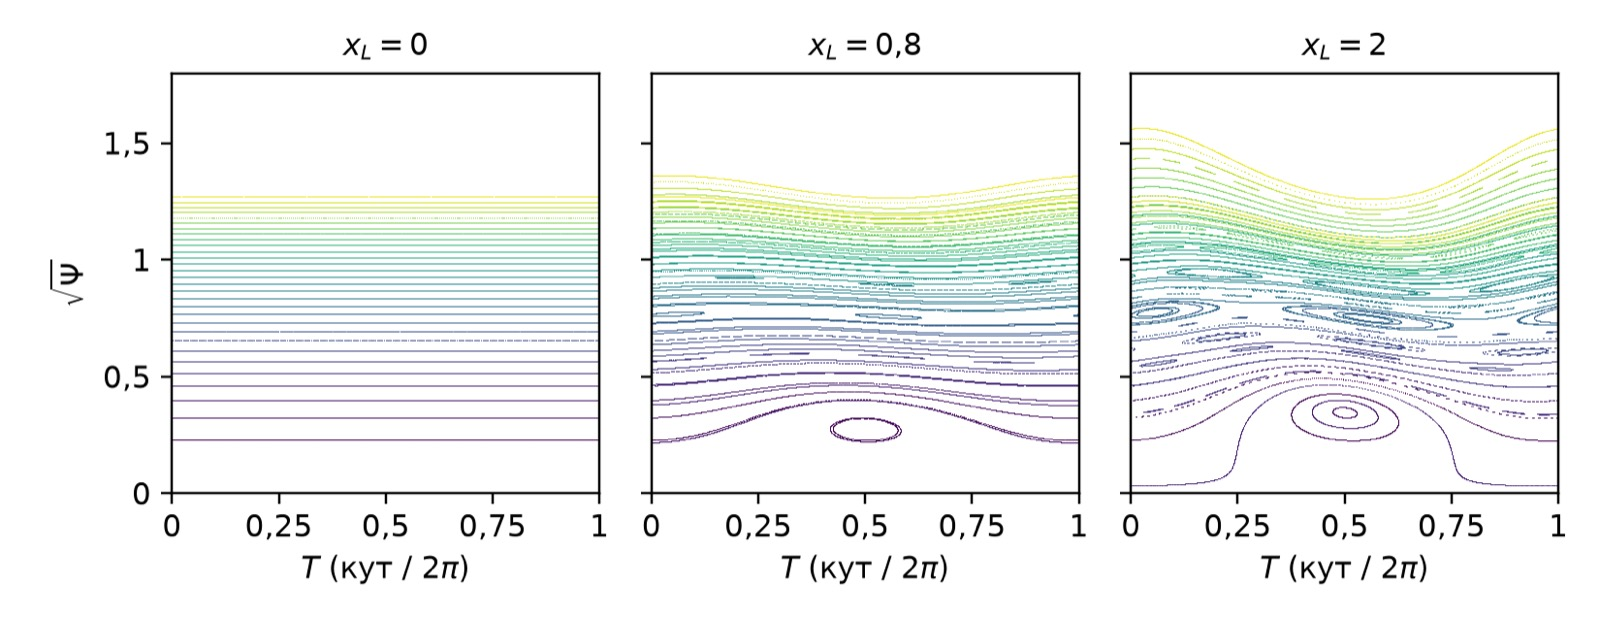
\includegraphics[width=\textwidth]{g07_tokamap.jpg}
\caption[Фазові портрети Tokamap]{Фазові портрети Tokamap ($q=1+3\Psi^2$) за 1\,500 ітерацій з 60 початкових умов. При $x_L=0$ маємо інваріантні кола (інтегровний випадок, аналог E18). Зі зростанням $x_L$ з'являються ланцюги островів на раціональних $q$ і розсіяні орбіти між ними. Власний розрахунок функцією \texttt{orbit} з \texttt{tokamap.py}; рисунок~--- \texttt{guide/figures/g07\_fig.py}.}\label{fig:g07-tokamap}
\end{figure}

\section{Пілот D3: спостережуване й ідентифіковність (E31, E32)}\label{sec:g07-ident}

\code{ourtry/03-deep-dives/D3-poincare-inverse/identifiability.py}{28}{46}{(усереднений профіль екскурсії)}

Спостережуване~--- радіальний профіль розкиду $\Psi$ за орбіту (\texttt{np.ptp} після 120 ітерацій прогріву), 32 радіуси. Ключовий рядок 34: для кожного радіуса беремо \texttt{N\_PHASE}$=24$ рівномірно розставлених початкових фаз $T_0$ зі спільним випадковим зсувом і усереднюємо. Перша версія брала \emph{одну} випадкову фазу.

\begin{established}{E31, E32}
\textbf{E31.} Спостережувана з однієї початкової фази непридатна: її шумова підлога 0,3244, а з усередненням по 24 фазах~--- 0,0006, у 540 разів краще. (Застереження: дві підлоги з різних стендів~--- зареєстровано 2026-09-29, див. нижче.)
\textbf{E32.} Відновити одну амплітуду тривіально: зміна $x_L$ на 3\,\% дає SNR 57, на 10\,\%~--- SNR 171. Для хакатону це не задача~\cite{RegEst}.
\end{established}

Повторний запуск: \texttt{identifiability.py} дає підлогу 0,0006 (максимум 0,0012), для +3\,\%~--- відносну зміну 0,0341 і SNR 56,6, для +10\,\%~--- 0,1028 і SNR 170,6. \texttt{multimode.py} відтворив підлогу 0,3244. \emph{Методичне застереження:} ці дві підлоги виміряно на \emph{різних} стендах. 0,3244 отримано на тримодовій мапі \texttt{multimode.py} ($a=0{,}3$, одна фаза), яка ще й не симплектична (R8), а 0,0006~--- на одномодовій Tokamap з $x_L=0{,}6$ і 24 фазами. Отже, «540$\times$» змішує ефект усереднення зі зміною стенда. Чистий ефект усереднення можна виміряти, поставивши \texttt{N\_PHASE}$=1$ в \texttt{identifiability.py} (практикум). Висновок E31, що одна фаза непридатна, це не скасовує: у \texttt{multimode.py} усі «сигнали» (0,38--0,43) лежать у межах шуму. Зареєстровано 2026-09-29 як застереження до E31: висновок про усереднення стоїть, відношення «540$\times$» кваліфіковано~\cite{RegEst,RegLog}.

\section{Пілот D3: зламане узагальнення (R8)}\label{sec:g07-r8}

\code{ourtry/03-deep-dives/D3-poincare-inverse/multimode.py}{30}{49}{(\emph{навмисно зламана} багатомодова мапа)}

Рядки 30--35: $V(T)=\sum_k\frac{a_k}{2\pi}\sin(2\pi m_kT+\varphi_k)$ і її похідна $V'(T)=\sum_ka_km_k\cos(\dots)$. Рядок 39 підставляє $V$ туди, де в Tokamap стоїть $\frac{x_L}{2\pi}\sin2\pi T$, а рядок 41 підставляє $V'/4\pi^2$ туди, де стоїть $\frac{x_L}{4\pi^2}\cos2\pi T$. Рядки 45--49 перевіряють $\det\mathsf J$ так само, як у \texttt{tokamap.py}. Симплектичність тут «перевіряється, а не припускається» (docstring), і перевірка її провалила.

\begin{refuted}{R8}
«Структуру Tokamap можна перенести на суму мод підстановкою $V'(T)$». Симплектичність ламається: $\max|\det\mathsf J-1|=1{,}7$ при $a=0{,}5$. Твірна функція такої підстановки не витримує~\cite{RegEst}. Повторний запуск дав $3{,}39\cdot10^{-9}$, $0{,}501$ і $1{,}69$ при $a=0$; 0,2; 0,5. Файл \texttt{multimode.py} лишено в репозиторії разом із провалом навмисно: «це найдешевший спосіб не повторити ту саму помилку»~\cite{g07D3}.
\end{refuted}

\begin{derivation}[де саме помилка (перевірка для путівника)]
За виведенням у \S\ref{sec:g07-tokamap}, у доданку $\Psi$ стоїть $h'(T)$, а в доданку $T'$~--- сама $h(T)$, тобто \emph{первісна}. Для суми мод $h'(T)=V(T)$, отже
\[
  h(T)=-\sum_k\frac{a_k}{4\pi^2m_k}\cos(2\pi m_kT+\varphi_k),
\]
і коефіцієнт має бути $a_k/m_k$, а не $a_km_k$, як дає $V'$. Для $m=1$ обидва збігаються, тому в одномодовій Tokamap підстановка «працює». Для $m_k=2,3,4$ вона помиляється в $m_k^2$ разів. Ми перевірили це чисельно тими самими точками й кроком, що в \texttt{multimode.py} (\texttt{guide/figures/g07\_multimode\_check.py}): з $h(T)$ замість $V'$ маємо $\max|\det\mathsf J-1|=9{,}5\cdot10^{-8}$ при $a=0{,}2$ і $3{,}6\cdot10^{-7}$ при $a=0{,}5$, тобто на рівні похибки різниць. Отже, це «шлях (1)» з рекомендацій D3 («вивести правильну твірну функцію»). Зареєстровано 2026-09-29 як \textbf{E35} (корінь R8; примітки в R8 і C5); скрипт~--- \texttt{Our try/03-deep-dives/D3-poincare-inverse/multimode\_fixed\_check.py}, а \texttt{multimode.py} лишається незмінним доказом R8~\cite{RegEst,RegLog}.
\end{derivation}

Пілот рекомендував інший шлях: взяти \texttt{pyoculus} (MIT), бо «власне узагальнення зламалось мовчки, і зламалось би так само вдруге». Блокер C5 сформульовано так: «потрібен валідний багатомодовий симплектичний стенд».

\section{Стенд без відображення: \texorpdfstring{$\Bvec=\grad\times(\psi_{\mathrm{total}}\grad\tor)$}{B = rot(ψ∇φ)} (VE21)}\label{sec:g07-stand}

\texttt{tokamak-3d-viz} обійшов проблему зовсім: відображення не будується, а поле задається ротором
\begin{equation}\label{eq:g07-curl}
  \Bvec=\grad\times(\psi_{\mathrm{total}}\grad\tor)+F\grad\tor,\qquad
  \psi_{\mathrm{total}}=\psi(R,Z)+\sum_kA_kg_k(\psiN)\cos(m_k\thetastar-n_k\tor+\alpha_k).
\end{equation}
Дивергенція ротора дорівнює нулю, тож $\grad\cdot\Bvec=0$ \emph{точно}, для будь-якого числа мод і будь-яких амплітуд, структурно, а не з точністю до похибки. Силові лінії далі просто інтегруються.

\code{viz/src/tokviz/perturbation.py}{114}{139}{(клас \texttt{Perturbation}: сума мод аналітично)}

Рядки 117--120 (docstring): нічого не растеризується на сітку EFIT. Кут $\thetastar$ береться з \texttt{ThetaStarField}, обвідна задана в замкненій формі, тож мода $m$ збуджує лише свій резонанс $q=m/n$. Це урок VE6: растеризація $\cos m\thetastar$ на $65\times65$ давала 2,4\,\% паразитної $m=1$ і фальшивий острів. Рядок 130: амплітуди задаються як частка повного діапазону потоку $|\psib-\psiax|$. Рядки 133--139 (\texttt{dpsi}) обчислюють суму $A_kg_k\cos(m_k\thetastar-n_k\tor+\alpha_k)$ з \eqref{eq:g07-curl}.

\code{viz/src/tokviz/fieldline.py}{51}{60}{(\texttt{FieldLines.B}: компоненти поля)}

Рядок 56: $\BR=-R^{-1}\pa_Z\psi$, $\BZ=R^{-1}\pa_R\psi$, $\Btor=F/R$ (\cite{Manual}, розд.~3). Рядки 57--59 додають поле збурення від підключеного «бекенда». Для \texttt{Perturbation} це $\delta\BR=-R^{-1}\pa_Z\delta\psi$, $\delta\BZ=R^{-1}\pa_R\delta\psi$, $\delta\Btor=0$ (\texttt{delta\_B}, рядки 160--170 у \texttt{perturbation.py}).

\code{viz/src/tokviz/fieldline.py}{70}{95}{(\texttt{\_rhs}: рівняння силової лінії з $\tor$ як часом)}

Рядки 71--76: стан~--- вектор $(R_1..R_n,Z_1..Z_n)$ для всієї пачки ліній, а лінії поза сіткою позначаються як «мертві». Рядки 78--83 обчислюють те саме поле, що в \texttt{B}. Рядки 85--90 дають $\dd R/\dd\tor=R\BR/\Btor$ і $\dd Z/\dd\tor=R\BZ/\Btor$. Коментар пояснює, чому рівняння записано через $\Bvec$, а не через $\psi$: так бекенд із \emph{тороїдальним} збуренням (реальні котушки, розд.~\ref{ch:g09}) теж працює. Рядки 91--94 заморожують лінії, що вийшли за межу, щоб одна втікачка не зламала спільний адаптивний крок усієї пачки. Інтегрує DOP853 (\texttt{trace}, рядки 101--134).

\begin{established}{VE21}
Блокер батьківської гіпотези C5 знято структурно. Відображення не використовується, $\Bvec=\grad\times(\psi_{\mathrm{total}}\grad\tor)$ має нульову дивергенцію точно для будь-якого числа мод; перевірено з трьома одночасними модами 2/1, 5/2, 3/1. \emph{Застереження:} поле зберігає потік точно, а інтегратор DOP853~--- ні: його дрейф $10^{-7}$ за 200 обертів (VE5)~\cite{RegViz}.
\end{established}

Ще одне чесне застереження з docstring \texttt{perturbation.py} (рядки 35--40): це \emph{заданий}, вакуумоподібний збурювач, а не самоузгоджений відгук плазми на котушки. Вакуумне поле систематично \emph{завищує} стохастичність, бо плазма екранує резонансні компоненти.

\section{Ідентифіковність як обумовленість}\label{sec:g07-cond}

\begin{outofcorpus}[лінеаризована обернена задача]
Лінеаризуємо спостережуване навколо точки $\vect p_0$ (амплітуди й фази): $\delta\vect y\approx\mathsf J\,\delta\vect p$. Після знерозмірення (відносна зміна $\vect y$ на відносну зміну амплітуди і на опорну зміну фази $\pi/4$) робимо SVD: $\mathsf J_n=\mathsf U\,\mathrm{diag}(s_1\ge\dots\ge s_P)\,\mathsf V^{\mathsf T}$. Шум $\sigma$ у даних дає похибку оцінки вздовж $i$-го правого сингулярного вектора порядку $\sigma/s_i$. Звідси число обумовленості $\kappa=s_1/s_P$ і «найслабший напрямок» $s_P/s_1$~--- параметр, який визначено найгірше. Вибір одиниць у $\kappa$ завжди є рішенням, і його треба назвати.
\end{outofcorpus}

\code{viz/src/run_inverse.py}{52}{62}{(\texttt{build\_seeds}: засів на рівнях і фазах)}

Для кожного радіального рівня \texttt{s} і кожної з \texttt{n\_phase} рівновіддалених фаз $\thetastar$ функція \texttt{point\_at} знаходить точку $(R,Z)$ на поверхні. Масив \texttt{lvl} запам'ятовує, якому рівню належить кожне зерно.

\code{viz/src/run_inverse.py}{65}{86}{(\texttt{observable}: дві редукції тих самих трас)}

Рядки 68--73 записують амплітуди й фази в моди та будують \texttt{FieldLines}. Рядки 74--78: трасування на \texttt{n\_turns} обертів, екскурсія $\max\psiN-\min\psiN$ на орбіту, \texttt{nan} для ліній, що вийшли. Рядки 79--86~--- серце порівняння: \emph{усереднене} спостережуване (середнє по фазах на рівень, як у пілоті) і \emph{фазово-роздільне} (кожне зерно окремо), обчислені з \emph{тих самих} трас.

\code{viz/src/run_inverse.py}{192}{212}{(знерозмірення і контроль обсягу даних)}

Рядки 196--203 ділять $\mathsf J$ на $|\vect y|$ і множать на масштаби параметрів ($A_0$ для амплітуд, $\pi/4$ для фаз). Рядки 205--212~--- контроль конфаундингу. Роздільне спостережуване має у \texttt{n\_phase} разів більше чисел, тож його підвибірку до \emph{тієї самої} кількості рядків, що в усередненого, аналізують окремо. Далі (рядки 214--263) для кожної редукції йдуть SVD і синтетична інверсія: $\delta\vect p_{\mathrm{true}}\sim\mathcal N(0;0{,}25^2)$, шум 0--10\,\%, 40 спроб, МНК.

\section{Що вийшло: VE22--VE25}\label{sec:g07-ve}

Запуск \texttt{python src/run\_inverse.py} \texttt{--out data/inverse} \texttt{--modes "2/1,5/2,3/1"} 	exttt{--fit-phases} з 22 рівнями, 6 фазами і 28 обертами (DIII-D 203702, кадр 75, $\qnf=3{,}699$). Числа нижче звірено з \texttt{data/inverse/inverse.json}.

\begin{center}\small
\begin{tabular}{lcccc}
\toprule
спостережуване & рядків & $\kappa$ & найслабший & похибка фаз при 10\,\%\\
\midrule
усереднене & 22 & 17,9 & 0,056 & 94,6\,\%\\
роздільне, підвибірка & 22 & 8,2 & 0,122 & 52,1\,\%\\
роздільне, повне & 132 & 5,8 & 0,172 & 14,2\,\%\\
\bottomrule
\end{tabular}
\end{center}

\begin{established}{VE22--VE25}
\textbf{VE22.} Відновити самі амплітуди тривіально: для двох рознесених мод $\kappa=1{,}2$, розділення мод 98,8\,\%, похибка 1:1 із шумом. Це продовжує висновок пілота («занадто легко»), а не спростовує його.
\textbf{VE23.} Складність задає спостережуване, а не фізика: для трьох упакованих мод з амплітудами \emph{і} фазами $\kappa=17{,}9$ (усереднене) проти 5,8 (роздільне); похибка фаз при 10\,\% шуму 94,6\,\% проти 14,2\,\%.
\textbf{VE24.} Перевага роздільності ділиться надвоє. \emph{Фазова інформація} дає 2,2$\times$ в обумовленості і 1,8$\times$ в точності фаз, \emph{обсяг даних}~--- ще 1,4$\times$ і 3,7$\times$. Початкове порівняння 22 проти 132 рядків було конфаундоване.
\textbf{VE25.} Затиснута мода втрачає визначеність лише разом із фазовою інформацією: в усередненому спостережуваному найслабший амплітудний напрямок~--- $A[5/2]$ (sv 1,06 проти 3,86), у роздільному він піднімається до sv 8,88 з 12,55~\cite{RegViz,g07Inverse}.
\end{established}

Висновок INVERSE §3: задача трактабельна, а її складність~--- \emph{ручка дизайну} змагання. Амплітуди, рознесені моди й усереднений профіль дають розминку. Амплітуди й фази упакованих мод із шумом 3--10\,\% дають справжню задачу. Усереднений профіль разом із фазами дає нерозв'язну. Амплітуди без фаз для двох мод мають $\kappa=1{,}2$, з фазами~--- 11,8. \emph{Після R13 (\S\ref{sec:g07-c5test}) це висновок про лінеаризовану задачу:} $\kappa$ тут порахована скінченними різницями з кроком 15\,\% амплітуди й 0,3~рад, тобто це січна, що усереднює нерівності ландшафту, і локальний ландшафт вона не описує.

\section{Слід на стінці і число мод: VC6, VC7 \texorpdfstring{$\to$}{→} VE30, VE31}\label{sec:g07-campaign}

\code{viz/src/run_footprint.py}{105}{113}{(спостережуване сліду: три гладкі числа на орбіту)}

Зерна лежать у SOL, трохи за сепаратрисою (\texttt{sol\_seeds}), і трасуються до стінки (\texttt{trace\_to\_wall}). На кожне зерно спостережуване дає довжину зв'язку в обертах і позицію удару $(\cos2\pi s,\sin2\pi s)$. Сира гістограма ударів для скінченних різниць не годиться, бо лічильники комірок стрибають (VE32). Модельне рішення названо явно: загасання збурення за сепаратрисою розширено з 0,05 до 0,60 (\texttt{--taper}), інакше поле придушене саме там, де утворюється слід.

\begin{established}{VE30 (колишня VC6)}
Слід на стінці зважений до краю. Обумовленість на сліді 9,3, проти 4,1 для фазово-роздільної екскурсії і 22,1 для усередненої; похибка фаз при 10\,\%~--- 27,3\,\% проти 19,3\,\%. Слід на 40\,\% дешевший (126~с проти 210~с), бо лінії гинуть за 0,7--6,6 обертів. Найсильніший напрямок (sv 7,21) на 99,9\,\% складається з фази 3/1, найслабший (sv 0,77)~--- з фази 2/1, тобто вдев'ятеро гірше: 3/1 сидить на $\psiN=0{,}900$, ближче до стінки, ніж 2/1 на 0,752~\cite{RegViz,g07Campaign}.
\end{established}

\code{viz/src/run_mode_scan.py}{21}{27}{(набори мод для VC7)}

Скрипт п'ять разів запускає \texttt{run\_inverse.py} з \texttt{--fit-phases} на 16 рівнях, 5 фазах і 24 обертах, щоразу щільніше пакуючи резонанси.

\begin{center}\small
\begin{tabular}{clcccc}
\toprule
$K$ & моди & $\kappa$ (усер.) & $\kappa$ (розд.) & найслабший (розд.) & фази при 10\,\%\\
\midrule
2 & 2/1, 3/1 & 22,1 & 4,1 & 0,245 & 19,3\,\%\\
3 & +5/2 & 10,7 & 4,9 & 0,205 & 18,9\,\%\\
4 & +3/2 & 28,7 & 6,7 & 0,149 & 31,5\,\%\\
5 & +7/2 & 35,2 & 6,9 & 0,146 & 25,2\,\%\\
6 & +1/1 & 170,3 & 11,5 & 0,087 & 37,2\,\%\\
\bottomrule
\end{tabular}
\end{center}

\begin{established}{VE31 (колишня VC7)}
Обумовленість гіршає з числом мод плавно, без порогу. Від $K=2$ до $K=6$ масштабно-інваріантний найслабший напрямок монотонно падає з 0,245 до 0,087, а $\kappa$ роздільного спостережуваного росте з 4,1 до 11,5. У стрибку на $K=6$ є домішка артефакту: мода 1/1 на $\psiN=0{,}335$ майже вдвічі розтягує радіальний діапазон при незмінних 16 рівнях~\cite{RegViz,g07Campaign}.
\end{established}

\paragraph{Узгодженість чисел між прогонами.} Для тих самих трьох мод (2/1, 5/2, 3/1) усереднене спостережуване дає $\kappa=17{,}9$ в INVERSE (22 рівні, 6 фаз, 28 обертів) і 10,7 у скані (16 рівнів, 5 фаз, 24 оберти). Роздільне дає 5,8 і 4,9 відповідно. Числа не суперечать одне одному, бо налаштування різні. Проте вони показують, що $\kappa$ \emph{усередненого} спостережуваного чутлива до вибірки, тож абсолютні значення слід порівнювати лише в межах одного прогону. У скані обумовленість усередненого навіть не монотонна ($22{,}1\to10{,}7\to28{,}7$). Надійний індикатор тут~--- роздільне спостережуване.

\section{Перевірка C5 (2026-10-01): нелінійний фіт}\label{sec:g07-c5test}

Усе вище~--- \emph{лінеаризація}: обумовленість $\kappa$ порахована навколо однієї точки. До 2026-10-01 у C5 навіть не було спростовувача (у реєстрі стояв прочерк). Тому перевірку поставили так, як її розв'язувала б команда на хакатоні: базовий багатостартовий нелінійний МНК (\texttt{scipy.optimize.least\_squares}) відновлює 3 амплітуди і 3 фази з фазово-роздільної екскурсії при 3\,\% шуму. Критерії записали до запуску (\texttt{c5/THEORY.md}, SHA-256 \texttt{1ea23e22\ldots81e1a4})~\cite{RegConj,g07C5}:
\begin{itemize}
\item \emph{успіх}~--- усі амплітуди в межах 10\,\% і всі фази в межах $20^\circ$;
\item \emph{хибний мінімум}~--- старт поза допуском, але з $Q\le1{,}5\,Q_{\mathrm{true}}$, де $Q$~--- сума квадратів нормованих нев'язок (у звітах перевірки її позначено $\chi^2$, тут $\chi$ зайнята температуропровідністю), тобто інший розв'язок, що пояснює дані на рівні шуму;  % lint-ok: χ² згадано лише як назву зі звітів
\item \emph{стенд A}~--- виправлена багатомодова Tokamap (E35), моди $m=2,3,4$, 40 екземплярів по 16 стартів; \emph{стенд B}~--- \texttt{tokamak-3d-viz}, DIII-D 203702, моди 2/1, 5/2, 3/1, 3 екземпляри по 6 стартів;
\item \emph{спростовано}, якщо на будь-якому стенді успіхів менше за 50\,\% або хибних мінімумів понад 25\,\%. Бюджет «48~год» критерієм не є, час лише звітується.
\end{itemize}

\code{ourtry/03-deep-dives/D3-poincare-inverse/c5/stand_tokamap.py}{38}{46}{(спостережуване стенда A: екскурсія $\Psi$ за 400 ітерацій)}

\noindent\emph{Рядки 40--41:} старт~--- фіксована сітка зерен \texttt{PSI0}, \texttt{T0} (20 радіусів $\times$ 8 фаз, задана на початку файлу) без випадкового зсуву, тож пряма модель є детермінованою функцією параметрів; \texttt{lo} і \texttt{hi} накопичуватимуть мінімум і максимум. \emph{Рядки 42--45:} мапа ітерується 400 разів, і для кожного зерна оновлюються мінімум і максимум $\Psi$. \emph{Рядок 46:} спостережуване~--- розмах $\max-\min$, тобто екстремум по \emph{дискретних} точках орбіти. Саме цей рядок пояснить результат.

\code{ourtry/03-deep-dives/D3-poincare-inverse/c5/fit_common.py}{74}{92}{(один фіт: старт, МНК і критерії з \texttt{THEORY.md})}

\noindent\emph{Рядки 76--78:} спостереження з 3\,\% мультиплікативного шуму і $Q$ самої істини~--- еталон, з яким порівнюють знайдений мінімум. \emph{Рядки 79--81:} випадковий старт з апріорного розподілу (амплітуди лог-рівномірно, фази рівномірно) і фіт у змінних $(\ln a,\varphi)$ з якобіаном за скінченними різницями. \emph{Рядки 84--92:} допуски успіху (\texttt{within}) і означення хибного мінімуму (\texttt{spurious}), рівно як у критеріях.

\begin{center}\small
\begin{tabular}{@{}lcc@{}}
\toprule
 & стенд A (Tokamap, E35) & стенд B (\texttt{tokamak-3d-viz})\\
\midrule
успіхи & \textbf{0 з 40} & \textbf{0 з 3}\\
хибні мінімуми & 0\,\% & 0\,\%\\
найкращий $Q/Q_{\mathrm{true}}$ & 2,6--193, медіана 110 & 303, 484, 503\\
медіанна макс. похибка амплітуди / фази & 32\,\% / $77^\circ$ & 54\,\% / $144^\circ$\\
процесорний час на екземпляр & 16~с & 5,3--7,3~год\\
\bottomrule
\end{tabular}
\end{center}

\noindent При 10\,\% шуму (стенд A, лише для звіту) успіхів 2 з 40. Хибних мінімумів немає: жоден старт не знайшов \emph{іншого} розв'язку, що пояснює дані на рівні шуму, тож інформація в спостережуваному є. Але жоден старт не дійшов до рівня шуму \emph{взагалі}: розв'язувач зупиняється в $Q$, у десятки--сотні разів більшому за істинний~\cite{g07C5}.

\begin{refuted}{R13 (була гіпотеза C5)}
«Обернена задача Рівня~3 трактабельна за 48~год зі starter kit». Базовий нелінійний фіт: 0 з 40 успіхів на Tokamap і 0 з 3 на стенді \texttt{tokamak-3d-viz}. Спростовано для \emph{базового розв'язувача}, а не «нерозв'язно»: перешкода~--- оптимізація на негладкому ландшафті, а не ідентифіковність. VE21--VE25, VE30, VE31 лишаються вимірюваннями обумовленості локальної січної, але ландшафту не описують~\cite{RegEst}.
\end{refuted}

\begin{figure}[htbp]\centering
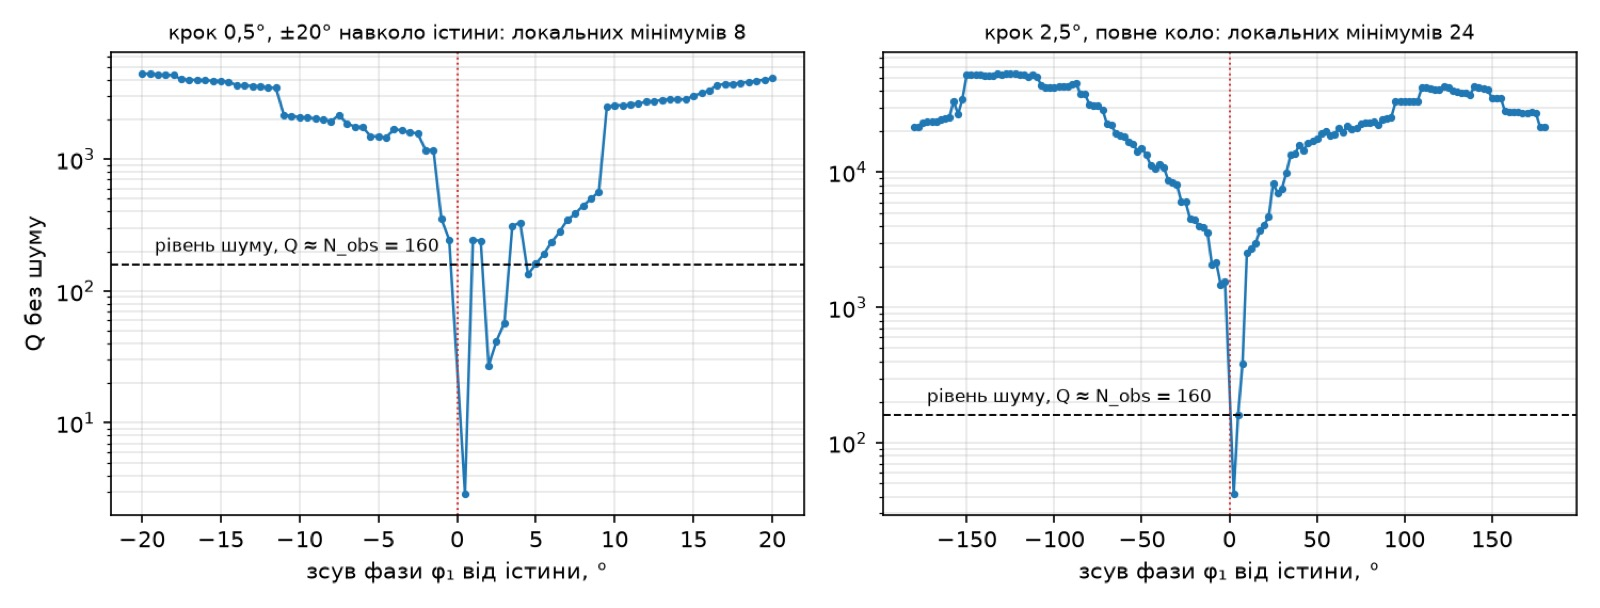
\includegraphics[width=\textwidth]{g07_c5_landscape.jpg}
\caption{Безшумова сума квадратів нев'язок $Q$ уздовж однієї фази $\varphi_1$ через істину (стенд A, екземпляр 0), логарифмічна шкала. Ліворуч: у межах $\pm20^\circ$ із кроком $0{,}5^\circ$ є 8 локальних мінімумів, і зсув на $0{,}5^\circ$ дає $Q=245$ в один бік і 2,9 в інший. Праворуч: повне коло, 24 мінімуми. Пунктир~--- рівень шуму $Q\approx N_{\mathrm{obs}}=160$. Власний розрахунок, код: \texttt{Our try/03-deep-dives/D3-poincare-inverse/c5/diag\_tokamap.py}, \texttt{guide/figures/g07\_c5\_landscape.py}.}
\label{fig:g07-c5}
\end{figure}

\begin{established}{E40 (post-hoc, на вердикт не впливала)}
Ландшафт нев'язки екскурсійного спостережуваного «скляний»: базовий фіт застрягає навіть поруч з істиною. Старт в істині лишається на місці ($Q/Q_{\mathrm{true}}=0{,}99$--$1{,}00$, тобто код коректний). Старт з істини $+5\,\%$ і $+10^\circ$ зупиняється при $Q/Q_{\mathrm{true}}=41$--$100$, а з $+20\,\%$ і $+45^\circ$~--- при 111--779. Механізм у рядку~46 \texttt{stand\_tokamap.py}: розмах~--- максимум по дискретних точках орбіти, тож малий зсув параметра змінює, \emph{яка} точка дає екстремум, і нев'язка стрибає (рис.~\ref{fig:g07-c5}). На стенді B скан пар фаз з кроком $30^\circ$ дав 8 і 14 локальних мінімумів, усі далеко від рівня шуму ($Q_0\ge2\,184\gg N_{\mathrm{obs}}=132$)~\cite{RegEst,g07C5}.
\end{established}

\paragraph{Що з цього випливає.} Задача Рівня~3 \emph{у цій постановці} (екскурсія як розмах і градієнтний фіт) не годиться як завдання базового рівня: команда без глобальної оптимізації чи сурогатної моделі не отримає нічого. Дві ідеї з \texttt{c5/README.md} \emph{не перевірені} і в реєстрі не стоять. Перша: висновок «складність задає спостережуване» може стосуватися лише згладженої (січної) задачі. Друга: гладше спостережуване (середнє чи квантиль замість розмаху, довші траси) може розгладити ландшафт і повернути задачу в межі базового фіту~\cite{g07C5}.

\section{Стан C5}\label{sec:g07-status}

\begin{itemcard}{R13 (була C5)}{закрито 2026-10-01: спростовано (реєстр) \quad·\quad \S\ref{sec:g07-c5test}}
Базовий нелінійний фіт не відновлює 3 амплітуди і 3 фази при 3\,\% шуму на жодному стенді (0 з 40, 0 з 3), хоча хибних мінімумів немає; ландшафт «скляний» (E40). Що лишилося від попередньої історії: VE21--VE25, VE30, VE31 як вимірювання локальної січної обумовленості; симплектичний багатомодовий стенд Tokamap (E35); залежність $\kappa$ від вибірки (17,9 в INVERSE проти 10,7 у скані мод для тих самих трьох мод). Межі, названі в INVERSE §4, теж лишаються: поле вакуумне, без відгуку плазми; один розряд і один кадр; слід на стінці без трасування многовидів~\cite{RegEst,RegConj,g07Inverse}.
\end{itemcard}

\begin{practicum}[обернена задача]
\textbf{Відтворити пілот} (з \texttt{fusion equilibrium challenge/starter}, $\approx$20~с, 40~с, 90~с): \texttt{.venv/bin/python "../../Our try/03-deep-dives/D3-poincare-inverse/tokamap.py"}, потім \texttt{multimode.py} і \texttt{identifiability.py}. \textbf{Стенд} (з \texttt{tokamak-3d-viz}, хвилини): \texttt{python src/run\_inverse.py --out data/inverse --quick}.

\textbf{Задача~1 (E31 чесно).} Поставте \texttt{N\_PHASE = 1} в \texttt{identifiability.py} і виміряйте підлогу на \emph{тій самій} одномодовій мапі. Яка частина «540$\times$» припадає на усереднення, а яка на зміну стенда?

\textbf{Задача~2 (R8 $\to$ вправа на валідацію).} Виведіть твірну функцію для суми мод (\S\ref{sec:g07-r8}) самостійно, виправте копію \texttt{multimode.py} (звірка: \texttt{multimode\_fixed\_check.py}, E35) і повторіть розділ «3. IDENTIFIABILITY» уже на симплектичній мапі. Чи лишаються спектри розрізненними над підлогою з 24 фазами?

\textbf{Перевірка C5} (з \texttt{fusion equilibrium challenge/starter}): \texttt{.venv/bin/python "../../Our try/03-deep-dives/D3-poincare-inverse/c5/run\_tokamap.py"} ($\approx$2~хв, 10 ядер) і \texttt{diag\_tokamap.py} ($\approx$1~хв); стенд B (\texttt{run\_viz.py}) іде $\approx$3~год.

\textbf{Задача~3 (після R13: гладке спостережуване).} Нелінійний фіт розмаху застрягає (\S\ref{sec:g07-c5test}). Замініть у копії \texttt{stand\_tokamap.py} розмах $\max-\min$ на гладшу величину (середнє $|\Psi-\Psi_0|$ або квантиль 90\,\% по орбіті) і повторіть \texttt{diag\_tokamap.py}. Чи зникають локальні мінімуми на розрізі по $\varphi_1$? Якщо так, запустіть \texttt{run\_tokamap.py} з новим спостережуваним. Це ще не гіпотеза реєстру: перед запуском запишіть критерії, як у \texttt{c5/THEORY.md}.
\end{practicum}

\chapter{Острови, хаос і помилка \texorpdfstring{$\sqrt q$}{√q}}\label{ch:g08}

Це найповчальніша історія проєкту. Хибний канонічний імпульс ($\psi$ замість $\psit$) дав
формулу ширини магнітного острова, завищену в $\sqrt q$ раз. Вимірювання чесно показали
«дефіцит» ширини, а ми двічі пояснили його фізикою: спершу дискретністю засіву, потім
стохастичним шаром сепаратриси. Лише коли гамільтоніан силової лінії вивели заново, дефіцит
зник: відношення «виміряно/теорія» стали $0{,}95$--$1{,}02$. Помилка не нова: це рецидив R4
батьківського реєстру \cite{RegEst}, який журнал верифікації впіймав ще 22.09 у чернетці
тексту (V-D3 \cite{RegVerif}). Тоді її виправили в документі, але не в коді. Реєстри
\cite{RegViz} зберігають усі проміжні пояснення як спростовані (VR12, VR15, VR16). Прочитайте
цей розділ як детектив: кожен крок у ньому був розумним.

\section{Стенд: навмисні острови в реальній рівновазі}\label{sec:g08-stand}

Усе рахується на одному кадрі DIII-D 203702 (кадр 75, $t=\SI{1760}{мс}$, $\qnf=3{,}6995$). В
осесиметрії силові лінії інтегровні, і перетин Пуанкаре дає рівно контури $\psi$ (E18). Тому
острови треба \emph{внести} збуренням потоку \cite{g08Physics}:
\begin{equation}\label{eq:g08-pert}
  \psi_{\text{total}}=\psi(R,Z)+\sum_k A_k\,g_k(\psiN)\cos\!\left(m_k\thetastar-n_k\varphi+\alpha_k\right),
  \qquad \Bvec=\grad\times(\psi_{\text{total}}\grad\varphi)+F\grad\varphi,
\end{equation}
де $g=\psiN^{m/2}$~--- «вакуумна» обвідна (розд.~\ref{ch:g09} покаже, що для реальних котушок
вона не годиться, VR14). Поле є ротором, тож $\grad\cdot\Bvec=0$ точно для будь-якого числа мод
(VE21, розд.~\ref{ch:g07}).

Перш ніж шукати острови, стенд пройшов перевірку ланцюга $\psi\to\Bvec$ (VE1--VE7). Пошук осі
збігається з EFIT до $\SI{0,0002}{мм}$ (VE1). LCFS набору є контуром $\psi$ з розкидом 0,022\,\%
(VE2). Калібрування $F$ лише за $\qnf$ дає $\Btor(\text{вісь})=\SI{1,927}{Тл}$ за реальних
1,9--2,1~Тл (VE3). Два способи обчислити $q$ збігаються до 0,001--0,16\,\% (VE4). Інтегратор
DOP853 зберігає $\psi$ до $10^{-7}$ за 200 обертів (VE5). Аналітичні похідні збурення збігаються
зі скінченними різницями до $10^{-7}$ (VE7). Дві ранні помилки варто запам'ятати. Резонанс
вимагає кута прямих силових ліній $\thetastar$, а не геометричного (VR1). Растеризація
$\cos m\thetastar$ на сітку $65\times65$ давала 2,4\,\% паразитної $m=1$ і фальшивий ланцюг на
$q=1$ (VE6, VR2). Ширина острова йде як корінь з амплітуди, тож кілька відсотків «бруду» дають
добре видимий острів. З двома модами 2/1 і 3/1 при амплітуді $10^{-3}$ розріз показує
\textbf{2 острови на $\psiN=0{,}752$ ($q=2$) і 3 на $\psiN=0{,}900$ ($q=3$)} (VE8).

\section{Як розпізнати острів: ланцюг спростувань класифікатора}\label{sec:g08-classifier}

Щоб порівнювати ширину з теорією, орбіти треба автоматично розкласти на регулярні, острівні
й хаотичні. Кожен шар класифікатора в \texttt{tokviz/analysis.py} з'явився після спростування
попереднього (VR8--VR13).

\paragraph{Крок 1. Число обертання (VR8 $\to$ VE16).} Просте середнє
$\nu=\langle\dd\pol/\dd\varphi\rangle$ за скінченним вікном несе осциляційну похибку
$\order{1/N}$, бо $\pol$ наростає вздовж D-подібної поверхні нерівномірно. На
\emph{інтегровному} полі це дало 50\,\% «хаотичних» орбіт (VR8). Заміна~--- зважене усереднення
Біркгофа з гладкою «шапочкою» $w(t)=\exp[-1/(t(1-t))]$. Вага разом з усіма похідними
занулюється на кінцях, тож на квазіперіодичній орбіті середнє збігається надполіноміально, а на
хаотичній не збігається зовсім (у докстрингу коду названо Das \& Yorke і Sander \& Meiss).
Так виміряне $\nu$ відтворює $1/q$ рівноваги до 0,03\,\%: це третій незалежний спосіб
дістати $q$ (VE16).

\code{viz/src/tokviz/analysis.py}{42}{57}{(ваги й зважене середнє Біркгофа)}

Рядки 42--51: вузли $t_i=(i+\frac12)/n$ лежать усередині $(0,1)$, тож $w$ ніде не ділить на
нуль. Нормування $\sum w_i=1$ робить результат справжнім середнім. Рядки 54--57: середнє вздовж
осі~1 (вздовж орбіти) рахується одним матричним множенням для всіх орбіт одразу.

\code{viz/src/tokviz/analysis.py}{81}{96}{(збіжність у десяткових цифрах)}

Рядки 88--92: $\nu$ за всією орбітою і за її першою половиною. Рядки 93--96: кількість
цифр, у яких вони збігаються, $-\log_{10}|\nu_{\text{full}}-\nu_{\text{half}}|/\nu_{\text{full}}$.
Поріг хаосу не вгадують, а калібрують на $A=0$, де система точно інтегровна: мінімум
5,14 цифри, медіана 6,66, поріг на декаду нижче, $4{,}14$ \cite{g08Analysis}.

\paragraph{Крок 2. Острів --- це захоплення $\nu$, а не екскурсія (VR9--VR13).} Перша ідея
«острівна орбіта має велику радіальну екскурсію $\psiN$» хибна в принципі (VR9). У фігурній
рівновазі екскурсія зростає до краю й для регулярних орбіт, а справжні острівні орбіти
($\nu=0{,}49999$) класифікувались як хаос. Правильна ознака~--- \emph{фазове захоплення}: у
смузі острова всі орбіти мають однакове $\nu=n/m$. Далі йде ланцюжок уточнень, і кожне
спростоване нульовим збуренням, де островів бути не може:
\begin{itemize}
  \item близькості до раціонального числа у вікні 2\,\% замало: на $A=0$ це дало 2 «острови» (VR10);
  \item додали взаємну узгодженість: $\nu$ членів смуги збігаються між собою до $2\cdot10^{-3}$;
  \item при 150 зернах сусіди мають майже однакове $\nu$ просто через гладкість профілю,
        і знову вийшло 2 «острови» на $A=0$ (VR13);
  \item додали безрозмірний \emph{тест пласкості}: розкид $\nu$ у смузі порівнюють зі
        зміною рівноважного $1/q$ на тому самому інтервалі $\psiN$.
\end{itemize}

\code{viz/src/tokviz/analysis.py}{133}{160}{(\texttt{find\_locked\_bands}: перевірка однієї смуги)}

Рядки 136--140: середнє $\nu$ смуги та її відносний розкид (тест VR10). Рядки 142--152: тест
пласкості (VR13). \texttt{expected}~--- на скільки змінилось би $\nu$ на ширині смуги без
захоплення. Тест вирішальний лише тоді, коли ця зміна помітна (рядок~151). Рядки 154--160:
смуга з кількох орбіт або одна дуже точно захоплена орбіта (\texttt{solo\_tol}).

\paragraph{Крок 3. Порядок перевірок (VR11).} Острівна орбіта має другу, повільну частоту~---
лібрацію навколо O-точки~--- і тому за Біркгофом збігається \emph{гірше} за KAM-орбіту. Якщо
спершу перевірити збіжність, острів завжди читається як хаос. Тому захоплення перевіряється
першим:

\code{viz/src/tokviz/analysis.py}{193}{221}{(тіло \texttt{classify})}

Рядки 193--200: цифри збіжності, $\nu$ і смуги захоплення. Рядки 202--208: острівними стають
члени смуг, які вижили й мають хоч якусь збіжність (\texttt{stability\_digits}). Рядок 210:
хаос~--- лише серед \emph{не}острівних орбіт. Рядки 213--221: мітки й частка хаосу.
Результат видно на рис.~\ref{fig:g08-ab}: хаотичні орбіти сидять рівно на $\nu=1/2$ і $\nu=1/3$,
хоча класифікатор нічого не знає про резонанси (VE17).

\begin{figure}[ht]
  \centering
  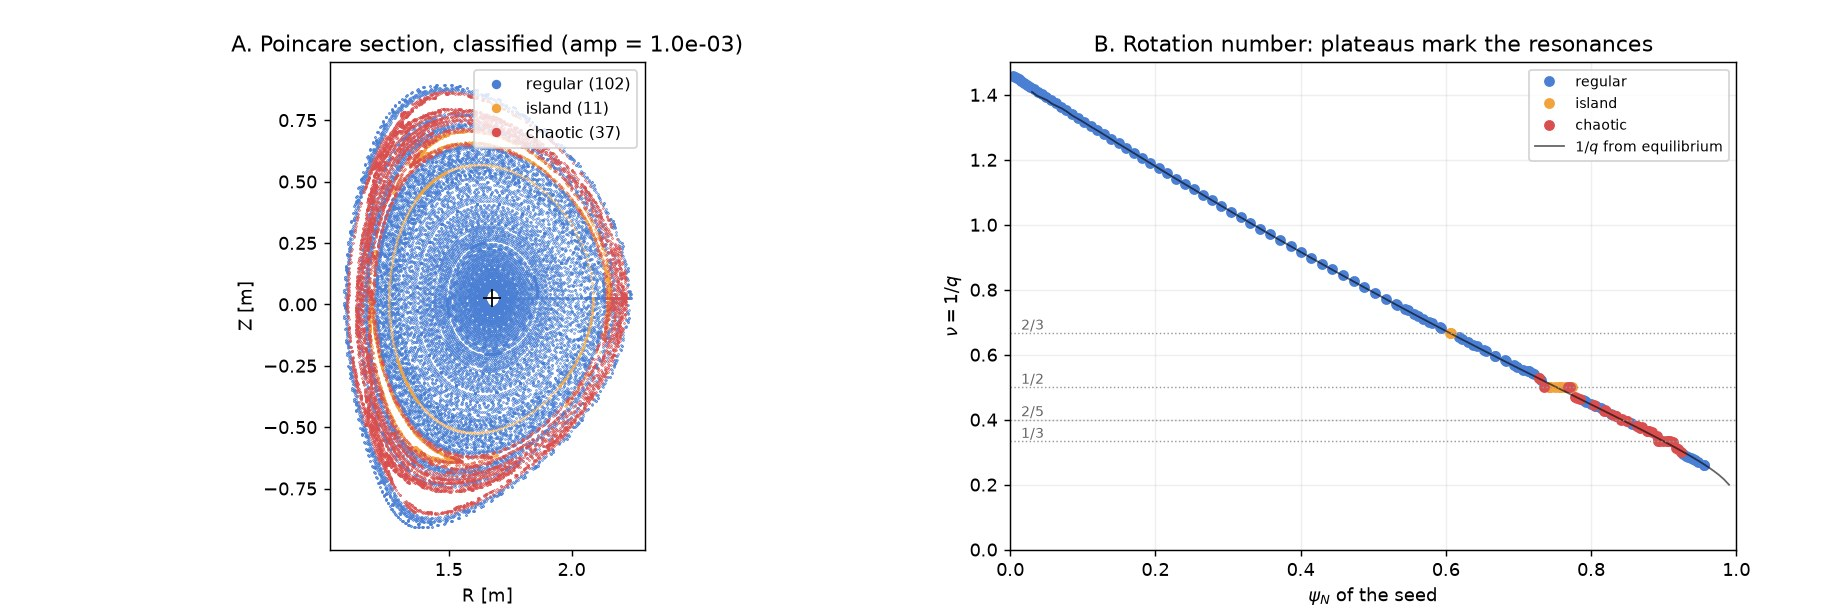
\includegraphics[width=\textwidth]{g08_poincare_after_AB.jpg}
  \caption{Класифікований перетин при $A=10^{-3}$ (A) і профіль $\nu(\psiN)$ проти $1/q$
  рівноваги (B), DIII-D 203702. Свіжий прогін 2026-09-29 з виправленою формулою. Дві
  помаранчеві орбіти на $\nu=2/3$ ($\psiN\approx0{,}61$)~--- смуга 3/2, яку класифікатор
  знаходить і при $A=0$ (за \texttt{data/analysis/analysis.json}). Це прояв VQ4
  (розд.~\ref{sec:g08-vq4}). Власний розрахунок, код: \texttt{tokamak-3d-viz/src/run\_analysis.py}.}
  \label{fig:g08-ab}
\end{figure}

\section{Ширина острова: маятник і канонічна пара}\label{sec:g08-pendulum}

\begin{derivation}[ширина острова з гамільтоніана силової лінії]
Для $\Bvec=\grad\psi\times\grad\varphi+F\grad\varphi$ ($\psi$~--- полоїдальний потік на радіан)
рівняння силових ліній є гамільтоновою системою з 1,5 ступеня вільності (E19,
\cite{Escande2024}): час~--- $\varphi$, координата~--- $\thetastar$,
\textbf{імпульс~--- тороїдальний потік $\psit$}, \textbf{гамільтоніан~--- полоїдальний потік $\psi$}:
\begin{equation}\label{eq:g08-ham}
\frac{\dd\thetastar}{\dd\varphi}=\frac{\pa\psi}{\pa\psit}=\frac1q\equiv\nu,\qquad
\frac{\dd\psit}{\dd\varphi}=-\frac{\pa\psi}{\pa\thetastar},\qquad \dd\psi=\frac{\dd\psit}{q}.
\end{equation}
Нехай $\psi=\psi_0(\psit)+A\cos\xi$ з резонансною фазою $\xi=m\thetastar-n\varphi+\alpha$. Біля
резонансу $\nu(\psit^{\text{res}})=n/m$ розкладаємо $\nu$ до першого порядку й дістаємо маятник:
\begin{equation}\label{eq:g08-pend}
\frac{\dd\xi}{\dd\varphi}=m\,\nu'\,(\psit-\psit^{\text{res}}),\qquad
\frac{\dd\psit}{\dd\varphi}=mA\sin\xi,\qquad
\nu'=\frac{\dd\nu}{\dd\psit}=-\frac{1}{q^2}\frac{\dd q}{\dd\psi}\frac{\dd\psi}{\dd\psit}=-\frac{\dd q/\dd\psi}{q^3}.
\end{equation}
Це рівняння руху для $K=\frac12 m\nu' p^2+mA\cos\xi$, $p=\psit-\psit^{\text{res}}$. На
сепаратрисі $\frac12|m\nu'|p_{\max}^2=2|mA|$, звідки повна ширина $4\sqrt{A/|\nu'|}$ (множник $m$
скорочується). Ширина в $\psi$ у $q$ разів менша за ширину в $\psit$:
\begin{equation}\label{eq:g08-W}
W_{\psi}=\frac1q\cdot4\sqrt{\frac{Aq^3}{|\dd q/\dd\psi|}}=4\sqrt{\frac{Aq}{|\dd q/\dd\psi|}}
\quad\Longrightarrow\quad
W=4\sqrt{\frac{\varepsilon q}{|\dd q/\dd\psiN|}},\qquad \varepsilon=\frac{A}{|\psib-\psiax|}.
\end{equation}
Друга форма~--- та сама формула в нормованому потоці: $A$ і $\dd q/\dd\psi$ масштабуються з
діапазоном потоку однаково.

\emph{Де була помилка.} Якщо вважати імпульсом сам $\psi$, тобто писати
$\dd\psi/\dd\varphi=mA\sin\xi$, то той самий маятник дає
$W=4\sqrt{A/|\dd\nu/\dd\psi|}=4\sqrt{Aq^2/|\dd q/\dd\psi|}$. Насправді
$\dd\psi/\dd\varphi=\nu\,\dd\psit/\dd\varphi$: у рівнянні для $\dot\psi$ бракує множника $1/q$, і
ширина виходить завищеною в $\sqrt q$ раз. Для $q=2$ це 41\,\%, для $q=3$~--- 73\,\%.
\end{derivation}

Сьогодні формула в коді така:

\code{viz/src/tokviz/perturbation.py}{197}{230}{(\texttt{island\_width\_psin}, виправлена версія)}

Рядки 198--224: докстринг повторює виведення~\eqref{eq:g08-ham}--\eqref{eq:g08-W}, щоб наступний
читач не мусив його відновлювати. Рядки 225--226: запис про стару формулу (правило «нічого не
зникає мовчки» діє й у коді). Рядки 228--230: власне обчислення; до 2026-09-29 тут стояло
\verb|eps*q**2| \cite{g08Changes}.

Перекриття двох ланцюгів оцінює параметр Чирикова
$S=(W_1+W_2)/(2|\psi_{N,1}-\psi_{N,2}|)$ (функція \texttt{chirikov}, рядки 233--242 того самого
файлу; у докстрингу прямо сказано, що $S\ge1$~--- евристика, а не теорема). Для стенда при
$A=10^{-3}$: мода 2/1 має $\psiN=0{,}7520$, $\varepsilon=7{,}52\cdot10^{-4}$,
$\dd q/\dd\psiN=4{,}44$, $W=0{,}0736$. Мода 3/1 має $\psiN=0{,}9001$,
$\varepsilon=8{,}54\cdot10^{-4}$, $\dd q/\dd\psiN=10{,}70$, $W=0{,}0619$. Звідси
$S=\mathbf{0{,}458}$ (VE9; до виправлення $W=0{,}1041/0{,}1072$ і $S=0{,}714$).

\section{Історія хибного пояснення}\label{sec:g08-story}

\paragraph{Вимір.} Ширину острова міряє \texttt{measured\_island\_width}: це об'єднання
радіальних екскурсій орбіт, захоплених на резонансі, тобто смуга, яку перетин справді показує.

\code{viz/src/tokviz/analysis.py}{224}{241}{(виміряна ширина ланцюга)}

Рядки 231--235: члени смуг саме цього резонансу з міткою «острів». Рядки 238--241: ширина~---
розмах $\psiN$ уздовж \emph{траєкторій} (а не лише початкових зерен), плюс центр і кількість
орбіт.

\begin{refuted}{VR12}
«Дефіцит виміряної ширини пояснюється дискретністю засіву.» При 56 зернах (крок 0,0215)
поправка $W_{\text{теор}}-2\Delta\psi$ чисельно збігалася з виміром, і це виглядало переконливо.
Після згущення до кроку 0,003--0,004 біля резонансів поправка стала нікчемною, а відношення
0,72 лишилося. Збіг при 56 зернах був випадковим.
\end{refuted}

\begin{refuted}{VR16}
«Дефіцит (0,59--0,74)~--- це стохастичний шар сепаратриси, що з'їдає регулярне ядро острова.»
Це була \emph{опублікована} інтерпретація у VE18 і «справжня причина» у VR12. Розріз упоперек
$q=2$ справді показує тонкі хаотичні шари обабіч захопленого ядра $\psiN\in[0{,}7429;\,0{,}7739]$
з $\nu=0{,}50000$. Але пояснення не витримує двох перевірок. Відношення не залежало від
амплітуди, хоча шар, що росте з $S$, мав би давати таку залежність. Зате для кожної моди воно
збігалося з $1/\sqrt q$: $1/\sqrt2=0{,}71$, $1/\sqrt3=0{,}58$.
\end{refuted}

Саме останнє спостереження мало насторожити: безрозмірне число, яке залежить лише від $q$
резонансу,~--- підпис помилки у формулі, а не фізики. Помилку знайшов координатор методички під
час написання розд.~2 методички (знахідка N1 \cite{g08Coord}). Формулу виправили 2026-09-29.

\begin{refuted}{VR15}
«Ширину острова можна рахувати, беручи $\psi$ за канонічний імпульс»:
$W=4\sqrt{\varepsilon q^2/|\dd q/\dd\psi|}$. Це повторення R4 батьківського реєстру.
Канонічна пара~--- $(\thetastar,\psit)$, гамільтоніан~--- $\psi$ (E19). Виправлено в
\texttt{perturbation.island\_width\_psin} і \texttt{coilfield.CoilPerturbation.calibrate\_to\_island\_width}.
\emph{Не} оновлено: \texttt{data/bake01} і рендери Blender досі несуть старі $W$ і $S$.
\end{refuted}

Ті самі вимірювання (вихідний засів, збережений у \texttt{data/analysis\_pre\_fix\_2026-09-29/})
переоцінено новою формулою. Самі вимірювання від формули не залежать
(табл.~\ref{tab:g08-ratios}, рис.~\ref{fig:g08-cd}).

\begin{table}[ht]
\centering\footnotesize\setlength{\tabcolsep}{4pt}
\caption{Виміряна ширина острова проти маятникової: до і після виправлення
(\texttt{docs/ANALYSIS.md} §2.2; звірено з обома файлами \texttt{analysis.json})}
\label{tab:g08-ratios}
\begin{tabular}{@{}llcccccc@{}}
\toprule
$A$ & мода & $W_{\text{вим}}$ & $W_{\text{стар}}$ & вим./стар. & $W_{\text{нов}}$ & вим./нов. & $S$: стар.\,$\to$\,нов.\\
\midrule
$5\cdot10^{-4}$ & 2/1 & 0,0492 & 0,0736 & 0,67 & 0,0520 & \textbf{0,95} & 0,505\,$\to$\,0,324\\
$10^{-3}$ & 2/1 & 0,0752 & 0,1041 & 0,72 & 0,0736 & \textbf{1,02} & 0,714\,$\to$\,0,458\\
$10^{-3}$ & 3/1 & 0,0628 & 0,1072 & 0,59 & 0,0619 & \textbf{1,01} & 0,714\,$\to$\,0,458\\
$2\cdot10^{-3}$ & 2/1 & 0,1044 & 0,1472 & 0,71 & 0,1041 & \textbf{1,00} & 1,009\,$\to$\,0,647\\
$4\cdot10^{-3}$ & 3/1 & 0,1578 & 0,2145 & 0,74 & 0,1238 & 1,27$^{*}$ & 1,427\,$\to$\,0,915\\
\midrule
\multicolumn{8}{@{}l}{Трасування сепаратриси без класифікатора, одна мода, $A=10^{-3}$:
\textbf{0,983} (2/1), \textbf{0,996} (3/1) від нової формули}\\
\bottomrule
\end{tabular}\\[2pt]
{\footnotesize $^{*}$Поза маятниковим режимом: острів 3/1 сягає $\psiN\approx0{,}96$, $S\approx0{,}9$,
смуга з двох орбіт.}
\end{table}

\begin{figure}[ht]
  \centering
  \begin{subfigure}{0.82\textwidth}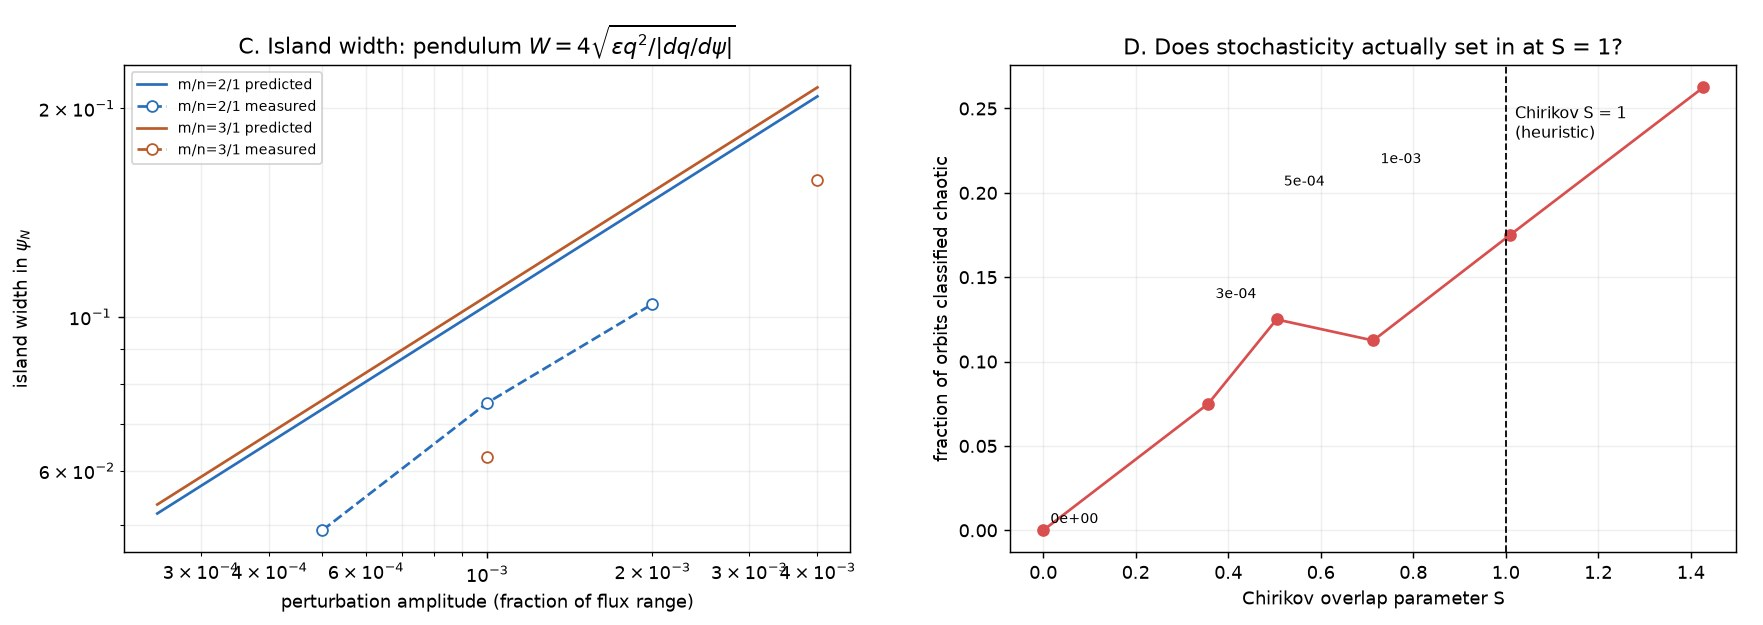
\includegraphics[width=\linewidth]{g08_poincare_before_CD.jpg}
  \caption{до виправлення: $W=4\sqrt{\varepsilon q^2/|\dd q/\dd\psi|}$}\end{subfigure}\\[3pt]
  \begin{subfigure}{0.82\textwidth}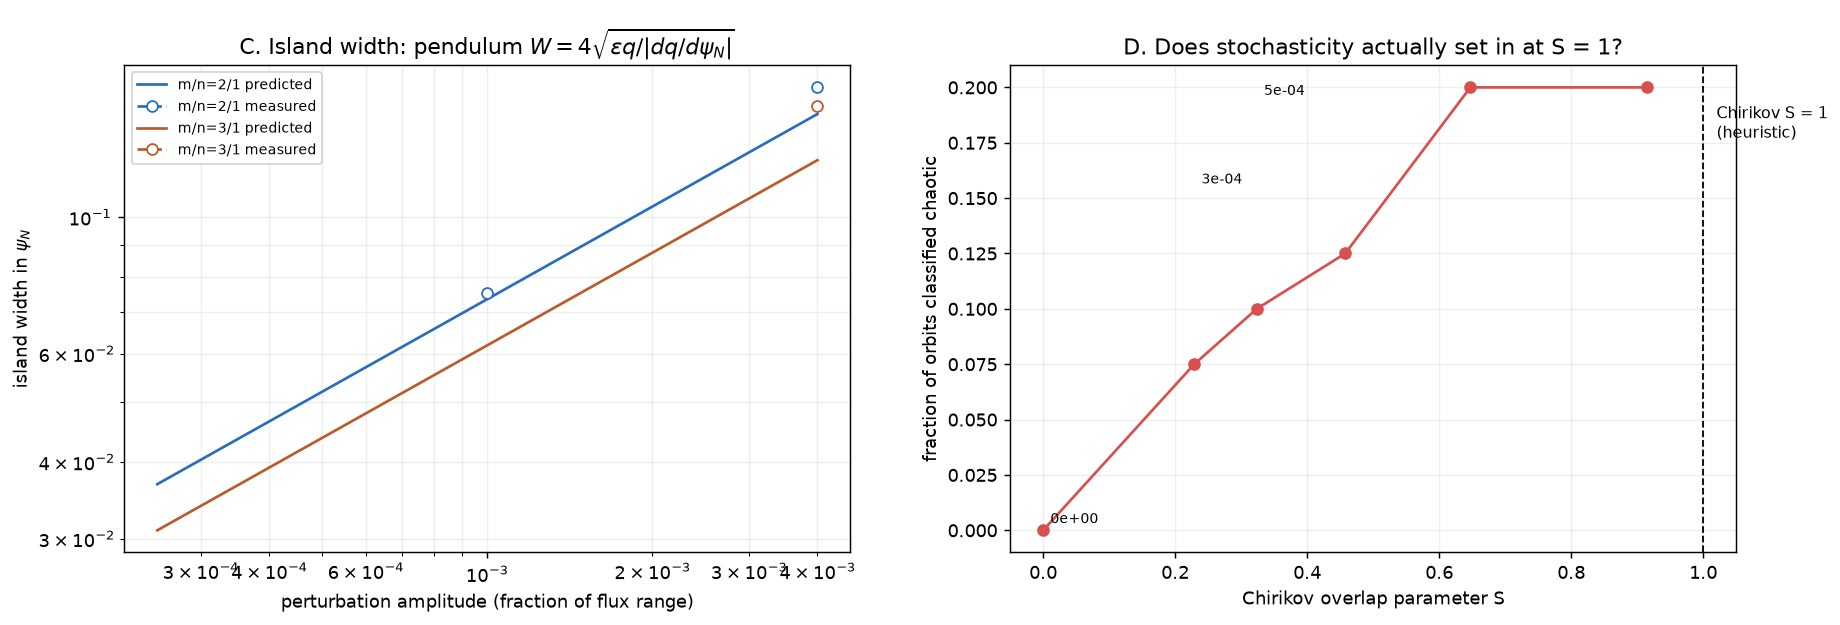
\includegraphics[width=\linewidth]{g08_poincare_after_CD.jpg}
  \caption{після: $W=4\sqrt{\varepsilon q/|\dd q/\dd\psiN|}$ (свіжий прогін)}\end{subfigure}
  \caption{Ширина острова проти амплітуди (ліворуч; лінії~--- теорія, кружки~--- вимір) і частка
  хаотичних орбіт проти $S$ Чирикова (праворуч). До виправлення всі виміряні точки лежать нижче
  теорії на сталий множник $\approx1/\sqrt q$. Після виправлення вони лягають на лінії, а скан
  уже не досягає $S=1$. У свіжому прогоні класифікатор не знайшов смугу 2/1 при $5\cdot10^{-4}$ і
  $2\cdot10^{-3}$ (VQ4). Власний розрахунок, код: \texttt{tokamak-3d-viz/src/run\_analysis.py}
  (\texttt{data/analysis\_pre\_fix\_2026-09-29/} і \texttt{data/analysis/}).}
  \label{fig:g08-cd}
\end{figure}

Вирішальним став незалежний тест без класифікатора. Він трасує одну моду й вважає острівною
орбіту, у якої резонансна фаза $\xi=m\thetastar-n\varphi$ лібрує (розмах менший за $2\pi$):

\code{viz/tests/test_physics.py}{139}{161}{(\texttt{test\_island\_width\_matches\_traced\_separatrix})}

Рядки 140--145: одна мода, її резонанс, $\varepsilon$ і передбачена $W$. Рядки 147--150:
20 зерен на зовнішній середній площині в межах $\pm0{,}75W$ і трасування на 50 обертів. Рядки
151--153: критерій лібрації, незалежний від $\nu$ і від класифікатора. Рядок 155: зерна мусять
охоплювати острів з обох боків. Рядки 158--161: вимір має бути в межах 10\,\% від нової
формули і відрізнятися від старої більш ніж на 20\,\%. Отже, тест здатен розрізнити
$\sqrt q$. Повторний запуск цього коду для путівника (2026-09-29) дав $W_{\text{вим}}=0{,}0723$
проти $0{,}0736$ (2/1, відношення $0{,}983$, 8 захоплених орбіт) і $0{,}0617$ проти $0{,}0619$
(3/1, $0{,}996$, 5 орбіт); реєстрові числа відтворились.

\begin{established}{VE18 (переформульовано 2026-09-29)}
Маятникова формула (виправлена) справджується: виміряна ширина збігається з передбаченою до
0--5\,\% при $A\le2\cdot10^{-3}$. Тонкі стохастичні шари біля сепаратриси є, але траєкторії
захоплених орбіт (0,0752) заповнюють усю передбачену сепаратрису (0,0736). «Три ширини» старого
тексту зводяться до двох: розкид \emph{зерен} ядра (0,0310; зерна стоять на одній лінії при
одній фазі) і ширина сепаратриси.
\end{established}

\section{Хаос і критерій Чирикова}\label{sec:g08-chirikov}

Виправлення змінило вісь $S$, але не частки хаосу: їх класифікатор міряв незалежно від формули
(табл.~\ref{tab:g08-chaos}).

\begin{table}[ht]
\centering\small
\caption{Частка хаотичних орбіт (VE19, VE20, VE33; \texttt{docs/ANALYSIS.md} §2.3)}
\label{tab:g08-chaos}
\begin{tabular}{@{}lccccc@{}}
\toprule
$A$ & $S$ стар.\,$\to$\,нов. & незміщена (80 рівномірних) & усі 150 зерен & завищення & свіжий прогін\\
\midrule
0 & 0 & 0,000 & 0,000 & --- & 0,000\\
$2{,}5\cdot10^{-4}$ & 0,357\,$\to$\,0,229 & 0,075 & 0,133 & 1,78$\times$ & 0,075\\
$5\cdot10^{-4}$ & 0,505\,$\to$\,0,324 & 0,125 & 0,200 & 1,60$\times$ & 0,100\\
$10^{-3}$ & 0,714\,$\to$\,0,458 & 0,113 & 0,213 & 1,90$\times$ & 0,125\\
$2\cdot10^{-3}$ & 1,009\,$\to$\,0,647 & 0,175 & 0,300 & 1,71$\times$ & 0,200\\
$4\cdot10^{-3}$ & 1,427\,$\to$\,0,915 & 0,263 & 0,413 & 1,57$\times$ & 0,200\\
\bottomrule
\end{tabular}
\end{table}

\begin{itemize}
\item \textbf{VE9.} $S=0{,}458<1$, і поверхні між ланцюгами справді виживають. Це один
      узгоджений випадок, а не доказ евристики. Після виправлення висновок лише посилився.
\item \textbf{VE19.} Хаос існує задовго до $S=1$: вимірна частка є вже при $S=0{,}229$. Друга
      половина старого заголовка («різкого порогу при $S=1$ немає») знята: з виправленою формулою
      скан \emph{не досягає} $S=1$, тож перехід через одиницю цими даними не перевірено. Для
      $S\ge1$ потрібні $A\gtrsim5\cdot10^{-3}$.
\item \textbf{VE20.} Зерна, згущені біля резонансів, завищують частку хаосу в 1,6--1,9 раза.
      Тому статистику хаосу рахують лише на рівномірних 80 зернах, а згущені 70 йдуть тільки на
      вимір ширини. Методологічний урок: будь-яка «частка стохастичного об'єму», порахована на
      зернах біля резонансів, завищена приблизно вдвічі.
\item \textbf{VE33 (закрито VC5).} Немонотонність частки при 40 зернах (0,275\,$\to$\,0,200) була
      шумом вибірки. Одна орбіта з 80~--- це 1,25\,\%, тож западина 0,125\,$\to$\,0,113 незначуща.
      «Підтверджено» тут означає «у межах статистики однієї-двох орбіт».
\end{itemize}

Застереження, що стоїть на всіх числах: \emph{вакуумний} перетин переоцінює стохастичність, бо
плазма екранує резонансні компоненти. Частки в табл.~\ref{tab:g08-chaos}~--- верхня межа.

\section{Що лишилось відкритим: VQ4}\label{sec:g08-vq4}

Свіжий прогін тією самою командою змінив засів: згущення тепер ставиться за меншою
передбаченою шириною. Поріг хаосу став $3{,}88$ цифри замість $4{,}14$. Смугу 2/1 при $10^{-3}$
знайдено з тим самим відношенням $1{,}02$. Але при $5\cdot10^{-4}$ і $2\cdot10^{-3}$ класифікатор
\emph{не виділив} жодної захопленої смуги 2/1 (при $2{,}5\cdot10^{-4}$~--- лише плато), а при $A=0$
позначив 2 орбіти як «острови». Уточнення реєстру 2026-09-29: хибна \emph{смуга} одна~--- 3/2
(2 орбіти, розкид $\nu$ $1{,}2\cdot10^{-3}$), і вона з'являється при всіх $A\le10^{-3}$; 5/2 дає
лише $\nu$-плато шириною 0,0011, смугою не стає. Тобто тест пласкості, введений після VR13, сам
виявився чутливим до щільності засіву.

\begin{conjecture}{VQ4 (відкрите питання реєстру)}
Чи надійний класифікатор островів (тест пласкості $\nu$) при новому засіві? Висновки про ширину
(VE18) спираються на вихідний засів і незалежний тест лібрації, тож їх це не зачіпає. Проте
свіжий \texttt{analysis.json}~--- гірше джерело для VE19 і VE33, а \texttt{run\_parasitic}
після виправлення не перезапускався. \emph{Закриє:} тест пласкості, що на $A=0$ дає 0 островів
і знаходить 2/1 на всіх амплітудах при обох засівах.
\end{conjecture}

\begin{practicum}[відтворити й зламати]
Потрібні дані DIII-D (\texttt{TOKVIZ\_DATA\_DIR} на теку з \texttt{d3d\_shot\_203702.parquet}) і
Python зі scipy (підходить venv конкурсу \texttt{fusion equilibrium challenge/starter/.venv}).
\begin{enumerate}
\item \verb|python tests/test_physics.py| --- усі фізичні тести стенда, зокрема тест лібрації.
\item Поверніть у \texttt{island\_width\_psin} множник \verb|q_res**2| і запустіть тест знову. Він
      має впасти на рядку «measured \ldots vs predicted». Це і є регресійний захист від R4.
\item \verb|python src/run_analysis.py --out data/analysis --n-seeds 80 --n-refine 35| відтворює
      рис.~\ref{fig:g08-cd}. Додайте \verb|--amps 0,5e-3,1e-3,5e-3,8e-3|, щоб уперше перевірити
      поведінку при $S\ge1$ (відкрито після VE19).
\item Задача для VQ4: змініть \texttt{flatness} чи умову рядка~151 у \texttt{find\_locked\_bands}
      так, щоб при $A=0$ було 0 островів для \emph{обох} засівів. Засів задають
      \verb|--n-refine| і \verb|--refine-span|.
\end{enumerate}
\end{practicum}

\paragraph{Мораль.} Помилку в канонічному імпульсі проєкт уже раз спростував (R4, V-D3), і все ж
вона повернулася в коді. Її двічі «пояснили» фізикою, бо кожне пояснення правдоподібне локально.
Тривогу мали викликати два сигнали: безрозмірне відношення, яке не залежить від амплітуди, і його
збіг із простим числом ($1/\sqrt q$). Врятували її три речі: незалежний тест, реєстр, де старі
пояснення не стираються, і повторне виведення з перших принципів.

\chapter{Поле реальних котушок}\label{ch:g09}

Стенд розд.~\ref{ch:g08} вносить збурення аналітично, з радіальною обвідною $g=\psiN^{m/2}$.
Вона росте до краю, як і належить вакуумному полю зовнішніх котушок. Але чи схожа вона на поле
\emph{справжнього} масиву RMP-котушок (resonant magnetic perturbation)? Реєстр візуалізації
записав це як здогадку VC1 з критерієм спростування «порівняння з полем I-котушок DIII-D за
Біо--Саваром» і вартістю «$\sim$день» \cite{RegViz}. Розділ розповідає, як здогадку спростовано
(VR14), що довелося побудувати натомість і яку помилку представлення поля ми зробили дорогою.
Та помилка~--- родичка R8 батьківського реєстру (розд.~\ref{ch:g07}).

\section{Біо--Савар, перевірений проти аналітики}\label{sec:g09-bs}

Масив I-котушок моделюється прямокутними «рамками» на циліндрі $R=R_{\text{coil}}$: два ряди по
6 котушок, струм у котушці $j$ зважено як $\cos(n\varphi_j)$ (\texttt{rmp\_coils.icoil\_array}).
Поле рахує сума внесків прямих відрізків:

\code{viz/src/tokviz/rmp_coils.py}{76}{99}{(\texttt{biot\_savart})}

Рядки 83--86: кожна петля~--- ламана з вершин \texttt{v}; відрізок від $\vect a$ до $\vect b$.
Рядки 87--92: точки обробляються порціями (\texttt{chunk}), щоб масив «точки $\times$ відрізки»
вмістився в пам'ять. Рядки 93--96: замкнена формула поля скінченного прямого відрізка,
$\dd\vect l\times\vect r_1\,(|\vect r_1|+|\vect r_2|)/[|\vect r_1||\vect r_2|(|\vect r_1||\vect r_2|+\vect r_1\cdot\vect r_2)]$.
Точки на самому провіднику (знаменник $\to0$) відкидаються. Рядок 98: множник $\mu_0I/4\pi$.

\begin{established}{VE27}
Поле на осі кругової петлі збігається з $\mu_0Ia^2/[2(a^2+z^2)^{3/2}]$ до 4 знаків при
$z/a=0;\ 0{,}5;\ 1;\ 2$ (тест \nolinkurl{test_biot_savart_matches_analytic_loop}). Масив із 6
котушок дає домінантну $n=3$ і першу бічну смугу $n=9$ на рівні 12\,\%. Саме таке аліасування
$n=3\pm6k$ має давати дискретний масив.
\end{established}

Дві помилки дорогою, обидві записані \cite{g07Campaign}. Перша (VE28): поле масиву спершу
зондували на магнітній осі при $Z=0$, де внески верхнього й нижнього рядів взаємно знищуються за
симетрією, і отримали абсурдні $4\cdot10^{-23}$~Тл. На краю плазми ($R=2{,}05$, $Z=0{,}3$) те саме
поле дає rms $2{,}8\cdot10^{-7}$~Тл/А. Друга: струми спочатку задавали бінарним знаком
$\operatorname{sign}(\cos n\varphi)$, а такий меандр сам породжує зайві гармоніки. Тепер у коді
стоїть синусоїдальне ваговання з коментарем, чому саме так (\texttt{rmp\_coils.py}, рядки 63--67).

\section{VC1: чи схожа обвідна на поле котушок}\label{sec:g09-vc1}

\paragraph{Метод.} Беремо нормальну до магнітної поверхні компоненту поля
$b_n=\vect B\cdot\grad\psi/|\grad\psi|$ і розкладаємо її в ряд Фур'є за $\thetastar$ і $\varphi$.
Модуль резонансної гармоніки $|b_{mn}(\psiN)|$ порівнюємо з тим самим числом для аналітичного
стенда. Амплітуду нормують, бо перевіряється лише \emph{форма} профілю.

\code{viz/src/run_coil_compare.py}{66}{82}{(\texttt{resonant\_harmonic})}

Рядок 71: точки поверхні рівномірно за $\thetastar$ і нормаль (функція \texttt{surface\_grid},
рядки 44--63). Рядки 76--78: $b_n$ на сітці $\varphi\times\thetastar$ для будь-якого поля, заданого
функцією. Тому одна процедура міряє і котушки, і стенд. Рядки 80--81: проєкція на
$\exp[-\mathrm i(m\thetastar-n\varphi)]$ дає комплексну амплітуду гармоніки.

Профіль стискаємо до одного числа~--- показника $p$ у $|b_{mn}|\propto\psiN^{p}$ на зовнішній
частині $\psiN\ge0{,}45$. Якщо обвідна чесна, для котушок має вийти $p$ поблизу
показника самого стенда:

\code{viz/src/run_coil_compare.py}{160}{171}{(\texttt{fit\_exponent})}

Рядок 168: лише скінченні додатні точки зовнішньої області. Рядок 171: нахил прямої в
логарифмічних координатах. Оскільки опубліковані розміри I-котушок у джерелах різняться,
порівняння повторено для шести варіантів геометрії (рядки 110--117 того самого файлу): номінал
$R_{\text{coil}}=2{,}184$~м, $z_c=0{,}754$~м, висота $0{,}5$~м, радіус $\pm10\,\%$, висота центру
$\pm25\,\%$ і «високі» котушки 0,8~м.

\begin{table}[ht]
\centering\small
\caption{Показник $p$ і кореляція профілів котушок зі стендом. Дані:
\texttt{coil\_compare.json}, звірено для путівника}
\label{tab:g09-exp}
\begin{tabular}{@{}lcccc@{}}
\toprule
& \multicolumn{2}{c}{$m/n=2/1$} & \multicolumn{2}{c}{$m/n=3/1$}\\
варіант & $p$ & кор. & $p$ & кор.\\
\midrule
номінал & $-0{,}08$ & 0,61 & 2,44 & 0,94\\
$R-10\,\%$ & 0,78 & 0,63 & 1,55 & 0,37\\
$R+10\,\%$ & $-0{,}34$ & 0,25 & 0,94 & 0,91\\
$z_c-25\,\%$ & $-0{,}93$ & $-0{,}45$ & 0,07 & 0,71\\
$z_c+25\,\%$ & 1,01 & 0,95 & 2,96 & 0,77\\
високі & $-0{,}48$ & 0,14 & 0,86 & 0,86\\
\midrule
стенд, $\psiN^{m/2}$ (та сама метрика) & 0,73 & --- & 1,23 & ---\\
\bottomrule
\end{tabular}
\end{table}

\begin{figure}[ht]
  \centering
  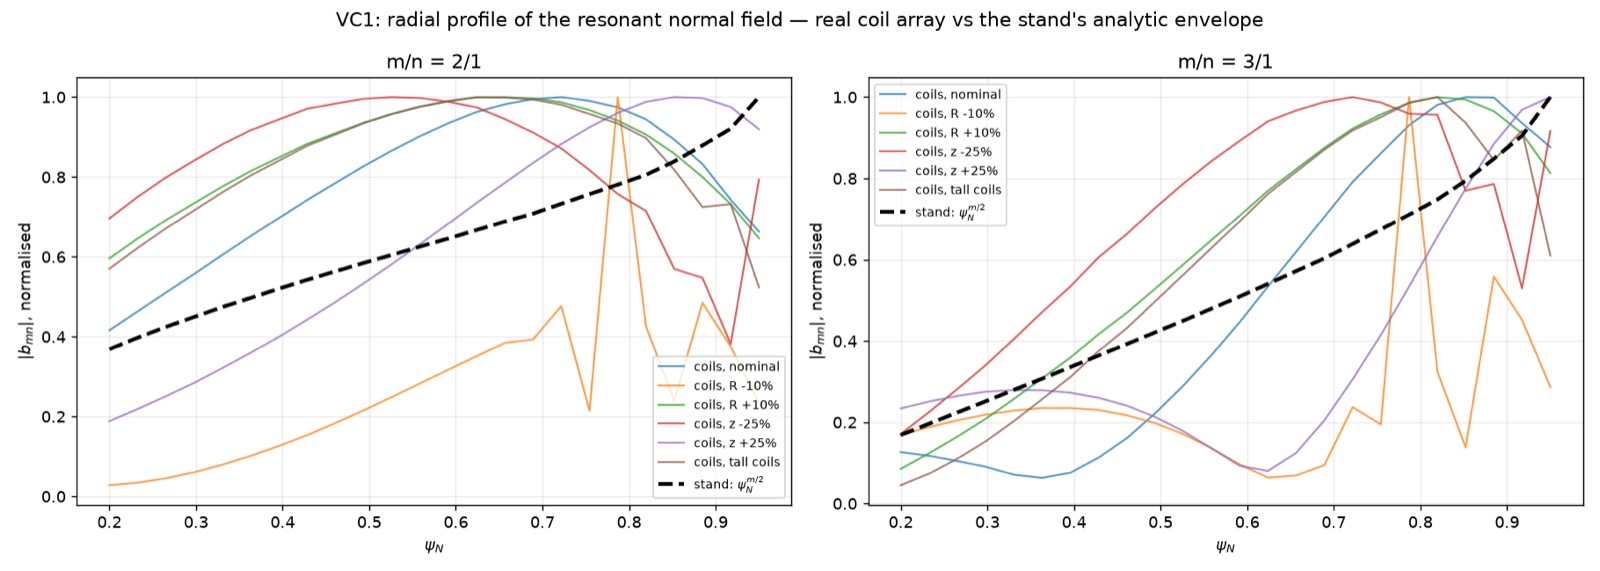
\includegraphics[width=\textwidth]{g09_coil_compare.jpg}
  \caption{Нормований радіальний профіль резонансної нормальної компоненти: шість варіантів
  масиву котушок (кольорові) проти обвідної стенда $\psiN^{m/2}$ (чорна штрихова). Жоден варіант
  котушок не монотонний назовні. Власний розрахунок, код:
  \texttt{tokamak-3d-viz/src/run\_coil\_compare.py}.}
  \label{fig:g09-coil}
\end{figure}

\begin{refuted}{VC1 $\to$ VR14}
«Обвідна $\psiN^{m/2}$ достатньо близька до поля реальних RMP-котушок.» Показник степеня для
котушок гуляє від $-0{,}93$ до $+1{,}01$ для $m=2$ (обвідна в тій самій метриці дає 0,73) і від
0,07 до 2,96 для $m=3$ (обвідна 1,23). Кореляція профілів коливається від $-0{,}45$ до $+0{,}95$.
Розкид задають радіус і висота масиву~--- саме ті параметри, які в публікаціях подають
по-різному. Жоден варіант котушок не монотонний назовні, тоді як $\psiN^{m/2}$ монотонна за
побудовою. \emph{Наслідок:} обвідна придатна для \emph{візуалізації}, але не для кількісних
тверджень про реальні RMP-експерименти.
\end{refuted}

Зауважте формулювання «придатна для візуалізації». Спростування не викидає інструмент, а звужує
його застосовність. Це записано в реєстрі, щоб рендер стенда ніхто не прочитав як модель
конкретного розряду з котушками.

\paragraph{Побічна перевірка: паразитні гармоніки (VC2 $\to$ VE26).} Ця сама кампанія закрила й
сусідню здогадку. Збурення містило \emph{лише} 2/1 і 3/1. По 44 орбіти засіяно в смузі
$\pm0{,}045$ навколо семи кандидатних резонансів, трасування на 150 обертів. Керовані ланцюги
знайдено ($W=0{,}0756$ і $0{,}0651$ проти теорії $0{,}0736$ і $0{,}0619$). Усі некеровані
резонанси (5/2, 1/1, 3/2, 7/2, 4/1) дали рівно $0{,}0000$ при порозі $0{,}004$. Тест мусив бути
\emph{кількісним}: майже будь-яке $(m,n)$ досяжне як цілочисельне биття, наприклад
$(1,1)=2(2,1)-(3,1)$. Тому вирішує не те, \emph{який} резонанс з'явився, а його \emph{розмір}.
Залишкова паразитна $m=1$ на рівні 1,3\,\% дала б на $q=1$ ланцюг завширшки $\approx0{,}0077$,
тобто в 1,9 раза вищий за поріг. \emph{Поправка 2026-09-29:} спершу тут стояло «$\approx0{,}0120$,
утричі вище порогу», пораховане старою формулою з помилкою $\sqrt q$ (розд.~\ref{ch:g08}, VR15).
Запас зменшився, вердикт лишився: виміряно рівно нуль.

\section{Другий бекенд: тримати \texorpdfstring{$\vect A$}{A}, а не \texorpdfstring{$\Bvec$}{B}}\label{sec:g09-backend}

Після VR14 стенд отримав \emph{паралельний} бекенд збурення з полем реального масиву
\cite{g09CoilBackend}. Аналітичний бекенд лишився без змін, і всі попередні результати
відтворюються (регресія 13/13). Викликати Біо--Савара в правій частині ОДР надто дорого (сотні
відрізків на кожне зерно й кожен крок), тому поле обчислюють один раз на сітці $(R,Z)$ при
наборі $\varphi$, розкладають за тороїдальними гармоніками і сплайнують.

\paragraph{Перша спроба: тримати $\Bvec$.} Виміряна відносна $|\grad\cdot\Bvec|$ виявилась такою:
\begin{center}\small
\begin{tabular}{@{}lcc@{}}
\toprule
& ядро ($\psiN<0{,}5$) & край ($\psiN<0{,}95$)\\
\midrule
сирий Біо--Савар & $5\cdot10^{-7}$ & $1{,}5\cdot10^{-7}$\\
сітка 65, 5 гармонік & $4{,}4\cdot10^{-4}$ & $\mathbf{2{,}12}$\\
сітка 129, 8 гармонік & $4{,}4\cdot10^{-5}$ & $4{,}1\cdot10^{-3}$\\
\bottomrule
\end{tabular}
\end{center}
На краю дивергенція перевищувала \emph{сам масштаб поля}: провідники стоять усередині
розрахункової області, і біля них поле майже сингулярне. Найнебезпечнішим тут був \emph{вигляд}
помилки, а не її величина. Поле, що не зберігає потік, збиває $\psi$ уздовж лінії й руйнує
збіжність Біркгофа (розд.~\ref{sec:g08-classifier}), і класифікатор чесно доповідає «хаос». На
3~кА вийшло 19 хаотичних орбіт із 34 і жодної захопленої смуги. Це виглядало як переконлива
фізика дискретного масиву з бічними смугами.

\paragraph{Виправлення (U3).} Тримати \emph{векторний потенціал}, розкладений за гармоніками й
сплайнований, а $\Bvec$ брати як його аналітичний ротор:

\code{viz/src/tokviz/coilfield.py}{104}{127}{(\texttt{CoilPerturbation.\_A\_and\_derivs})}

Рядки 110--114: для кожної компоненти $A_R,A_\varphi,A_Z$ накопичуються значення та три
похідні. Рядки 115--121: для гармоніки $n$ беруться сплайни коефіцієнтів $\cos n\varphi$ і
$\sin n\varphi$. Рядки 123--124: похідні за $R$ і $Z$~--- аналітичні похідні тих самих сплайнів.
Рядок 125: похідна за $\varphi$~--- точно, з ряду Фур'є.

\code{viz/src/tokviz/coilfield.py}{130}{146}{(\texttt{delta\_B}: ротор у циліндричних координатах)}

Рядки 133--135 (докстринг) і 143--145: три компоненти $\grad\times\vect A$ у $(R,\varphi,Z)$.
Мішані похідні сплайна комутують точно, тому $\grad\cdot(\grad\times\vect A)=0$ \emph{структурно},
хоч якою грубою є сітка. Рядки 139--140: точки поза сіткою притискаються до її краю. Рядок 142:
\texttt{gain} дозволяє сканувати струм без перебудови (поле лінійне за струмом).

\code{viz/src/tokviz/coilfield.py}{161}{194}{(\texttt{divergence\_report}: вимір, а не припущення)}

Рядки 168--179: випадкові точки всередині плазми ($\psiN\le0{,}95$) і випадкові $\varphi$.
Рядки 180--189: $\grad\cdot\Bvec=\frac1R\pa_R(RB_R)+\frac1R\pa_\varphi B_\varphi+\pa_ZB_Z$
центральними різницями з кроком $10^{-4}$. Рядки 190--194: нормування на характерний масштаб
$|B|/R$. Докстринг прямо каже, навіщо функція: це ворота, які \emph{перевіряють} бездивергентність,
замість того щоб її припускати. Тест \nolinkurl{test_coil_backend_is_divergence_free} вимагає
відносного rms $<10^{-3}$.

\begin{established}{U3 (\texttt{COIL-BACKEND.md} §2; номер дав путівник)}
Відносна $|\grad\cdot\Bvec|$: $3{,}19\cdot10^{-2}$, якщо тримати $\Bvec$, і
$\mathbf{2{,}50\cdot10^{-6}}$, якщо тримати $\vect A$. Перевірки: $\grad\times\vect A$ проти
Біо--Савара~--- $2{,}6\cdot10^{-11}$; Біо--Савар проти кругової петлі~--- до 4 знаків;
реконструкція поля проти сирого Біо--Савара всередині плазми~--- медіана 0,1\,\%.
\end{established}

\paragraph{Аналогія з R8.} У батьківському реєстрі R8~--- спроба перенести Tokamap на суму мод
\emph{підстановкою} $V'(T)$. Симплектичність зламалась, $\max|\det J-1|=1{,}7$
(розд.~\ref{ch:g07}). Тут той самий клас провалу: збереження потоку втрачено через представлення
«заради зручності», а не через фізику. Різниця лише в симптомі: там помилка проявилась числом
$\det J$, тут маскувалась під хаос. Ліки теж однакові: будувати поле як \emph{ротор} (у
аналітичного бекенда це $\grad\times(\psi\grad\varphi)$, тут $\grad\times\vect A$), щоб закон
збереження виконувався за побудовою, а не з точністю інтерполяції. Для студента це найкорисніший
урок розділу: якщо чисельна схема може порушити закон збереження, помилка вам не повідомить про
себе, вона \emph{видасть себе за фізику}.

Фізично бекенди різняться не косметично. Аналітичне збурення є функцією потоку, тож
$\delta\Btor\equiv0$. Поле котушок має $\delta\Btor$, а воно входить у знаменник рівнянь силової
лінії $\dd R/\dd\varphi=R\BR/\Btor$. Тому \texttt{FieldLines} переписано так, щоб працювати через
$\Bvec$. Масив, що жене $n=1$, дає гребінку $n=1\pm6k$; виміряна потужність у $\vect A$:
$n=1{:}\ 1{,}000$, $n=5{:}\ 0{,}126$, $n=7{:}\ 0{,}041$, $n=11{:}\ 0{,}029$.

\section{Що не вийшло: забагато хаосу (U1, U2)}\label{sec:g09-open}

\begin{center}\small
\begin{tabular}{@{}lcccc@{}}
\toprule
струм (лише $n=1$) & $\delta B/\Bpol$ & регулярні & острівні & хаотичні\\
\midrule
$3\cdot10^2$~А & $1{,}8\cdot10^{-4}$ & 20 & 0 & 10\\
$1\cdot10^3$~А & $5{,}9\cdot10^{-4}$ & 18 & 0 & 12\\
$3\cdot10^3$~А & $1{,}8\cdot10^{-3}$ & 17 & 0 & 13\\
\bottomrule
\end{tabular}
\end{center}
Частка хаосу майже не росте з амплітудою: 33\,\% $\to$ 43\,\% при десятикратному зростанні струму.
Це підлога, а не відгук на збурення. Аналітичний бекенд при $\delta B/\Bpol\sim10^{-3}$ дає
одиниці відсотків хаосу і чіткі захоплені смуги.

\begin{refuted}{U1 (\texttt{COIL-BACKEND.md} §4)}
«Хаос породжує гребінка бічних смуг $n=5,7,11,\ldots$» Прямий тест: лише $n=1$~--- 21 хаотична
орбіта з 30; повна гребінка~--- 26 з 30. Смуги погіршують картину, але причиною не є.
\emph{Примітка путівника:} документ не вказує, за яких струму й засіву зроблено цей тест. Таблиця
вище для «лише $n=1$» дає 10--13 хаотичних із 30, тож числа двох прогонів безпосередньо не
порівнянні. Висновок усередині одного прогону (21 < 26) це не зачіпає. Неузгодженість зареєстровано
2026-09-29 як відкрите питання VQ5 реєстру візуалізації \cite{RegViz}.
\end{refuted}

\begin{conjecture}{U2 (відкрите)}
Дві правдоподібні причини лишаються нерозділеними.
\emph{Фізична:} поле котушок має широкий полоїдальний спектр і жене \emph{всі} резонанси $n=1$
($q=1,2,3,4,5$) одночасно. П'ять ланцюгів, що перекриваються, руйнують острівні ядра при
значно меншому $\delta B/B$, ніж два. Це узгоджується з тим, що в реальних RMP-експериментах
край стохастизується за помірних струмів.
\emph{Числова:} залишкова похибка реконструкції поля (медіана 0,1\,\%, максимум 9\,\% біля
провідників) широкосмугова і діє як шум на кожному кроці. Вона занижує збіжність Біркгофа, і
класифікатор читає це як хаос.
\emph{Що розділить:} прогін із суттєво дрібнішою сіткою й більшим числом гармонік. Якщо підлога
хаосу впаде, причина числова; якщо ні~--- фізична.
\end{conjecture}

Поки U2 не розділено, бекенд котушок придатний для геометрії силових ліній і порівняння
профілів, але \textbf{не} для статистики островів і хаосу. Для статистики лишається аналітичний
бекенд.

\begin{practicum}[котушки]
\begin{enumerate}
\item \verb|python src/run_coil_compare.py --out data/coil_compare| відтворює
      табл.~\ref{tab:g09-exp} і рис.~\ref{fig:g09-coil}. Додайте свій варіант геометрії до
      списку \texttt{variants} (рядки 110--117) і подивіться, як зсувається $p$.
\item Розділіть U2 (задача з розд.~\ref{ch:g10}). Створіть \texttt{CoilPerturbation} з
      \verb|grid_shape=(257, 257)| і довшим \verb|n_keep|, перевірте \verb|divergence_report()| і
      порахуйте частку хаосу тим самим \texttt{analysis.classify} для трьох струмів таблиці.
      Для порівняння \verb|python src/run_coil_bake.py --n-only 1| дає базовий прогін.
\item Контрольне питання: чому в \texttt{divergence\_report} похідну $\pa_R(RB_R)$ беруть від
      добутку $RB_R$, а не від $B_R$ (рядок 188)?
\end{enumerate}
\end{practicum}

\chapter{Що відкрито: задачі для студентів}\label{ch:g10}

Попередні розділи розповідали, що перевірено. Цей розділ зібрав усе, що в реєстрах станом на
2026-10-07 лишається \emph{відкритим}: активні й відкладені гіпотези C1--C10 (C8 закрито 2026-09-29 як R9, C1 і C2~--- 2026-09-30 як R10 і R11, C5 і половину C4~--- 2026-10-01 як R13 і R12) \cite{RegConj},
відкриті питання Q1--Q13 \cite{RegQ}, відкрите з реєстру візуалізації (VQ1--VQ5, VC3, VC4,
U2 \cite{RegViz}) і залишкові обмеження двох полагоджених місць Tokamak-GS-solver (E33, E34
\cite{RegEst}). Кожна задача має таку саму структуру, як і записи реєстру: \emph{що стверджується},
\emph{що це спростує} і \emph{скільки коштує перевірка}. Вартість узято з реєстру. Де реєстр
вартості не називає, стоїть позначка «оцінка путівника»~--- це наша грубо наближена оцінка, а
не зафіксований факт.

\paragraph{Як брати задачу.} Прочитайте розділ путівника, указаний у картці, і запис у реєстрі
(номер рядка~--- у покажчику, додаток~\ref{app:index}). Результат, хоч би який, іде в реєстр за
його правилами: перевірене переїжджає в ESTABLISHED (розділ A/B або C), і \emph{нічого не
зникає мовчки}. Спростування~--- теж результат: R2 і R7 після спростування дали більше, ніж
містили до нього \cite{RegConj}.

\section{Задачі на години}\label{sec:g10-hours}

\begin{itemcard}{R10 (була C1)}{закрито 2026-09-30 \quad·\quad розд.~\ref{ch:g02}}
\textbf{Було:} три кластери $\alpha$ (E2) відповідають механізмам «положення екстремуму / контур
крізь сідло / інтеграл». \textbf{Результат:} спростовано --- розбиття стабільне лише на трьох
демо-розрядах; на 28 розрядах DIII-D, на MAST і на синтетиці його немає (п.~\ref{sec:g02-c1}).
\textbf{Що лишилося студентам:} (1)~чому $\alpha(\li)=0{,}47$ на реальних кадрах, а на
синтетиці $\approx0{,}95$; (2)~чи підніметься $\alpha$ для $\dup,\dlo$ до $\tfrac12$, якщо
уточнити вершину контуру параболою. Почати з
\texttt{Our try/03-deep-dives/D1-psi-to-scalars/c1/} (\texttt{README.md}; сирі похибки в \texttt{*.npz}).
\end{itemcard}

\begin{itemcard}{E14/R6 $\to$ C3}{скрипт відновлено 2026-09-30; C3 --- $\sim$1 год \quad·\quad розд.~\ref{ch:g02}}
\textbf{Стан:} синтетичний тест E14/R6, втрачений 23.09 (N5), відновлено
(\texttt{c1/e14\_curvature.py}): $|\Delta R|\sqrt\lambda$ сталий у межах $\pm5{,}6\,\%$, механізм R6
відтворено (E36). \textbf{Задача, C3:} число обумовленості $1/\sqrt\lambda$ корисне для
стратифікації тесту. \textbf{Спростує:} розподіл $\lambda$ по корпусу вузький. На 28 розрядах
DIII-D він \emph{широкий} ($0{,}13\text{--}3{,}6$), але $\alpha$ осі між терцилями $\lambda$ майже не
змінюється на синтетичному шумі. Наступний крок --- стратифікувати залишки справжнього
бейзлайну PCA+Ridge.
\end{itemcard}

\begin{itemcard}{VQ4}{відкрите \quad·\quad оцінка путівника: години--день \quad·\quad розд.~\ref{ch:g08}}
\textbf{Питання:} чи надійний тест пласкості $\nu$ у класифікаторі островів при новому засіві?
Свіжий прогін не знайшов смугу 2/1 при $5\cdot10^{-4}$ і $2\cdot10^{-3}$, а при $A=0$ позначив 2
орбіти як острови (одна хибна смуга 3/2; вона є при всіх $A\le10^{-3}$). \textbf{Закриє:} тест, що на $A=0$ дає 0 островів і знаходить 2/1 на всіх
амплітудах при обох засівах. \textbf{Почати з:} \texttt{tokviz/analysis.py::find\_locked\_bands}
(рядки 142--152), прогін \verb|src/run_analysis.py| з різними \verb|--n-refine|. Після
закриття перезапустити \texttt{run\_parasitic} (VE26).
\end{itemcard}

\begin{itemcard}{U2}{відкрите \quad·\quad оцінка путівника: години обчислень \quad·\quad розд.~\ref{ch:g09}}
\textbf{Питання:} чому бекенд котушок дає «підлогу» хаосу 33--43\,\% і не показує островів? Бо
котушки одночасно женуть усі резонанси $n=1$ (фізика), чи тому, що похибка реконструкції поля
діє як шум (числа)? \textbf{Розділить:} прогін із дрібнішою сіткою й більшим числом гармонік.
Якщо підлога впаде, причина числова; якщо ні, фізична. \textbf{Почати з:}
\texttt{tokviz/coilfield.py::CoilPerturbation} (\verb|grid_shape|, \verb|n_keep|),
\verb|divergence_report|.
\end{itemcard}

\section{Задачі на день}\label{sec:g10-day}

\begin{itemcard}{R11 (була C2)}{закрито 2026-09-30 \quad·\quad розд.~\ref{ch:g02}}
\textbf{Було:} спектрально зважена втрата, виведена з $S(k)$, покращує реальні моделі.
\textbf{Результат:} спростовано. PCA+Ridge на вагу не реагує; у UNet\_Lite усі ваги точково трохи
гірші за пласку MSE, інтервали містять нуль (п.~\ref{sec:g02-c2}). \textbf{Що лишилося
студентам:} пряма мета на сім скалярів (E37: $R^2_\psi=0{,}976$, а Consistency 0,179) і
сильніша вага з більшою кількістю зерен.
\end{itemcard}

\begin{itemcard}{C4}{активна лише в частині Calibration \quad·\quad розд.~\ref{ch:g04}}
\textbf{Стверджується:} додавання \texttt{Calibration} змінить упорядкування бейзлайнів.
\textbf{Що вже є:} половину з \texttt{GS\_score} перевірено 2026-10-01 і спростовано (R12): точковий
порядок змінюється, але жодна перестановка не стійка. Побічно E38: карти мереж мають $R^2_\psi\approx0{,}97$,
але за рівнянням ГШ не є рівновагами. \textbf{Задача:} разом із C6 побудувати смуги невизначеності
для всіх моделей і перевірити, чи Calibration переставляє їх; окремо --- спробувати GS як шлюз, а не доданок.
\end{itemcard}

\begin{itemcard}{C6}{активна \quad·\quad $\sim$день \quad·\quad розд.~\ref{ch:g04}}
\textbf{Стверджується:} одночасні конформні смуги на полі $65\times65$~--- правильна форма
UQ-члена метрики. \textbf{Спростує:} емпіричне покриття виявиться недосяжним без абсурдної
ширини смуг.
\end{itemcard}

\begin{itemcard}{C7}{активна \quad·\quad $\sim$день, потрібні обидва солвери \quad·\quad розд.~\ref{ch:g03}}
\textbf{Стверджується:} Deep Ritz на задачі плазми буде нестабільним щодо зерна (обиратиме різні
гілки), а на Біні~--- стабільним. \textbf{Спростує:} обидва стабільні, тобто неопуклість на
доступних масштабах не проявляється.
\end{itemcard}

\begin{itemcard}{E34 (фіксована межа)}{виправлено частково \quad·\quad оцінка путівника: день}
\textbf{Стан:} приклад із вільною межею в \texttt{Tokamak-GS-solver} тепер збігається за 116
ітерацій Пікара, 22 тести проходять (за CHANGES; під час узгодження реєстрів не перезапускались)
\cite{g04GSsolverChanges}. Старий шлях із фіксованою межею (\texttt{test\_boundary.py},
\texttt{tokamak.py}, \texttt{GSsolver}, \texttt{profiles.py}, \texttt{boundary.py}) імпортується,
але падає під час виконання (\texttt{ValueError} у \texttt{boundary.\_update\_psi\_a}: вісь не
знайдено) і досі використовує щільні цикли $\order{N^4}$. \textbf{Задача:} знайти причину, додати
тест за зразком \texttt{tests/test\_free\_boundary\_smoke.py}, перевести шлях на розріджений
\texttt{ElipticOperator}.
\end{itemcard}

\begin{itemcard}{VE19 $\to$ $S\ge1$}{продовження встановленого \quad·\quad оцінка путівника: день}
Після виправлення формули ширини (VR15) скан амплітуд не досягає $S=1$, тож поведінку хаосу
через $S=1$ \emph{не перевірено} (розд.~\ref{sec:g08-chirikov}). Потрібні $A\gtrsim5\cdot10^{-3}$.
Водночас острів 3/1 уже при $4\cdot10^{-3}$ виходить за маятниковий режим. Задача~--- спланувати
скан і критерій так, щоб висновок не залежав від класифікатора (див. VQ4).
\end{itemcard}

\begin{itemcard}{VC3, VC4}{відкрито; обчисленням не перевіряються}
\textbf{VC3:} шість обраних ракурсів рендера достатні для лекції. \textbf{VC4:} кадри
читатимуться при проєкції у великій залі (перевірено лише на моніторі). \textbf{Задача:} показ
на реальній аудиторії й проєкторі та короткий протокол «що не прочиталося».
\end{itemcard}

\section{Задачі на тиждень і довше}\label{sec:g10-week}

\begin{itemcard}{R13 (була C5)}{закрито 2026-10-01 \quad·\quad розд.~\ref{ch:g07}}
\textbf{Було:} обернена задача Рівня~3 (за спостережуваною структурою силових ліній відновити
спектр $(m,n)$) трактабельна за 48~год зі starter kit. \textbf{Результат:} спростовано для
базового розв'язувача. Багатостартовий нелінійний МНК не відновив 3 амплітуди і 3 фази при
3\,\% шуму на жодному стенді (0 з 40 на Tokamap, 0 з 3 на \texttt{tokamak-3d-viz}), хоча хибних
мінімумів немає: ландшафт нев'язки «скляний» (E40, п.~\ref{sec:g07-c5test}). \textbf{Що лишилося
студентам:} (1)~гладше спостережуване замість розмаху (середнє чи квантиль по орбіті) і повторний
фіт~--- це ще не гіпотеза реєстру, критерії треба записати до запуску; (2)~глобальна оптимізація
або сурогатна модель замість базового фіту; (3)~межі з INVERSE §4: поле вакуумне, без відгуку
плазми; один розряд і один кадр; слід на стінці без трасування многовидів. Рівні~1--2 ніде не
визначено.
\end{itemcard}

\begin{itemcard}{C8}{\emph{закрито 2026-09-29: спростовано як артефакт знака~→ R9} \quad·\quad розд.~\ref{ch:g06}}
\emph{Зареєстровано 2026-09-29 як R9: провали виникають лише в рядках зі знаком $-1$; зі знаком, поверненим у конвенцію MAST, їх 0 при всіх $k$ (розд.~\ref{sec:g06-c8}). Нижче~--- формулювання до закриття.}
\textbf{Стверджувалося:} провали вилучення LCFS на 3/8 і 2/8 кадрів MAST при перенесенні (E16)~---
систематичний сигнал, а не шум. \textbf{Спростує (переписано 2026-09-29, N3):} на вибірці MAST з
EFIT-рівновагами з FAIR-MAST (CC BY-SA 4.0) або іншого джерела, значно більшій за 3 демо-розряди,
провали розподілені по $k$ випадково. \textbf{Перешкода:} \texttt{efit\_psirz} для MAST на HF
опубліковано лише для 3 демо-розрядів. Дані доведеться завантажити й конвертувати, а ліцензія
BY-SA тягне Q13.
\end{itemcard}

\begin{itemcard}{E33 $\to$ PINN}{виправлено \quad·\quad оцінка путівника: тиждень+}
Функцію Гріна в \texttt{Tokamak-GS-solver} виправлено: $k\to m=k^2$ в \texttt{ellipk/ellipe}.
Стара похибка сягала $+42\,\%$ при $k^2=0{,}95$ і $\times8$ при $k^2=0{,}5$. Тепер відхилення від
квадратури Біо--Савара $\sim10^{-15}$ (\texttt{tests/test\_green.py}). \textbf{Лишилось:} усі
\texttt{result/PINN\_*.png}, зроблені до 29.09, використовували хибну $G$. PINN імпортується
(19,1~млн параметрів), але \emph{не навчений і не перевірений}, а даних для навчання в
репозиторії немає. \textbf{Задача:} знайти дані (README, розділ «PINN: required data»), навчити,
порівняти з числовим солвером.
\end{itemcard}

\begin{itemcard}{E34 (вільна межа)}{виправлено частково \quad·\quad оцінка путівника: тиждень+}
\textbf{Не виправлено} \cite{g04GSsolverChanges}, §5. Немає пошуку X-точки, контуру лімітера й
зворотного зв'язку котушок, тому LCFS обмежена прямокутником сітки. Пікар без керування
положенням нестійкий для багатьох наборів котушок: плазма дрейфує до стінки. Немає обмеження на
$\betap$. \textbf{Задача:} додати пошук X-точки й лімітер, потім керування положенням (як у
FreeGS; див. рішення D5).
\end{itemcard}

\begin{itemcard}{C9, C10}{відкладено свідомо \quad·\quad розд.~\ref{ch:g06}}
\textbf{C9:} перенесення між машинами покращить фізично коваріантне подання (коефіцієнти функцій
Гріна замість пікселів). Відкладено, бо це задача \emph{живого} змагання Sophelio.
\textbf{C10:} частина похибки будь-якої ML-моделі~--- успадковане зміщення EFIT, а не похибка
моделі. Відкладено, бо потрібна незалежна істина, якої немає. Обидві~--- для магістерської
роботи, не для вечора.
\end{itemcard}

\begin{itemcard}{VQ1, VQ3}{відкрите \quad·\quad оцінка путівника: день--тиждень}
\textbf{VQ1:} кріостат моделі тороїдальний, а кріостат ITER~--- циліндр із куполом; це найслабша
деталь 3D-моделі. \textbf{VQ3:} чи варто поставити поруч із синтетичним перетином
\emph{виміряний} (фотографія W7-X), як пропонує §7 \texttt{F-poincare-and-topology.md}? Для VQ3
спершу треба з'ясувати ліцензію зображення.
\end{itemcard}

\section{Питання не для обчислення}\label{sec:g10-questions}

Частину відкритого вирішують не код і не студенти, а фахівці, організатори чи правовласники.
Студент може підготувати для них огляд літератури чи оцінку порядку величини. Статуси взято з
\texttt{open-questions.md}.

{\small
\begin{longtable}{@{}>{\raggedright\arraybackslash}p{1.1cm}>{\raggedright\arraybackslash}p{7.6cm}>{\raggedright\arraybackslash}p{3.4cm}>{\raggedright\arraybackslash}p{3.4cm}@{}}
\toprule
\textbf{ID} & \textbf{Питання} & \textbf{Хто відповість} & \textbf{Що може студент}\\
\midrule
\endhead
Q1 & Чи реалістична реконструкція $\psi$ без магнітної діагностики для JET-подібної машини? & фізики плазми, консультанти & зібрати аргументи про нейтронну деградацію сенсорів\\
Q2 & Наскільки виродження $p'$/$FF'$ псує реконструкцію без внутрішніх діагностик? & фізики плазми & огляд літератури з числами\\
Q3 & Чи трапляється неєдиність GS у робочих режимах, чи лише в екзотичних? (розд.~\ref{ch:g03}) & фізики плазми & огляд Ham--Farrell 2024, Pentland 2025\\
Q4 & Реалістичні $\tau$ і $\Delta H$ для NbTi/Nb$_3$Sn у режимі ITER/JT-60SA & фахівці з надпровідності & ---\\
Q5 & Наскільки вакуумна камера екранує швидке $\dd B/\dd t$ на котушках при гасінні струму? & фізики плазми, інженери & оцінка порядку множника\\
Q6 & Доступ до кластера AI-лабораторії: вузли, конфігурація & декан, AI-лабораторія & ---\\
Q7 & Дати, місце, розмір команди, склад журі & організатори & ---\\
Q8 & Чи потрібна платформа зі скорингом (Codabench чи власна)? & організатори & прототип бандла\\
Q9 & Хто реально будує starter kit і скільки годин? & організатори & ---\\
Q10 & Умови поширення даних \texttt{fusionsimulator.io} (README суперечливий). \emph{Не публікувати похідного до відповіді.} & D.~Burgess (Columbia) & ---\\
Q13 & Правова підстава переходу 1\,206 розрядів MAST із CC BY-SA у CC BY. \emph{Блокує перевипуск частини MAST}; тягне VQ2 (і тягнуло переписану C8 до її закриття як R9) & Sophelio, UKAEA & ---\\
\bottomrule
\end{longtable}
}

Закриті питання теж лишаються в реєстрі: Q11 (ліцензія HDB5~--- CC BY 4.0) і Q12 (атрибуція
скорера й даних Sophelio: код MIT, дані CC BY 4.0), розд.~\ref{ch:g01}. \textbf{VQ2} (конфлікт
CC BY і CC BY-SA при об'єднаному перевипуску) успадковано з Q13 і так само не перевіряється
обчисленням.

\paragraph{Підсумок.} Найдешевші задачі з найбільшим виграшем~--- C3 (тепер, коли тест E14/R6
відновлено, лишилося застосувати його до залишків бейзлайну), загадка $\li$ з R10 і VQ4 (від нього залежить
надійність усієї статистики островів у розд.~\ref{ch:g08}). Найцікавіша фізика~--- U2: чи
стохастизує реальний масив котушок край плазми за помірних струмів, чи це артефакт чисельної
схеми. Відповідь на неї дасть одна добре спланована серія прогонів.

\appendix
\chapter{Покажчик пунктів реєстрів}\label{app:index}

Тут зібрано \emph{кожен} пункт усіх реєстрів проєкту: батьківських
(\texttt{Our try/00-decisions}: E, R, C, Q, D \cite{RegEst,RegConj,RegDec,RegQ}), журналу
верифікації (V-\,\cite{RegVerif}), реєстру візуалізації (VE, VR, VC, VQ \cite{RegViz}) і трьох
пунктів бекенда котушок (U1--U3), які в \texttt{tokamak-3d-viz/docs/COIL-BACKEND.md} не мають
номерів (номери U дав путівник; див.\ розд.~\ref{ch:g09}).

\paragraph{Як зроблено таблицю.} Тіло таблиці генерує скрипт
\texttt{guide/tools/build\_index.py}. Він \emph{парсить} реєстри, тож ідентифікатори, статуси
й номери рядків беруться з самих файлів (стан на 2026-10-07), а не переписуються вручну. Вручну
задано лише три стовпці: суть (до 12 слів), посилання на код і розділ путівника. Скрипт
завершується з помилкою, якщо в реєстрі з'явився пункт без рядка в покажчику (або навпаки), а
також якщо посилання на код указує на файл чи функцію, яких немає. Після зміни реєстрів:
\verb|cd guide && python3 tools/build_index.py|.

{\raggedright\paragraph{Стовпці.} «Де в реєстрі»~--- файл і номер рядка (р.), з якого починається запис. «Код»~---
\texttt{файл:функція} з тими самими префіксами, що й у фрагментах коду путівника
(\texttt{ourtry/}~= \texttt{Our try/}; \texttt{viz/}~= \texttt{tokamak-3d-viz/};
\texttt{gs/}~= \texttt{Tokamak-GS-solver/}; \texttt{fec/}~= \texttt{fusion equilibrium
challenge/}; \texttt{manualcode/}~= \texttt{manual/code/}); «---» означає, що пункт прочитано в джерелі або
він організаційний. «Розділ»~--- де пункт розповідається; «лише тут» позначає технічні пункти
(рендер Blender, перевірки чисел Sophelio тощо), які путівник свідомо не розбирає.
Стрілка $\to$ у стовпці «суть» вказує на пов'язаний пункт іншого реєстру.\par}

\makeatletter\newcommand\gIndexRows{\@@input appendix/index_rows.tex }\makeatother
{\footnotesize
\setlength{\tabcolsep}{2.5pt}
\renewcommand{\arraystretch}{1.05}
\begin{longtable}{@{}>{\raggedright\arraybackslash}p{1.05cm}
                    >{\raggedright\arraybackslash}p{4.75cm}
                    >{\raggedright\arraybackslash}p{2.35cm}
                    >{\raggedright\arraybackslash}p{2.55cm}
                    >{\raggedright\arraybackslash}p{3.4cm}
                    >{\raggedright\arraybackslash}p{1.35cm}@{}}
\toprule
\textbf{ID} & \textbf{Суть} & \textbf{Статус} & \textbf{Де в реєстрі} & \textbf{Код} & \textbf{Розділ}\\
\midrule
\endfirsthead
\toprule
\textbf{ID} & \textbf{Суть} & \textbf{Статус} & \textbf{Де в реєстрі} & \textbf{Код} & \textbf{Розділ}\\
\midrule
\endhead
\midrule
\multicolumn{6}{r}{\emph{продовження на наступній сторінці}}\\
\endfoot
\bottomrule
\endlastfoot
\gIndexRows
\end{longtable}
}

\paragraph{Підсумок за реєстрами.} E1--E40~--- 40; R1--R13~--- 13; C1--C10~--- 10 (C8 закрито~→ R9, C1~→ R10, C2~→ R11, C5~→ R13; половина C4~→ R12);
Q1--Q13~--- 13 (Q11, Q12 закриті); D1--D9~--- 9; журнал верифікації V-A1\ldots V-C4~--- 17;
VE1--VE33 разом із VE11a~--- 34; VR1--VR16~--- 16; VC1--VC7~--- 7; VQ1--VQ5~--- 5; U1--U3~--- 3.
Разом \textbf{167} пунктів (лічильники друкує той самий скрипт). Шість відкинутих варіантів і
три визнані ризики з \texttt{DECISIONS.md} номерів не мають і в покажчик не входять; їх
розібрано в розд.~\ref{ch:g01}.

% Бібліографія путівника: кожен розділ додає свої записи у bib/refs_gNN.tex (\bibitem{...}).
% Ключі мають бути унікальні; перед додаванням перевір grep -h '\\bibitem' bib/refs_*.tex.
\begin{thebibliography}{99}
\footnotesize\raggedright
\addcontentsline{toc}{chapter}{Бібліографія}
\InputIfFileExists{bib/refs_project}{}{}
\InputIfFileExists{bib/refs_g00}{}{}\InputIfFileExists{bib/refs_g01}{}{}\InputIfFileExists{bib/refs_g02}{}{}
\InputIfFileExists{bib/refs_g03}{}{}\InputIfFileExists{bib/refs_g04}{}{}\InputIfFileExists{bib/refs_g05}{}{}
\InputIfFileExists{bib/refs_g06}{}{}\InputIfFileExists{bib/refs_g07}{}{}\InputIfFileExists{bib/refs_g08}{}{}
\InputIfFileExists{bib/refs_g09}{}{}\InputIfFileExists{bib/refs_g10}{}{}
\end{thebibliography}

\end{document}
